\documentclass[UTF8,twoside,scheme=chinese,openany]{ctexbook} %设置为双面,openany选项不是默认,设置之后,新章不再默认只能在奇数页打开


\usepackage[fontsize=10pt]{fontsize}
\usepackage[T1]{fontenc}%用于选择字体的编码
\usepackage{fontspec}%用于选择字体
\usepackage{geometry} %设定页面尺寸
\usepackage[bookmarks=false]{hyperref}%hypersetup中设置会报错,改为在加载时的可选参数正常工作。
\usepackage{wallpaper}
\usepackage{babel}%required for lipsum
\usepackage{lipsum}%产生示例文字
\usepackage{titlesec}%用于修改章、节等的标题格式
\usepackage{titling}%修改title page 格式
\usepackage{pdfpages}
\usepackage{tocloft}%修改目录格式
\usepackage{indentfirst}%每章第一段默认不缩进,不符合中文习惯。需要使用宏包
\usepackage{textgreek}%用于显示某个颜文字中的字符


%------------------------

% \ctexset{
%     chapter/name=\arabic{chapter},%修改章 为章计数器数字。
%     chapter/titleformat={}
% }

\titleformat{\chapter}[block]
{\normalfont\bfseries}{\huge\itshape\thechapter\filright}{1em}{}

\geometry{a6paper,centering,scale=0.8} %定义页面使用 A6 纸大小,版心居中,长宽占页面的 0:8 倍
% \hypersetup{
%     bookmarks = false,
%     % colorlinks = true,
% }

%set font using ctex
\setCJKmainfont[BoldFont={FZHei-B01},ItalicFont={FZKai-Z03}]{Source Han Serif CN}
\setCJKsansfont[BoldFont={FZHei-B01},ItalicFont={FZHei-B01}]{FZHei-B01}
\setCJKmonofont[BoldFont={FZHei-B01},ItalicFont={FZHei-B01}]{FZFangSong-Z02}
\setCJKfamilyfont{zhsong}{FZShuSong-Z01}
\setCJKfamilyfont{sysong}{Source Han Serif CN}
\def\kaomojihide{{\CJKfamily{sysong}| \textomega・´)}}
%------------------------

%set font using fontspec
% \setmainfont{Source Han Serif CN}
% \newfontfamily\siyuansong{Source Han Serif CN}
% \def\kaomojihide{{\siyuansong| \textomega・´)}}


\pagestyle{plain}%修改ctexbook默认pagestyle是headings,会在页眉处显示页码,章信息;只有在每章第一页才会变成plain
\author{\zihao{-1} zwSVC5H}
\date{}%设置为空,避免显示日期
\title{俞小姐}
\graphicspath{{figure/}}%设置图片目录。即便只有一个文件目录,也要加括号

%------------------------
%\newenvironment{diag}{\chapter{}\obeylines}{}%用multicommand,在keybindings.json和settings.json中设置快捷键为alt+c-------已废弃。使用\obeylines作为替代
\begin{document}

%\ThisCenterWallPaper{1}{test2}
\addtocounter{page}{-1}% To ensure the title is set on an odd page, otherwise a blankpage will occur since includepdf is page 1, but title page must be odd, so a blank page with page index 2 is inserted

\includepdf{front.pdf}
\maketitle
%另起一页

\chapter*{前言}
\lipsum[1]
\tableofcontents
\obeylines %设置单个回车换行
\chapter{}
第一次碰见俞苏兮,是在初中升高中的暑假。那天学完游泳刚回来,上楼碰见刚搬到隔壁忙着装修搬家具的俞哥,隐隐绰绰看见他身后有个小姑娘。呼吸漏了一拍,心跳开始不由自主的加速。就很莫名其妙的,我相信了一见钟情,莫名其妙的相信了。那个下午,我突然明白了喜欢和一见钟情,原来能这么突然的出现在我的生活里。一向懒惰至极的我,以新邻居的名义帮着俞哥搬了一下午的东西,最后成功在他家里讨到了一杯凉水,然后拐弯抹角的问出了小姑娘的身份,是他妹妹,叫俞苏兮。那天晚上有点失眠,十五六年第一次失眠,也不算是失眠,就是快乐兴奋的睡不着觉,在床上辗转难眠,计划着明天怎么自然的敲开俞哥家的门。
第二天起的特别早,急着想帮俞哥搬家具帮忙,但敲开门就看见俞哥眯着眼睛盯着我,然后笑嘻嘻的告诉我俞苏欣去上补课班了,她要上初三考高中了。俞哥笑的像只狐狸,后来事实证明他的确是只老狐狸。我也没有想多少,只是知道了一个没用的小知识:俞苏兮小我一岁。我最后还是没好意思问他俞苏兮什么时候回来。知道她不在家之后就想回家了。俞哥问我要不要进去喝一杯水,我说不要了,然后失魂落魄的回家了,那天的游泳课也没怎么听,所以到现在换气都还不太会。

\chapter{}
再碰见俞苏兮,是高一开学两个月以后,期中考试以后,是个星期五,俞哥跟我说要出去谈点事,顺便去接俞苏兮,问我要不要一起去。我赶紧应下来,屁颠屁颠的跟着俞尘去了虹口。结果俞尘到了虹口先去学校接了俞苏兮,然后就开始临时有事要谈,不太顺路,把我们两个塞进了星/巴/克,给我们各点了一杯,让我们在这等他办完/事再回去。我拿到的是一杯香/ciaocao,也没敢看俞苏兮拿了什么。两个人找了个角落位置坐下,她开始写作业,我没带作业,也没带手机,就挺无聊的。之后就一边看着她写作业一边看着外面发呆,看了好久好久,她写掉了数学,我饮料也凉了,到最后俩人也没说一句话。后来俞哥到了,把我们接回去了,各进各家。

\chapter{}
后来也一直没什么进展,太怂了,两个人几乎没说过一句话,倒是和俞哥竹姐混熟了。反正就天天往俞尘家跑混脸熟,就硬混了一年,混到了高二。大概是第二次月考之后吧,那个星期五俞哥和竹姐说要出去约会玩,叫我去虹口接俞苏兮,瞬间觉醒,还认真的问了去虹口地铁要乘到哪一站。然后俞哥跟我说开玩笑的,去地铁站等她帮忙拎东西就行了,她东西有点多,让我帮忙拎一点。我就屁颠屁颠的去地铁站了,等了半个多小时,等到了。她看到我,也没说什么,我接过东西拎上就走在她后面往小区走。
然后有了第一次的正式交流。
“我叫俞苏兮”
“商秋雨”
“什么?”
“商秋雨,商贸的商,秋天的秋,下雨的雨”
“哦”
“。。。”
“我哥呢”
“和竹姐出去玩了。”
“所以你来接我?”
“对,因为他说你东西有点多,要我帮你拎一点。”
然后,然后我永远也忘不了。她停住脚,转身盯着我:“那你呢?”
“没啊,俞尘叫我来的,我就来了”
我真是不敢和俞苏兮对视,心虚的厉害。她就是只恶魔,俞家就没一个正常的。
“那你自己想不想来接我?”她还是没有动,我们两个就杵在那里了。
真的,当时我已经大脑宕机了。我说不出一句话,想说又怕说的不对。
然后就这样俩人僵了好久,其实也没多久,最多半分钟。
她就这样盯了我半分钟,然后转身拎着东西继续走,我失了魂一样跟在她后面。
“算了,你下次别来了,我少带点东西,自己拎回家就行了”
我也没接话,不知道说什么。那天晚上我盯着天花板,一直在想我应该怎么回应她,好久好久才睡,感觉失恋了。

\chapter{}
结果第二天,俞哥就请我去他家吃中饭,俞哥和竹姐做一块,俞苏兮坐在竹姐边上,我按着空位坐下去,边上就是俞苏兮。感谢俞哥,果然是好兄弟。饭桌上就俞哥和竹姐在聊,俞哥问俞苏兮俞苏兮也不说话,所以我和俞苏兮都是在慢慢吃饭,一句话不说。吃完饭俞哥让我随便坐坐,待会还有吃的,说是竹姐做的烤面包和奶霜。我就去坐在客厅的小沙发上,不会开电视也懒得开,就傻愣愣的坐那。然后俞苏兮走过来坐在大沙发上看着我发愣,就问我:“你要看电视吗?”
我愣了一下,然后点点头:“看吧,反正没事干。”
然后俞苏兮就盯着我:“你话真多。”
……
好,是我不对,都是我不对 。
打开电视之后问我看什么,我说游戏风云吧,她就很奇怪的看着我,问我是不是男生都这么喜欢游戏。我说我想不到什么频道,平常不怎么看电视了,就记得一个游戏风云。俞苏兮什么反应我没看,反正最后她调到游戏风云了,打的是什么已经忘记了,反正没什么意思。看了一会,竹姐那边就叫说面包奶霜上来了,说实话,不怎么好吃,面包太干,奶霜太咸,但最后几个人也全清掉了。俞哥和竹姐去处理厨房,我和俞苏兮被留在桌上。
我有点想回去,因为感觉应付不过来俞苏兮,但还是想和她多呆一会,然后我们两个就僵在桌子上,谁也没走。然后就开始不由自主的神游,乱想。
“下周你还来接我吗?”俞苏兮突然说话,真的像是老师提问,吓了我一大跳,因为我在神游。
“俞哥应该有空,应该不用我去了。”我真的特别心虚,就像被老师抓到上课开小差,答非所问。
然后,我第一次见到了俞苏兮和别的小姑娘不太一样的样子——俞苏兮很用力的,轰的一下拍在桌上:“那你下周有空接我吗?”
真的,我感觉自己又宕机了,很窒息,这小姑娘怎么和别的小姑娘不太一样。然后看见俞哥从厨房露个脑袋出来问怎么了,俞苏兮吼了他一句没事就继续盯着我。
俞哥怂回去了,我也怂了,这好像不大对劲,但我逃不掉了,根本不敢对眼,盯着手指看,怂怂的说东西多的话就帮忙去拿。然后这人一秒变脸:“好啊,下周秋冬换季,东西肯定多。”
我以为她心情不错了,结果抬头看到她还是板着冷脸,手还是拍在桌上的姿势。果断的继续低头玩手指。然后她说我可以回去了,记得下周去接她。我没敢接话,灰溜溜的逃回家了。逃出门的时候的那种感觉,就像是考试周考完最后一门课的解脱一样。我又一次次对一见钟情产生了怀疑,有点懵圈,我真的是一见钟情而不是馋她长得好看吗?因为俞苏兮长的真的不像是那种特别暴力的小姑娘,虽然从小学到现在我的同桌几乎都是有点暴力的小姑娘,但我总觉得俞苏兮不是。可惜的是,事实证明我错了。

\chapter{}
下周星期五的时候,我很自觉的去了地铁站等俞苏兮。然后等到了,只是没想到这人真的带了一堆东西,我站在地铁口直接懵了。俞苏兮在里面看到我就招招手,让我过去,我就过去把东西接过来拎走,等她出闸机了我问她一句这么多东西怎么不叫俞尘帮忙带。俞苏兮当时没说话,拎着东西往前走,我也不敢吱声,跟在后面。
走到车站,她转身又盯着我,我就停住脚看看她。她问我冷不冷,我说不冷,然后俞苏兮又往前逼了一步,我没敢往后,又问我手冷不冷,我说不冷,能拎的。然后就在她脸上看到了很明显的扭曲,很明显,俞大小姐对我的回答很不满意,我意识到不大对劲,赶紧改口,说冷,手都冻僵了。然后她把我左手上的东西拽下来,塞到我右手上。拽着我的手往家里跑。
晚上我捏着我的手,就想把它剁下来。
。。。。。。
因为她的学校在虹口,而我们住在宝山,所以俞小姐是住宿的,只在周末回来住两天。所以俞苏兮走后的那一周,我是真的无心上课,你们可能很难想象牵手对于一个母胎solo到高二的男生有多大的刺激。那天晚上摸着手,感觉自己特别变态,又舍不得停下来。星期六一整天,心虚的不敢去敲俞哥家的门。星期天俞苏兮去学校了,我盘算着我们俩的关系,又心虚,就没下去送。趴在阳台上看着她走出小区,就是怂的不敢下去送。
晚上俞哥跟我爸妈打了声招呼,就把我拉到他家恰晚饭了。当时竹姐还没炒完菜,我和俞尘就在饭桌上等,瞎吉尔聊,没聊多长时间就上菜了。饭桌乏味挺好的,竹姐也跟着我们瞎吉尔聊,然后我嘴贱了一句你怎么还不和竹姐结婚,俞尘想都没想反问一句那你和俞苏兮呢,我也直接跳出一句我看行。
桌上就突然安静了,我也意识到我说了啥。俞哥竹姐手里停下来了看着我,我不敢吱声,就在那低头刨饭,菜都不敢夹。然后俞哥拍拍我:“秋雨啊,任重道远啊。”,竹姐直接就笑出来:“俞小土你装什么装,你有资格说他?被苏兮吼了两嗓子就萎了两天,还任重而道远?”,又夹了一筷子菜给我:“我说俞苏兮那小姑娘怎么这两天不大对劲,原来是你下手了。”我吃着饭也不敢应,我也想下手啊,但是没机会啊。吃完饭竹姐又把我拉到边上,问我和俞苏兮发展到哪个部分了。我说就牵了一下手,竹姐恨铁不成钢:“一年半才牵手,你在爬龟呢?速度快一点,不要学那个狗怂狗怂的东西——高中的同学,硬是等到大学毕业才下手。”我就嗯嗯嗯,尴尬的不行。害,谁能想到我和俞小姐连男女朋友都不是,甚至连个扣扣都没有呢。
然后,出门的时候,我突然意识到一个问题:按他们的意思,俞苏兮也喜欢我???俞苏兮喜欢我?!!!俞小姐喜欢我!?
(没用的小知识:俞尘本名叫俞小土,后来俞尘嫌太难听来,就跑去改名,把两个字合一起了,叫俞尘。)

\chapter{}
下周星期五的时候,我很自觉的去了地铁站等俞苏兮。然后等到了,只是没想到这人真的带了一堆东西,我站在地铁口直接懵了。俞苏兮在里面看到我就招招手,让我过去,我就过去把东西接过来拎走,等她出闸机了我问她一句这么多东西怎么不叫俞尘帮忙带。俞苏兮当时没说话,拎着东西往前走,我也不敢吱声,跟在后面。
走到车站,她转身又盯着我,我就停住脚看看她。她问我冷不冷,我说不冷,然后俞苏兮又往前逼了一步,我没敢往后,又问我手冷不冷,我说不冷,能拎的。然后就在她脸上看到了很明显的扭曲,很明显,俞大小姐对我的回答很不满意,我意识到不大对劲,赶紧改口,说冷,手都冻僵了。然后她把我左手上的东西拽下来,塞到我右手上。拽着我的手往家里跑。
晚上我捏着我的手,就想把它剁下来。
。。。。。。
因为她的学校在虹口,而我们住在宝山,所以俞小姐是住宿的,只在周末回来住两天。所以俞苏兮走后的那一周,我是真的无心上课,你们可能很难想象牵手对于一个母胎solo到高二的男生有多大的刺激。那天晚上摸着手,感觉自己特别变态,又舍不得停下来。星期六一整天,心虚的不敢去敲俞哥家的门。星期天俞苏兮去学校了,我盘算着我们俩的关系,又心虚,就没下去送。趴在阳台上看着她走出小区,就是怂的不敢下去送。
晚上俞哥跟我爸妈打了声招呼,就把我拉到他家恰晚饭了。当时竹姐还没炒完菜,我和俞尘就在饭桌上等,瞎吉尔聊,没聊多长时间就上菜了。饭桌乏味挺好的,竹姐也跟着我们瞎吉尔聊,然后我嘴贱了一句你怎么还不和竹姐结婚,俞尘想都没想反问一句那你和俞苏兮呢,我也直接跳出一句我看行。
桌上就突然安静了,我也意识到我说了啥。俞哥竹姐手里停下来了看着我,我不敢吱声,就在那低头刨饭,菜都不敢夹。然后俞哥拍拍我:“秋雨啊,任重道远啊。”,竹姐直接就笑出来:“俞小土你装什么装,你有资格说他?被苏兮吼了两嗓子就萎了两天,还任重而道远?”,又夹了一筷子菜给我:“我说俞苏兮那小姑娘怎么这两天不大对劲,原来是你下手了。”我吃着饭也不敢应,我也想下手啊,但是没机会啊。吃完饭竹姐又把我拉到边上,问我和俞苏兮发展到哪个部分了。我说就牵了一下手,竹姐恨铁不成钢:“一年半才牵手,你在爬龟呢?速度快一点,不要学那个狗怂狗怂的东西——高中的同学,硬是等到大学毕业才下手。”我就嗯嗯嗯,尴尬的不行。害,谁能想到我和俞小姐连男女朋友都不是,甚至连个扣扣都没有呢。
然后,出门的时候,我突然意识到一个问题:按他们的意思,俞苏兮也喜欢我???俞苏兮喜欢我?!!!俞小姐喜欢我!?
(没用的小知识:俞尘本名叫俞小土,后来俞尘嫌太难听来,就跑去改名,把两个字合一起了,叫俞尘。)

\chapter{}
高二上的期末考试,学校的考试日一向舒服,上午两门下午一门,两天考完。星期四开始,星期五结束,最后一门英语考完,学校破天荒的没有把我们留到六点半,直接让我们收拾收拾回家。因为到下周上完课才算正常放假,所以这周并不算放假,但也没有作业,可以舒服两天。我和洗洗一起乘车到了他家附近,他下车,我换乘15路回家。在车上想着这两天干啥,就开始神游,瞎吉尔想。车子到三号线附近的时候,突然有种去找俞苏兮的冲动,又犹豫要不要去。
咬咬牙还是下了车,然后按着导航乘地铁换公交,废了老大劲才到北郊。然后在校门口等着,一堆黑白校服里出现一个深蓝黑的,总觉得自己有点像是砸场子的。然后在漫长的等待中逐渐冷静下来,我来这干啥。。。属实是名不正言不顺,俞哥也没叫我来,俞苏兮自己也没要我来,所以我来这干啥?越想越觉得自己冲动,况且也等了一阵子了,估计是差了。就按着原路溜了。
走到半路的时候,突然听见一个人喊了我一声名字:“商秋雨?”
我一个激灵,被吓了一跳,听到声音是学校栅栏里穿出来的,我往里看看没太看清,就站到铁栅栏前面往里看。
俞苏兮和我四目相对。 她背个包,手里拉着行李箱,站在那里,边上两个小姐妹。
和灰头土脸的我仿佛是两个世界的人。
我愣了一下,拔腿就跑,也没敢回头看。
在我跑了一两秒之后,传来了俞苏兮的尖叫:“草泥马的,商秋雨!!!”
也幸亏当时学生已经走了好多了,不然传出来三个女学生对一个外校男学生围追堵截,怕不是老刺激了。
我在奋力逃了两三百米之后就被她们三个抓到了。老了,跑不动了。
俞苏兮抓着我的手腕,抓的生疼的,又开始盯着我不说话,我也不敢说话。四个人就卡在那里,在玩木头人。
然后俞苏兮把两个小姑娘赶走了,叫她们把她的行李箱放宿舍里。
两个小姑娘溜的飞快。
俞苏兮继续抓着我的手,把我拉到路边上。
她脸上开始泛红,然后开始流汗。你别说,还挺好看的,真的可爱。
估计是被我看的耐不住了,凶巴巴的吼了一句:“你怎么来了?”
我两个手被她拽住,脱不开,她力气真的很大,像是那种练过的。
“不知道,就,突然想来了,反正也放了。”
“那你跑什么?你欠我钱?”
“。。。不知道。”
俞小姐咬牙切齿的看着我,松开一只手,扭头就拽着我往公交站台走。
公交车上我们俩坐一块,都没说话。
我又盯着外面神游,没看俞苏兮,她还拽着我的手。
然后,她拽了拽我的手:“我QQ号,你应该还没吧?”
“没啊,怎么了?” “手机拿来。”
我开了锁,把手机递了过去。 她打开QQ,把一串数字输了进去,然后提交申请。
然后俞小姐又摸出了自己的手机,同意了申请。
我单手打了个你好,发了过去。
俞小姐看都没看,把手机塞回去了。
然后,我在晚上收到了俞苏兮发来的第一条消息,是一张图片。 一个小小的月亮,和熟悉的居民楼。
这居民楼太熟悉了,就是我卧室窗前面的那幢居民楼。
我冲到我卧室的阳台,往右看俞哥家的那个阳台。
俞小姐坐在阳台上。
看着我,在那笑,很安静,很灿烂。
然后说了一句什么,我听不到。
但我看得到口型。
晚安。
今夜,无人入眠。
至少,我睡的不踏实。

\chapter{}
星期六早上,从床上爬起来,没找到早饭,就准备下楼去买早饭。推开门就看见从楼道上来的俞苏兮,我俩看了一眼,没说话,就好像昨天晚上都没见过。
我走到楼道的时候,俞小姐抓着我的手,我吓了一跳,转身看着她,她背对着我,看不清她的脸。
“喂?我下去买早饭,能不能放我走?”老卑微了。
“我们家还有一点,要不要去我家吃?”
“算了,太麻烦了,我还是自己下去买吧,想吃粢饭。”
“?你再说一遍?”
我对上了一脸凶相的俞小姐,我不擅长看表情,但我能看到俞小姐想吃了我的样子。
“谢谢?”
“没事,走吧”
俞小姐走在前面,敲开了她家的门。竹姐开的门,瞧见俞苏兮和她身后的我,没说话,只是在我进来的时候悄悄的拍了拍我的肩。也不知道她有没有看见俞苏兮还抓着我的手。
被带到饭桌,确实还有点粥,俞苏兮也把她买的早点放上去了。然后两个人开始安静的吃早饭,一句话也没说。
我倒是吃的比俞苏兮快,干啥啥不行,吃饭第一名。碗筷拿到水池洗了,放进橱柜里。然后给俞苏兮说一声我走了。
俞苏兮把椅子往后一拉,卡住了厨房出口,我在水池边上看着她,不知道又是什么幺蛾子。
“待会能不能帮我看几题?我不太会?”
出现了,最经典的题目不会。我终于有用了。
“行吧,反正我也没什么事,太难我不会。”
她点点头,把椅子拖回去,慢悠悠的吃完了早饭。
。。。。。。
我就这么莫名其妙的被她拉进了卧室,东瞟瞟西看看,然后看见了叠放在床边上的一套衣服。最上面是一套内衣。
嗯,确实是A,俞小姐很诚实,一点都不虚伪。
“看够了吗?”俞苏兮把门带上了,应该也看到我在看什么了。
好尴尬,我发誓,我真的没想看的,偏偏就是被抓到了。
俞小姐叹了一口气,坐到了自己的椅子上,然后就开始写作业了。
莫名的有种在招聘的感觉,我是那个卑微的求职者,俞小姐是高高在上的HR。俞家家大业大,说不定最后还真能在俞家那里找个工作。
“随边坐吧,别站着,挺奇怪的。”
她房间里没椅子了,我只能坐在她床上。床上垫的厚厚的,垫被起码两层,不愧是俞公主。
然后她还在那写作业,也不说话,写了好久。我就坐在她床上看,昨天晚上那个阳台,衣柜,书柜,电脑桌,书桌还有七零八落的摆设,比我房间干净多了。
也确实有种香味,很淡,不知道是不是房间里喷了什么东西。
“我房间好看吗?”
“还行吧,起码比我的干净。”
“我好看吗”
。。。
俞小姐真的很喜欢莫名其妙来一发直球,根本不讲道理。
“好看。”我也很诚实,我下贱,我馋她身子。
“那你喜欢我吗?”俞小姐说着这种话,却跟个没事人一样在那写作业。
“喜欢。”反正藏不住,谁都看得出来。
“那你昨天怎么突然跑了?”
“不知道,我有点怕。”
“怕什么?怕我吗?”
“不知道。。。”我也没想通我当时在干啥,太丢人了。
她转过来,看看我,又叹了一口气,感觉很失望。
“算了,你走吧,真是蠢东西。”
莫名其妙被骂了,有点委屈,想骂回去又怕打不过,她力气真的很大。
“没题吗?”
“没有,快走。”俞小姐换成了浙江方言,我听得懂,但写不下来。
晚上,我洗完澡,拿手机看了看,发现俞小姐发了条消息给我。
“明天有空吗,跟我出去逛街。”半个小时之前发的。
大概是我吃饭的时候发的。
我感觉有点不太对,
我冲到阳台,往右边看,那个阳台上没人。
我意识到事情有些不妙。
尝试性发了个有。
然后开始数秒。
半分钟后,我收到了俞小姐的消息。
“滚”
我大概的确已经死了。

\chapter{}
第二天我很识相,在家躺到九点钟,然后和洗洗还有肥宅约了十点到图书馆。用猫眼确认了一下外面没有人,就悄咪咪的溜了出去,很顺利的到达了图书馆。
三个人按惯例选了一楼外部,找了个空的桌椅坐了。反正也差不多放假了,下周就去学校扫个尾巴领作业,这周也没作业,三个人就掏出手机打游戏。打的是元气骑士,就在那比通关速度,三个人都是游侠,打了一个上午,没一个人通关,菜的很真实。
三个人合计中饭的时候,看了一眼QQ,收到一条悄悄话——一张照片,我们哥三个坐在那埋头苦玩。我抬头左看看右看看没看到什么熟人,然后一个激灵,突然想到会不会是俞苏兮又找到我了。想想看应该不大可能,忍到九点多出门,应该不会被蹲到。
保险起见问了一下俞小姐在哪里,俞尘说她在家里。哦,那没事了。
这种小插曲在肥肥快乐餐面前不值一提,三个人快快乐乐的恰了一顿肯德基,收拾收拾去体育馆打乒乓。乒乓场地是提前订好的,三个人轮流打,不想打就下场打游戏休息,为了对得起场地费,我们打足了五个小时,六点多才离开体育馆,各回各家。
出体育馆的时候,天已经黑了,跟爸妈打了个电话说在外面吃。也没什么想吃的,就打算在体育馆楼下找家中意的把晚饭问题解决了。
然后,在兜兜转转的过程中。
我碰到了慌张的俞小姐。
俞小姐也看到了我,直接快步扑过来,习惯性的抓起我手腕:“你跑哪去了?”
声音有点哽咽,像要哭了的样子。
我也有点慌了,紧张的解释起来:“没啊,找一家吃晚饭,我到现在还没吃饭。”
俞苏兮还是抓着我的手腕不肯放,低着头,也不说话,好像真的要哭了。
“你是不是跟了我一天?” 我突然想起了中午的照片,又看到了现在的俞苏兮。
俞苏兮听到这句话,突然爆发。声音很大,开始真的哭了起来:“是,就是我跟了怎么了,觉得我恶心了?中午那张照片也是我拍的,也是我叫俞尘说我在家的,都是我行不行,觉得我特别恶心对不对,那你走啊!滚啊,我也不要看见你。”
她发泄完之后就在路上蹲了下去,然后哭了起来,头埋在两个手臂之间,哭的很小声。我也蹲下去,等着她。她哭了好久,一句话也没说,就在那哭。又过了一会,她哭的不那么大声了,抬起头看着我。我把她拉起来,往旁边的鸿瑞兴走。俞苏兮被我拉起来,没有大喊大叫,很安静的跟我进了鸿瑞兴。我把她摁在凳子上,叫她在这等我,俞苏兮眼睛哭的红红的,还是点点头。
我点了两碗面,回来的时候俞苏兮还坐在那,没有在哭,眼眶红红的,鼻子也红红的,还是不肯和我说话。
面到了,我们两个开始吃面,俞苏兮一边吃面一边抽泣,还没缓过劲来,吧嗒吧嗒的吃面。我吃完面的时候俞苏兮还在吧嗒吧嗒的吃面,我问她还要吃小笼吗,她摇摇头,我问回家,她点点头。
我拉着她的手腕走出去。打了一辆的士回去了,出租车上我们俩依旧一句话没说,然后,下车,进小区,进楼道,到最后进屋,我们俩都没说一句话。
我心里乱糟糟的,不知道她怎么突然就崩溃了,但莫名其妙的有点愧疚。也想不通,洗澡的时候也在想怎么回事,同时试图说服自己忘了这件事。很明显,我失败了。
洗完澡在客厅心烦意乱的刷手机的时候,有人敲门,我往猫眼看了一下,是俞尘。打开门,俞尘没有进来,反而是向我招招手,叫我出来。我搭个鞋子出来,把自家门关上,去了俞哥家里,然后俞哥示意我去敲俞苏兮的门。我摇摇头,没敢敲,俞哥就直接拍拍门说商秋雨来了,里面过了几秒才穿出俞苏兮的声音,叫我进来。
我推开门,俞小姐还坐在书桌前面,听到我进来了,转过来对着我,叫我把门带上。
我转身关门的时候,俞小姐扑上来抱住了我。
我有些不敢动,大脑也有点宕机。
估计是见我没说话,俞苏兮抱的更紧了,很用力,用力到让我有点疼,有点心疼。
“你不要讨厌我好不好,我不是故意的”
她的声音里还有一点哭腔,我甚至能感受到她的颤抖。
“我昨天就说喜欢你了,怎么会讨厌你呢?”
“嗯嗯,我也喜欢你,你不要讨厌我好不好?”
听到这句话,我愣了一下,转身想要看俞苏兮。
俞苏兮只是死死的抱住我,不让我转过来,头埋的更低了。
我看不见俞苏兮的表情。
“你不要讨厌我好不好,我只是有点委屈,所以才去偷偷跟着你的,不是变态,你不要讨厌我好不好?”
“因为我没跟你去逛街?”
“嗯,我想不通,为什么你宁愿跟他们玩也不愿意跟我去逛街,所以就觉得委屈,就一点点委屈。明明昨天才说过喜欢我,怎么今天就不愿意陪我逛街了,所以就偷偷跟着你出去了,我不是心理变态,你不要讨厌我好不好?”
俞小姐的头抵着我的背,埋的更低了。
“那你最后在鸿瑞兴那边怎么突然不跟了?”
“我没有,我只是看你在那里兜转,以为你发现我了,想把我甩了。”
我很用力的脱开俞苏兮,转过身,做出来最正确的选择。
我抱住了俞苏兮。
大概也是最错误的选择。
俞苏兮愣住了,然后也抱住了我,开始哭,哭的很安静。
“我喜欢你,我真的很喜欢你,你不要讨厌我好不好。”
“我特别喜欢你,你不要讨厌我。”
一遍一遍,宣泄着自己的委屈。
我抱着她,像个渣男一样。
我怎么会讨厌你呢,我亲爱的俞小姐。
而且这次,似乎是我错在先。
。。。。。。
晚上,我在睡觉之前,看到俞苏兮发来一条消息。
习惯性的往右边的阳台看,没人。
“明天和我一起逛街好不好。”
“我还没放假,还要上一周的课,周末行不行?”
“那明天我去你学校接你好不好?”
“我五点二十放,你早点来。”
“晚安。”
“睡吧。”

\chapter{}
星期一去上课,老师也知道我们已经不太听得下去了,就没讲多少,算是比较轻松。我更急,从早上进校门熬到下午放学,最后两节自习课,无心写作业。写完一张数学之后就开始理书包,看表,等着放学。
五点二十,准时放学。背上书包就往外冲,干啥啥不行,放学第一名。直接把洗洗鸽了,冲出了校门,找了一圈,没找到俞苏兮。沿着路走,在丁字路口看见俞苏兮了。她也看到我了,往我这招招手,我走过去,才看到她手里提着东西。俞小姐看到我过来,笑嘻嘻的抱了我一下。我指了指她手里提的小袋子,她打开给我看看,是一副手套,露指的那种,后面我也没多问。俞小姐抓住我的手就开始沿着路走,我跟她说回家是要往右走,她摇摇头说现在不想回去。
行吧,反正作业不多。
“要不要去江边逛逛?”这么晃悠下去没什么意思,不如找个地方去。
我们学校边上就有条江,离学校只有一条马路加半个公园的距离,那个公园名很偷懒,就叫临江公园。因为靠在江边,所以风很大,别人问起校风的时候,我们都会开玩笑的说校风很大。
但不可否认,那确实是个好地方,人少,江面又阔,确实好看。
俞小姐同意了,我们就去了江边。冬天,风又大,地又偏,没多少人。绕个路,穿过一片草坪,看到了江。 我们两个坐在高高的江堤上,看着海浪拍打,吹着冷风,脸上被冻的通红,安静的看着江水,看了许久。
“你见过江吗?这么大的这种。”我看着俞小姐的侧脸,真的很好看,所以我很真诚的馋俞小姐的身子,但我不下贱。
“见过,我老家在浙江,离舟山不远,当时姐姐经常带我去玩,不过那是海,还真不算严格意义上的江。”
“你姐姐?表姐吗?”
“亲姐姐,比俞小土大,叫俞青瑶。”
“哦,那好看吗?”
“好看,她长的比我。。。”
俞苏兮突然反应过来,然后像炸了毛一样猛的扭过来,两只手恶狠狠的摁在我肩上,想把我吃了:“不准打我姐姐的注意,我都在这了,你问她干什么,是不是找打?”
我怂了,我从不怀疑俞小姐的战力,她力气很大,而且应该是练过的。 “嘤嘤嘤,我不是故意的,你不要讨厌我好不好。”贱兮兮的模仿着昨天的俞小姐。 果然,俞小姐听到这句话,大概是恼羞成怒,直接起身把我摁在江堤上,像只小兽一样,抵着我的头:“我,没,有!快,忘,了。”
样子很凶,但谁都知道,都是装出来的。
我就没说话,和她抵着头,看着她。
俞苏兮明显愣了一下,接着嘴里开始嘟嘟囔囔的,江风太大没听清。只看见俞小姐的脸越来越红,然后扭过去不再看我。
我爬起来,看见俞小姐还在那假装看江,俞小姐还真是可爱。
我拍拍她的背:“走了,差不多回去了。”
俞小姐赌气的把耳朵捂住:“我生气了,听不见。”
“那我走了,再见。”嘴上说着要走,脚上动都没动。
倒是俞小姐有了动静,慌忙回过头,结果发现我没走,气呼呼的转过去,还是拿手捂着耳朵,喊的很大声:“我生气了,要一个小蛋糕才能消气。”
我被她的反应逗笑了,拍拍她叫她下来:“行,我请两个,现在走吧,回家吧。”
俞小姐这才心满意足的跳下来,拉着我的手走出去。我看着她走在前面,无忧无虑,快乐的像个小孩子。
天早就黑了,但城市的夜晚看不见星星,乡下的星星看见了也拍不下来。
“回家吃还是在外面吃?”这么长时候没吃饭,属实顶不住。
“外面吃,我要在外面吃,你请客。”
明明比我有钱,却总想着讹诈我,要不是看她长的好看又打不过她 。
最后还是找了一个小绍兴,点了两碗面和一些点心吃了起来。我闲不住,作死的模仿俞小姐昨天抽抽搭搭吃面的样子,俞小姐恨恨的踩了我两脚。
吃碗面,我们俩乘公交回去了,她靠在我肩上,睡了过去。我看着她的脸,可爱又好看,香香的,女孩子果然都是仙女。
到站了,我推了推俞苏兮,她嘟囔了几句又闭眼了。没办法,我只能把她拖回家,说是拖,其实是拉,慢慢把她拉回家。敲开俞哥家的门,把她塞进去,俞哥奇怪的看了看俞苏兮,又看了看我,没说什么,就把门带起来了。
我洗完澡躺在床上,感觉今天过的好不真实,也没想什么,昏昏沉沉的睡着了。
星期二起来吃早饭的时候,我才记起来。
我作业没写。
以及 ,我没买小蛋糕。

\chapter{}
早一点去学校,等着那几个成绩比较好的来,去抄他们作业,数学昨天整完了,英语语文这种东西少一次也无所谓。安慰安慰自己,开始心安理得的抄起来。
今天老师倒是讲了拓展的东西,但不多,所以也算轻松。然后就是等放学,鲁迅先生曾说过:“上学就是为了放学。”。我深以为然。
五点二十准时放学,出于昨天不告而鸽的歉意,我今天等了洗洗,和他一起出去。出了校门没看见俞苏兮,和洗洗走到丁字路口也没看见她,想了想,叫洗洗自己先回去了。他倒是无所谓,只是对于我最近突然鸽了他两天表示奇怪,我打了个哈哈糊过去了。
打了个电话给俞哥问俞苏兮在哪,俞哥说她感冒了,没去医院,现在躺在家里,萎了。 好吧,确实把我咕了。但听着俞尘的口气,总有一种幸灾乐祸的感觉。
估计是昨天吹江风吹的,大冷天的吹江风,确实很容易感冒,怕是又成了我的锅。
绕个路去85℃买小蛋糕,死贵死贵的,没办法,俞小姐指名要的。买了三个,昨天答应她两个,今天看在她生病的份上,再给她多带一个,这大概就是传说中的买一咬三吧。 到家之后就写作业,避免重蹈昨天的覆辙,作业不多,六门课两个半小时处理干净。洗了个澡,准备吃饭,看到买来的三个蛋糕,就拎着蛋糕敲俞家的门了,顺便如果能在俞家蹭一顿那是再好不过了。
竹姐开的门,没多说话,拍了拍俞苏兮的房间门,里面传出声音叫进来。我就顺势摁下门把手,走了进去。俞苏兮看见我,明显没想到,叫我进来把门带上。我进去关上门,看着四周,还是熟悉的老样子,只是坐在书桌前的俞小姐躺在床上了。
“三个蛋糕,昨天说给你的,多的一个算是利息。”我把蛋糕放在书桌是,没放在床边。
“我感冒了,都是你害的。”
果然,算到我头上了。
“算了,我不和你争,这次就算是我的锅好不好。”我确实不想和她整,而且的确有我一点问题。
“哼,知道就好,知道错了还不快来喂我蛋糕。”我还没反应过来,俞小姐把头埋进了被窝里。
“啊?”我反应过来了,然后掏出手机,找到录音:“俞苏兮小姐,麻烦你再说一遍。”
“滚。”被子里传来一声闷闷的骂声。 “哦,那我走了。”我关了灯,然后反坐在俞小姐的椅子上,扒拉着椅背,看着缩成一团的俞小姐。
我看着被窝,慢慢的等着,也不说话。
果然,没过多久俞小姐把头慢慢探出来,看见一片黑,然后就又开始嘟嘟囔囔。俞苏兮真的很喜欢自己一个人嘟嘟囔囔,也不知道她在讲什么。越说情绪越激动,声音越大,最后直接蹦出来骂了一句,我倒是听清楚了。
“这蠢东西回家不赶紧看我,害得我在床上躺了这么久,手机都没敢玩。”
然后又是一句粗口,然后,越说越激动,最后直接坐起来骂。
我安安静静的看着她表演,看着她尽情的发泄。她的表演让我觉得很有意思。
俞小姐最后嘀咕了一句:“倒是还算守信,还真把蛋糕买来了,也不知道好不好吃。”,之后干脆利落的跳下了床,估计是想拿小蛋糕。
俞小姐打开了灯,看见了在书桌前反做在椅子上的我。
我也安静的看着她,嗯,可惜表演结束了。
“哦,原来俞小姐这么快感冒就好了,那我就不打扰了,晚安。”我存心想开个玩笑,就故意阴阳怪气。
俞小姐赶紧拉住我:“别啊,我错了好不好,你先别走,我能解释的清的”
好吧,俞小姐又慌了,外表看上去又可爱又凶悍,谁能想到实际上单纯的不行。
“行啊,解释解释什么叫再床上躺了那么久,还有如何赔偿我的精神损失。”我故意板着脸,假装不去看她。
她也一副很委屈的样子,可怜巴巴的过来,拽着我的手开始摇:“好啦,我就是装病行不行,想让你过来看我,好不好?”
又是一发很奇怪的直球,根本顶不住,而且她装委屈的样子真的很可爱。
“那你怎么赔偿我的精神损失?骂了我那么久,还骗我。”我依旧是像个恶霸一样,得理不饶人。
然后就看见俞小姐纠结了好久,才嘟囔出一句:“我给你牵手,这事就算了好不好。”
很小声,但我听见了。
“什么?没听清?能不能大点声?”
俞苏兮气呼呼的直接跳过来踩了我一脚,不疼,但很有气势。
“我给你牵手,这事就这么算了行不行。”俞小姐喊的很大声,一副破罐子破摔的样子,真的很有那种失去高光的感觉。
我果断的把手塞进她的手了,五指相扣。
俞小姐的手好软,我好幸福。
然后,俞小姐才慢慢反应过来:“你骗我,你就是在骗我,你哪里生气了,你就是想图我点东西。”典型的上当受骗还后知后觉。
“哪有,而且我们不是早就牵过手了吗”我继续牵着她的手,晃来晃去。
“那,那不一样。”俞小姐甚至开始结巴,然后开始脸红。最后估计是气不过,锤了我一拳,说实话,有点疼。
我还是松开了手,和她说了声再见就回家去了,毕竟明天还要上课。
可惜没蹭到饭。
但牵到手里。
应该不亏吧。
不亏。
。。。。。

睡前,突然意识到一个不大不小的问题,给俞苏兮发QQ:“我们俩算是男女朋友吗?”
俞小姐过了十几分钟才回我信息:“不是,你没问过我能不能当我男朋友。”
不愧是你,俞苏兮。这种回答情理之中,意料之外。
“哦,也是啊。就是普通的能牵手的男性女性朋友而已对吧?”
又没收到信息。
只是我听见了敲门声,我妈去开了门,是俞苏兮。我听着她在我家客套了十几分钟。最后敲开我的房间门,说了一句滚,然后扬长而去。
我忍不住发了一句“你有毒吧。跑上我家就为了骂我一句?”
这次我收到了消息。
“我乐意。”

\chapter{}
后面的星期三星期四星期五都是没出什么幺蛾子,她在外面等我,我找到她,然后一起回家。
一周上完了,算是正式开始放寒假。星期五晚上回来的路上,俞小姐也心满意足的规划好了暑假我俩要干啥。

于是放假的第一天,我就鸽了她,去和洗洗还有肥宅约了图书馆。
臭旅人,学习可比什么都有意思,你怎么就不懂呢。
然后,我没想到的是,我没鸽掉。太丢人了。
俞小姐预判了我会鸽她。
我们哥几个在一楼外面找了个空桌椅坐下,开始做作业。
然后很自然的一起玩起了手机。
我忏悔。
然后,我收到了俞苏兮的一条消息,一张照片,照片上面我们三个正在开心的玩手机。
我看了看二楼,看见俞苏兮拿着手机,坐在上面晃悠晃悠,手托着下巴看着我们。
看到我之后,还得意洋洋的朝我挥挥手,晃了晃手机。
我真是艹了,这个蠢女人。
我不甘示弱,要恶心她一波:“咦?变态不演了?”然后朝着俞苏兮挥挥手机。
俞小姐回复的很快:“不演了,我就是变态,我摊上你了。”
嗯,又是一记莫名其妙的直球。
我跟洗洗和肥宅说了声去厕所,就去二楼外平台找俞苏兮了。
俞苏兮果然还在那里,身前的小桌上也有模有样的摆着作业。
看见我来,还贴心的帮我拉了个椅子:“来坐吧,小哥哥。”
哦,这糟糕的台词。
我没接她的话茬。坐下去,看着她,又好气又好笑:“你怎么在这?”
她嘬了一口奶茶,推给我:“你敢鸽我,我怎么不能在这?”
我接过来,没好意思当着面喝,继续问她:“那你现在要干啥?”
她抓起我的手,捏来捏去,就是不说话。捏的不疼,就是她看我的眼神有点幽怨,我受不了,她以前从来没有这个样子。现在的她就像是个单纯可爱的少女,丝毫看不出以前的高冷样,想到着,我不由得叹了口气。
“好吧,我下午把他们鸽了,跟你出去玩行不行。”我最终还是屈服了,俞小姐的眼神装的又可爱又无辜,脸又好看,我顶不住。
大概是得到了理想的回复,她笑得很开心,点点头,让我下去,她自己到附近玩玩,约在鸿瑞兴集合。
我下了楼,并没有觉得有什么不正常,直到他俩看着我手里的奶茶。
好吧,确实很奇怪,去了趟厕所,回来拿着杯奶茶。
我也没想解释,他们也懒得追究。
边写作业,边喝奶茶。
又香又甜。
主要是心理作用。

吃完肯德基,我如约以家里有事鸽了他们。跑到鸿瑞兴去找俞苏兮。
找到她的时候,俞小姐还在吃面,又是宫保鸡丁面,说实话,我也挺喜欢吃的。 俞小姐看见我,向我招招手,嘴里还塞着面,一脸蠢样。
我坐在边上,安静的看着她吃面。现在想想看,说不定俞小姐还有吃播的天份。明明一样的狼吞虎咽的,却有种说不出来的好看。
然后这人在我袖子上蹭了蹭,就当擦完嘴了,就故意恶心我一下。
还是以前那个高冷的俞小姐更可爱。

然后,我们又到了宝乐汇。
我沉默的看着宝乐汇,又看看俞苏兮:“所以上次你在这逮到我只是碰巧?”
俞小姐耸耸肩:“没办法,老娘运气好。”
两个人开始了无聊的扫荡活动,真的很没意思,她在前面游荡,我跟在后面拎东西。一开始拿件衣服问我好看吗,我还会假装批判一番,后来实在是没力气了,直接嗯嗯嗯。 逛了好久好久才停下来,跑去小杨生煎吃了顿晚饭。自从和俞小姐关系好了之后,我回家吃饭的次数少了不少。
晚上洗完澡,累趴在床上,思考着明天要不要把自己锁家里,哪都不去。
睡前又收到了俞小姐的消息。
“明天继续陪我出去玩好不好?”
“不去,太麻烦了。”
过了一会,我收到了俞小姐发来的一张照片。
一看是她的腿子,白白嫩嫩的,贼好看。
虽然我不好这口,但这不影响我欣赏她。
我习惯性的趴上阳台往右看,没人。
考虑了一下 。
“不去。”
关了手机,安心睡觉。

\chapter{}
周末,也不用上课,想睡到几点就睡到几点。但我不贪睡,七八点就起来。习惯性先打开手机,果然一堆俞苏兮的QQ消息,都没用。
刷完牙洗完脸,打开冰箱发现有吃的,就没准备出去买早饭,倒腾倒腾放桌上准备吃。
门外传过来砰砰砰的拍门声,走过去看看,发现是俞苏兮。打开门俞小姐就扑了进来,东张西望,然后看见饭桌,很不客气的做到椅子上,拍拍桌子,示意加个碗筷,不愧是俞公主。
没办法,打不过,跑去橱柜里拿副碗筷,又把冰箱里的肉松上供。俞小姐倒是不客气,盛了碗粥,加点肉松咸菜,又拿了个咸鸭蛋,开始慢悠悠的吃了起来。
饭还是要吃的,我只能拉个凳子,在边上一起吃。
又是吃完一顿一句没说。
俞小姐比我吃的快,把碗放在水池里,就跑去沙发上瘫着了。
我吃完,默默的洗掉了两副碗筷,收拾完饭桌,准备回房间,看到了瘫在沙发上的咸俞。
“你还不回去?”
“你爸妈在家吗?”俞小姐习惯性的忽略我的问题。
“上班去了啊,不在家。”
“哦,那走吧。”
“去哪?”我有点懵,昨天晚上明明没答应她出去玩。
“你去哪我去哪。”
“我回房间啊。”
“那我也要去你房间。”
“不行。” 还没等我拒绝,俞小姐就开始往我那个房间走过去,打开门,自顾自的走进去。我没办法,只能跟着她进去。
然后,俞小姐躺在了我的床上。 我做椅子上,看着她躺在我床上,陷入沉默 ,俞小姐一直我行我素,但躺我床上几个意思?但实话实说,要不是冬天,我现在应该能看到她白白嫩嫩的腿子。
她也注意到了我在看哪里,脱了拖鞋坐到我床上,裤腿又往下拉了一下:“看什么看。”
口气很凶,但没用。
“我在想昨天是谁给我发的照片,真好看,就是突然忘了是谁发的,太可惜了。”
果然,俞小姐听到这话就气得不行,沿着床爬过来掐我脖子开始摇。
“你还好意思说,我拉下那么大脸皮,你那什么反应,就回个不去?”
我是实在不想跟她去逛街,太没意思了,还不如把她骗出去和我出去玩看电影啥的。
“对啊,因为今天我要写作业。”
理直气壮的借口,看见俞苏兮气的咬牙,我想笑又不敢笑。
然后,聪明的俞小姐想到了一个好办法:“行,我跟你一起写。”
然后两三分钟以后她又跑进我家,拖着她的作业,还从我家客厅拖了张椅子过来。把椅子放在我右边,清了我一部分书桌,开始有模有样的写作业。
靠的好近,这比同桌还近啊,想吐槽。但想想我占便宜,就没说啥。
写的心神不宁,俞小姐太香了,我真的能闻到她身上那种好闻的香味。关键俞小姐的侧脸也很好看,我真是太喜欢俞小姐了。
但俞小姐确实脑子不太够用,我数学卷子才写到第二道大题,俞小姐就放下笔了。在那里哼哼唧唧的晃来晃去。 我看着她哼哼唧唧,感觉很有意思,也没去管她,俞小姐一直有掉线的情况,混熟了谁都知道她是个什么样的人。 但说实话,我还是喜欢那个高冷的俞小姐,但我不变态。
不,我改主意了,我喜欢现在的。
俞小姐现在靠在我的肩上哼唧。
“你干嘛啊。”我实在是受不了俞苏兮的勾引,太可恶了。
“写作业好无聊,陪我出去玩吧。”俞小姐估计是看到希望了,开始晃悠我胳膊,想忽悠我出去跟她逛街。
“这怎么能行呢?我们是学生,要认真写作业学习。你还没写多久,怎么就这样了。”我大义凛然的教育着俞小姐,爽啊,突然体会到了大人教育小孩子的感觉。欺负俞小姐是真的好快乐。
俞苏兮不说话,救抱着我的胳膊晃悠,满脸委屈。
我受不了了,她太可爱了。
“那我们先打会游戏,中午在家烧饭吃,下午再学好不好。”我试图和她商量。
她又晃了一会,考虑了一下,同意了。
俞苏兮是个很讲理的人,我现在也这么讲理,很大程度上就是受俞小姐的影响。
然后我掏出了笔记本,手把手教她玩魂三,我也不是什么恶魔。
虽然游戏好难,但俞小姐被老师劝退快要哭出来的样子真的好靓仔。俞小姐打了两个小时都没打过老师,灰烬以肉眼可见的速度变老变丑。
最后熬不过俞小姐的哭闹,打开了4399,找到了弹弹堂,两个人开始玩了起来。
玩到十一二点,准备吃饭。我问俞小姐是自己做饭还是点外卖,或者俞家冰箱里有没有菜。俞小姐想了一下,说咱俩一起做饭,你两道我两道。我想了想感觉可以,也想见识一下俞小姐的手艺,就同意了。
我先去厨房炒菜,做了个土豆红烧肉和番茄鸡蛋,端出来放桌上,让俞小姐进去做,我在外面等着,反正做个菜也用不了多久,没有先动手。
然后,俞小姐以不熟悉我家调料为理由,端上来一盘味道比较离谱的冬瓜咸肉汤。
我居然在汤里尝出了甜味,俞小姐居然在这种汤里放糖了。而且咸肉居然还被煎过了。
我沉默的看着她,她也沉默的看着我,尝了一口,开始自暴自弃的瘫在椅子上:“我水平不行,放过我吧。”
最后我俩还是把盘子都清了,虽然味道怪怪的。
下午,我们真的努力的学了一个下午。
晚上洗完澡,又收到俞苏兮的消息。
“你明天陪我出去玩,我给你看我的腿好不好。”
“那你发吧。”
“不行,你要先同意陪我出去玩。”
“好,明天跟你出去玩。”
然后,我收到了一张照片。
嗯,明显就是昨天的腿子。
就是昨天的那张图。
俞小姐真是喜欢斤斤计较。

\chapter{}
早上起来,我又鸽了俞苏兮。
也不算我鸽的,是外婆在老家生病住院了,只能赶紧回去照顾外婆。
可怜的俞小姐又被莫名其妙的鸽了。 当她没敲开我家的门,给我发消息的时候,我已经快到家了。
俞小姐气的好几天没给我发消息。然后在我和她签订了一份标准化小蛋糕合约以后,她还是原谅了我一鸽再鸽的行为。毕竟俞家也有寒假回老家的习惯,而且这次事发突然,也没啥办法。
万能的小蛋糕啊,请允许我向你忏悔。
然后,我和俞小姐就一个寒假没见过了。
倒是过年的时候,俞小姐给我发了个红包,二百五十块,幼稚又好笑。
“要不要我回一千?”我很喜欢和俞小姐开玩笑,俞苏兮这个人真的不禁逗。
“我不要,你送我个礼物好不好,你这么久都没送过我什么礼物。”俞小姐又是一发直球,让我有种被富婆包养的感觉。
哦,不对,俞小姐就是富婆,富婆美少女。
“不要,你又不是我女朋友,我为什么要送东西给你。”我心里盘算着这波礼物怎么送都血赚,但还是打算和俞小姐开个玩笑。
果然,俞小姐没给我发消息了。
然后,过了一会,她才慢吞吞的给我发消息:“你这样,不厚道。” 满满的委屈,俞小姐真的很可爱。
我最后还是答应她回上海的时候买个小礼物给她。
然后俞小姐满心欢喜的发了句语音给我,一句很简单的晚安。
这也是我的第一个微信收藏。

再碰到俞小姐,是高二下开学了。
车开到我们家楼下的时候,正好看到俞家兄妹和竹姐还有一个陌生的女人一起搬东西上去。
过去打了个招呼,竹姐才说这个人是俞青瑶,俞尘俞苏兮的姐姐,俞青瑶也很自然的走过来和我爸妈握手打招呼,最后也和我打了招呼。
俞青瑶真的好好看,是我最喜欢的御姐类型,俞苏兮诚不欺我。
可惜两家都没有空准备晚饭,最后都在外面吃了,不然我一定蹭在俞大姐边上坐。
晚上就收到了俞小姐醋意满满的消息:“俞青瑶就这么好看?”
我很诚实:“俞大姐确实是我的理想型,太完美了。”
然后,就没见俞小姐发消息。
然后,就听见俞小姐砰砰砰的拍我家门。
然后,就听见俞小姐和我爸妈说有事找我商量。
然后,俞小姐拍开我的房间门,气势汹汹的冲进来,带上门,看着我。
我也看着醋溜溜的俞小姐,生着气,怎么看怎么可爱。
她还是忍不住了,咬着牙问我:“解释一下你刚刚那句话什么意思。”
我装着很平常的样子跟她说:“没什么啊,我确实喜欢俞青瑶那种啊,又好看又大,还是个御姐,谁不想要她当自己女朋友?反正我又没有女朋友,喜欢谁不是我的自由?”我说完自己都差点信了,差点笑出声。
但俞小姐听到这话直接炸开,猛的一下冲过来,把我扑倒在床上,然后扇了我一巴掌。
我被打懵了。
俞小姐来真的了。
然后俞小姐开始吧嗒吧嗒的掉眼泪,开始哭,她很用力的抓着我的领口,不说话,就哭。
我慌了,想安慰她,又不知道怎么办,俞苏兮哭的太凶了,而且这次错在我。 眼泪淌进脖子,混着衣服,开始粘稠,甚至感觉有点呼吸不畅,心里开始难受。
俞苏兮最后还是停止了哭泣,眼眶泛红,声音哽咽,仍然抓着我的衣服,很用力,我甚至可以看到俞苏兮泛白的关节在抖动。
“我最后问你三个问题,问完我就走,老死不相往来。” 这平常幼稚可笑甚至有点中二的语句,现在仿佛是赌石的切割刀。
“你喜欢我吗?”
“喜欢。”
“你喜不喜欢俞青瑶?”
“不喜欢。”
“那你怎么证明你喜欢我比喜欢俞青瑶多?”
这次我没敢说话,因为我不知道怎么说俞苏兮才会满意,我怕俞苏兮真的老死不相往来。
她向来说到做到。
不敢说话,我只是抱住她,怕她真走了。
她看看我,也缓缓抱住了我,然后又开始小声的哭。我从来不知道俞小姐原来这么脆弱。
哭了好久,她才抬起头,盯着我的眼睛,声音哽咽的让人心疼:“你下次不要这样好不好,我会很难过的,我以为你不要我了。”
俞苏兮还在抽抽搭搭的哭,说话还是有些断断续续的,眼眶还是一样的红。
我抱着她,她也抱着我,窝成一团,谁都没说话。
我抱着俞小姐慢慢的跟她道歉,说一句,俞小姐就哽咽的嗯一声。
等我道完歉,俞小姐已经没了声音。我低头看了一眼,俞小姐已经睡着了。
她的眼眶还是红红的。
我真是个混蛋。
把俞小姐摆好,帮她把被子盖好。
在橱柜里找了两床被子,打个地铺准备睡觉。 关了灯,准备睡了。
睡之前,打开手机给俞尘发了条信息,说俞苏兮在我们家睡了。 根本不敢说是在我床上睡的。
俞尘没回我。
为了避免尴尬,我随口问了一句俞青瑶今天晚上去哪。
这句俞尘倒是回我了,他说俞青瑶回黄浦去了,她们家在黄浦。
她们家?我感觉我发现了盲点。
我问了俞尘什么叫她们。
俞尘反问说俞青瑶比他还大,有老公有孩子很奇怪吗?
我沉默的看了看床上睡着了的俞苏兮。
我中计了。
这人就在赌我知不知道俞青瑶有家室。
她赌对了。
她一开始就知道我和俞青瑶怎么都不可能。
她就是来搞事情的。
我看着床上的俞苏兮,恶狠狠的把被子搬上床,又把俞苏兮往边上挤挤。

\chapter{}
早上正常的爬起来,发现俞小姐挂在我的身上,一只腿搭在我腰上,两只胳膊也勒在我脖子上。
我勉强转过头看俞小姐,她还在睡觉。
突然有种人生圆满的幸福感。
然后想起了昨天的一巴掌,毫不犹豫的把俞小姐摇醒。太可气了。
俞小姐被我摇醒的时候还懵懵懂懂的,估计脑子还没能启动。 然后我费力的拉开俞小姐的腿和手,拍了拍俞小姐的脸。
俞小姐链接完毕,看着我,惊恐的滚落到地上,手上死死地拽着被子。
我没理她,打开手机,调到和俞尘昨天的聊天记录,扔给俞苏兮,模仿着昨天的俞小姐:“解释一下,什么叫有老公有孩子?”
俞大小姐看了看记录,估计也明白我已经知道了,没狡辩,默默的把头闷进被窝。
我爬过去晃了晃那个刚窝起来的球,开始阴阳怪气:“哎呀,昨天不知道被谁打了一巴掌,生疼生疼的,以后都没脸见人了,俞小姐能不能帮我想想办法啊 ”
俞小姐槑头槑脑的从被窝里探出个头,不知道是闷的还是怎么着,脸上红红的。
嗯,好像还挺委屈的。
“那你说怎么办。”
“你怎么证明你喜欢我?”正如鲁迅先生所言,对付女人的最好方法就是出反甲。
俞小姐开始抿着嘴憋气,脸憋的红红的:“我和你睡了一晚算不算。”
“那俞小姐您觉得算吗?”
“应该算吧。”俞小姐应该是自知理亏,很是心虚,眼睛东张西望。
“要不我也扇你一巴掌然后陪你睡一晚?” 这波叫乘胜追击。
然后,俞苏兮没说话,自己在那小声嘟囔,我听清楚了,她在说我色//胚。
看看我,又左右看看,估计是想明白了。
“你把脸伸过来。”
“咦,俞小姐是想亲我一口吗?”
我清楚的看到俞小姐愣住了,然后指着我,委屈的呐喊:“你果然是个坏东西,你都想好了。”
“哎呀,这巴掌打的我好疼啊”我继续浮夸的表演,俞小姐即使明知道我根本不疼,心里估计也过意不去。
“我打的真的很疼吗?”俞小姐倒底被我唬住了。
“废话,可用力了,而且你不是练过的吗”
“你怎么知道我练过的,又是俞小土那个狗//东西跟你说的?”
。。。。
这女人原来真练过啊。。。
“不对啊,那你是不是打不过我?”俞小姐看了看我,考虑了一下。
俞小姐脱下了被子,俞小姐又一次把我扑倒在床上。
俞小姐力气真的很大。原来我真的打不过她。
“俞苏兮你什么意思,打了我一下还准备这样?你好意思吗?”这个女人太危险了,要乘着俞小姐还有一点愧疚之心感觉解决掉这件事情。
不然再过半分钟,我大概什么补偿都没了。
果然,俞小姐还是讲道理的。又或许是受不住良心的谴责。
她还是按着我,但已经有点沉默了。
然后俞小姐两手捧住我的脸,手肘继续压着我的胳膊。
亲了我一口。
然后落荒而逃。
我摸了摸嘴,这波血赚。
富贵险中求。

\chapter{}
那天之后,开始正式上学,准备高二的等级考,再就是接近高三了,作业量也提高了。
也是从那天开始,俞小姐就没和我见过面,QQ微信上倒是会和我有一句没一句搭搭话。
我俩就这么奇怪的吊了四个月左右,等级考也考完了,也快要放假了。
是七月二号。
我还在和数学恩恩爱爱的时候,收到了俞小姐发来的一大串消息。嗯,老实说,我看了半天没看懂俞小姐想表达什么。
我发了个问号过去,不知道俞小姐在想什么。
俞小姐甚至开始发语音,一开始发的全是噪音,后面几条才勉强有声音,俞小姐的声音含糊不清,像是喝酒了一样。 我勉强听懂了,她在骂我,估计是她喝醉了。
我打电话给俞尘,没打通,打给俞小姐,居然神奇的打通了。
对面出乎意料的很安静,不知道俞小姐在搞什么幺蛾子。
“喂?”
“喂?”这声喂拉的很长,一听就是喝酒了。
“俞尘呢,把电话给他。”我知道俞家今天没人,估计是俞尘和竹姐把俞苏兮拉出去恰饭了。
“不要,我不给,你跟我聊一会好不好。”俞小姐说的很慢,又喝了酒,听起来格外可爱。
“要不要我把你接回来?”
“你喜欢我吗?”
我一滞,呆住了,俞小姐喝了酒都能来一发直球,有点出乎意料。
“喜欢啊,怎么了?”怎么感觉自己熟练的像个渣男。
“那你跟我表白好不好?”俞小姐的语气里居然有了一种求的感觉,我听着甚至不争气的开始心跳加速,莫名的兴奋。而且俞小姐今天这个状态,说不定还真能白捡一个可爱的女朋友。
“你怎么了,突然今天说这个?”我没有被美色冲昏头脑,我怕俞小姐根本没喝醉,甚至觉得她就在套路我。
“cao你妈,你这人怎么突然婆婆妈妈的,你烦不烦。”俞小姐的声音又大了几分,然后又嘟嘟囔囔的骂了我几句。
很明显俞小姐非常不满意我的回答,有点少见,俞小姐很少粗口。
“那我怎么表白?我喜欢你?”我也有点气,怎么就无缘无故骂我了,喝酒了也不能这样啊。
“嗯,不要,好没没诚意啊。”
这声嗯听的我火气全无,俞小姐别的不说,可爱倒是实打实的如假包换。
“那我喜欢你,你能不能做我小老婆?”我跟俞小姐开了个玩笑。
“那你大老婆是谁啊?”俞小姐的语气瞬间就提起来了。
“雪之下雪乃啊,就是那个和你一样的平胸黑长直。”
“啊?我还比不过二次元吗?不要不要。”俞小姐撒娇卖萌,反正我顶不住。
“我喜欢你,你做我女朋友好不好?”
“好啊好啊,快来接我,赶紧开门接你女朋友回家。”还没等我问地址就吧唧一下把电话挂了。
好吧,俞小姐确实喝醉了,要是俞小姐神志清醒,怎么都不可能就这样就同意。
反正我占便宜,不亏。
我没办法,换件衣服穿个鞋子,只能先开门,走一步算一步,估计她们在边上的大酒店,到哪问问找找吧。
然后我打开门,看见了瘫在我家门边上的俞小姐。
我第一反应,直接PTSD,俞苏兮没喝醉,我又被套路了。
但仔细一看,嗯,确实喝醉了,我应该没被套路。
我蹲下来,看着俞小姐,俞小姐喝醉了,脸上红红的,特别可爱。看见我,就张开手臂,要抱我。然后我拍了一张照片。
我叹了口气,问俞小姐俞尘他们去哪了,俞小姐没说话,只是要我把她抱进去。
幸亏爸妈不在家。
我抱着俞小姐,准备把她先放到沙发上,俞小姐香香软软的,又是夏天,穿的单薄,俞小姐自己又轻,抱起来真的好舒服,果然美少女都是宝藏。
可惜俞小姐是对A。
俞小姐却不肯,嘟囔着要到我床上睡。
行吧,我打地铺。
我把俞公主搬到床上,开了空调。给她盖好被子。
然后继续写作业,我还能写。
俞尘?不管了,我已经接到俞小姐了,俞尘就没有利用价值了。这个大舅子太不靠谱了。
十点半左右,我终于写完了作业。
看着在床上睡得正香的俞小姐,突然有点羡慕没心没肺的俞小姐。
关了灯,裹个毯子。
准备睡觉。
今天迈进了一大步,算是正式有女朋友了,我也终于成为了线虫。
对了,乘这机会,明天再问问俞小姐怎么这么长时间都躲着我。
闭上眼,安心睡觉。
我又爬起来,给熟睡的俞小姐拍了一张。
嗯,正式睡觉。

\chapter{}
早上是被闹钟吵醒的,毕竟还要上学。从地铺上爬起来,换了身衣服,看到在我床上的俞苏兮。越想越气,凭什么我睡地铺,凭什么我还要上学,就拍醒了俞小姐。
俞小姐没有起床气,但会迷糊一阵子。被我拍醒的时候,俞小姐还没有清醒,眯着眼看着我。
“我去上学了,钥匙在桌上,待会你自己回去吧,想吃的话冰箱里应该有我爸妈留下来的早饭。晚上见了。”
爽啊,这逼装的,幸福感满满。然后乘着俞小姐还没清醒,披上外套就潇洒的上学去了。
在门口锁门的时候,听到了俞苏兮的尖叫。
心满意足的上学去了,真是神清气爽。
直到到了学校,我才想起来,为了装这么一波,我没吃早饭。
下午放学的时候,意外的看见俞小姐在丁字路口那边踢栏杆,我大义凛然的走上去:“这位小姐,你怎么能公然破坏基础设施呢?”
俞小姐一愣,结果看见是我,气呼呼的抓着我的手,把我往外拽:“商秋雨,我们要好好谈谈。”
“去哪啊?”俞小姐这种样子可是很少见的。
“江边,没人,我们谈谈。”
“哎呀,我还有作业要写,要不俞小姐今天就算了吧。”
俞小姐不说话,只是拽着我往江边去。 到了江边,还是一样的江风,风向确实和上次冬天不一样,地理老师诚不欺我。尤其是现在还是夏天,吹起来是挺爽的。
到了之后俞小姐也不说话,就看着江水,我在她后面,看不清俞小姐的样子。
沉默许久,俞小姐才说了一句:“你骗我。”
我被俞小姐的反应逗笑了:“你说说我骗你啥了?”
俞小姐抓着我的手,在那戳,戳来戳去,就是不说话。 然后突然蹦出一句:“你讨厌死了。”
我顶不住了,好想抱抱俞小姐。
“就会乘着我喝醉酒占我便宜。”俞小姐还在那嘟囔。
“你凭什么说?你自己想想你当时是怎么个流程,先不说你有没有真的喝醉,从头到尾是不是都是你叫什么我做什么。”俞小姐认理,所以能和她讲理。
俞小姐踢了我一脚:“你这么做,不厚道。”
我真的忍不住了,噗呲一口笑了出来。
“所以你把我叫过来干啥?”我确实还要写作业,而且风吹的有点冷。
“我跟你商量个事好不好,就是昨天的那个,我们到大学再谈恋爱好不好,等我两年,现在我才高一,不能早恋,而且你也要高三了,不能谈恋爱分心。”俞小姐最后还是犹犹豫豫的说出来了。
“那我昨天白捡的女朋友就没了?”昨天那种情况,确实胜之不武。但到手了,就没有白放掉的到了,怎么都要点补偿。就故意逗逗俞小姐。
俞小姐听到我这话,估计是急了,转过来锤了我一下:“没有,是两年后,两年以后我正式做你女朋友,到了大学谈恋爱就没人管了。怎么样?现在我们两个被发现了好麻烦的。”还踩了我一脚。
“那就没有一点补偿?如果我拒绝你,你不是还是我女朋友?”嘴上这么说,但俞小姐确实说的有道理,与其现在偷偷摸摸的,还不如等两个人都大学了再好好谈恋爱,反正两个人又不是绝交了,只是没那个名头而已,关系在那里,又不是分手了。
俞小姐憋了半天,最后很小声的说:“那等我高考完了,我跟你一起出去旅游好不好?就我们俩。”
。。。。
真是意外之喜,还以为俞小姐会聪明的和我当场分手。
“那这位姑娘,你走吧。我要在这吹一会海风。”
“你生气啦?”俞小姐看着我,估计是以为我在因为这件事和她赌气。
“没有,你走吧,我要自己一个人吹一会海风。”我理解俞苏兮为什么会整出这种奇怪的操作,所以根本没有生气。只是单纯好奇俞小姐会以什么样的名义跟我回家。故意装出一副有点生气的样子。
“快回去,吹凉不好,你还要写作业,跟我回去吧。”俞小姐拉着我的手,摇来摇去,一脸担忧。
“我不,你又不是我女朋友,凭什么要求我这么多?”我继续逗俞小姐,她的反应一定很有意思,毕竟脑子不灵光。
俞小姐沉默了一会,然后开口:“你确定不跟我回去?”
“我不。”真男人就要坚持到底。
俞小姐看着我叹了口气,把她的小包摆到边上,又捋了捋裙角,撩起袖子,摆了个架势:“来吧,看看你几斤几两。”
。。。。。
我很丢人的被俞小姐拖回了家。
俞小姐在公交车上摸着我的大腿,老神在在的说何必呢。
就给我一种事后一根烟的感觉。
活像个女流氓。
两年河东,两年河西,莫欺少年鶸。

\chapter{}
等到正式放暑假,因为要高三了,报了很多暑假班,反而没什么时间了。
其实也不是,准确来说应该是空闲时间少了。
但总体来说还是有休闲娱乐时间的。
比如我们哥三个还是会约图书馆打游戏。
三个人基本都是人菜瘾大的那种,偶尔有亮眼表现。刚出元气骑士的联机,所以就窝在外面的小桌上打联机。
反正俞小姐也不知道我哪天上哪个补习班,何况偶尔还有调整,俞小姐也抓不到我。
但俞小姐知道我会和洗洗还有肥宅约图书馆,所以周末经常能在图书馆不经意间碰到假装读书的俞小姐。
可惜俞小姐工作日也要补课,而且在虹口,所以虽然俞小姐实际上的补课并不多,但因为交通问题总能占用她半天时间。
简而言之,俞小姐没空抓我陪她玩。
所以前半个暑假过的相当舒坦。
俞小姐也会偶尔赏个脸到我家吃顿饭,然后理所当然的请我到她家吃饭。
我爸妈一直夸俞小姐会做人。
儿子都要没了还夸。
自从俞小姐意识到她确实能以物理方式说服我以后,就天天捏着小拳头和我订立一系列不平等条约。动不动就惹她生气了然后要两个三个小蛋糕消气。
太屈辱了,但因为确实打不过等多方面原因,只能割蛋糕赔款。
俞小姐是有钱的,但她就是喜欢花我的钱,经常嘴上请我去哪哪哪吃饭成点心,最后都是我付的钱。
说白了就是喜欢欺负我。
可恶的旅人。
八月多的时候俞小姐的补课基本结束,就天天蹲我下补习班。偶尔哥几个聚一聚,她就正大光明的坐在二楼看着外面。
有时候三个人会聊起单身问题,洗洗有个从初中六年级就开始追他的富婆,追到现在都没有追到,那小姑娘也到现在都没放弃,小姑娘叫唐叶,我和她因为初中是前后桌的原因,关系还不错。洗洗倒是对她没啥反应,往往讲到单身问题的时候,我都会拿唐叶调侃他,洗洗也不好反驳。肥宅倒是真实的肥宅。问到我的时候,我都会说我初中升高中的那个暑假梦到了一个小姑娘,记不清她的长相,但真的对她心动了,一见钟情,然后导致现在已经没感觉了。他们倒也能接受我这种说法。
嗯,梦确实是真的,只是我已经碰到那个人了。
想想看,这就是缘分吗。
然后我就会偷偷看看楼上的俞小姐,有时候俞小姐也在看我,就会跟我挥挥手,一脸笑嘻嘻的。
等四五点钟我们各自回家的时候,俞小姐就会跑下来和我坐一块,拉着我说她看上了附近哪家,感觉很好吃,让我跟她一起在外面把晚饭问题解决了。
我有时候会开玩笑跟她说没带钱,前几次俞苏兮会老老实实跟我回去吃饭,后来俞小姐会把钱塞给我让我请她吃饭。
俞小姐,我真的不介意被包养。
暑假过的很充实,因为有补习班和俞小姐的骚扰,晚上吃完饭洗完澡还要陪俞小姐出去遛弯,老工具人了。
不过有手可以牵,俞小姐也喜欢拿着我的手戳来戳去。
熟悉以后的俞小姐仿佛小女孩,找不到半点初见时的高冷明艳。
想到这里我总会摸摸俞小姐的头,还好俞小姐没我高。
然后俞小姐也会回敬我一拳。
只是比较离谱的是俞小姐酒量比我好。哦,倒不如说是我酒量太差了。
就是离谱到喝几口锐澳鸡尾酒都会脸红的那种。
所以每次在家附近吃饭,俞小姐都会最后给我灌一点,然后把我拖回去,脸上笑容满面。
不往我家拖,往她自己房间里拖。
俞尘每次看到俞苏兮拖我回来都会怜悯的看着我,见死不救。
把我拖回房间也不干啥,就是把我摁在床上坐我身上,然后晃我脑袋,有时候开心了还会亲我几口,说是要体验强//奸我的快感。
我是清醒的,只是有点头晕乏力,每次俞小姐这么搞我,我怎么都觉得俞小姐是变态。
可惜每次被俞小姐劝酒的时候总是顶不住俞小姐哼哼唧唧的撒娇。
所以屈辱的被俞小姐拖回去很多次。
我俩就这么闹到了暑假结束。
我也正式高三。
俞小姐高二。

\chapter{}
高三开始最意外的事情,是俞尘不知道以什么方法说动了我爸妈搬家并且住一起。
两家搬去了新小区,买下了一整层楼的房间,然后打通。虽然说是城乡结合部,但毕竟一整层,三四百平,不是什么小数目了。
可惜我到现在都不知道俞哥怎么说服我爸妈在我高三的时候搬家的。
装修的倒是很快,两个星期就装修好了。确实怎么都比原来的好,客厅厨房书房都相应的扩大了,卧房面积也增加了。
俞哥和竹姐因为已经结婚了所以理所当然的占了一间大的,我爸妈也要一间卧房。
最后在未经当事人同意的情况下,我和俞小姐“分配”到了一间。
听到这个消息,我第一反应就是爽到。 怎么不爽嘛,反正我男的,怎么都不吃亏。
但想想看如果我反抗,会不会分到一个单间?会不会更爽?
最终还是没敢冒这个险,怕俞小姐锤我。
抱着反正是男的,怎么都不亏的想法,我开开心心的住了进去,俞小姐因为住校原因,要周末才能回来。所以这周暂时还是我一个人。
爽啊,这可比我以前的房间大多了,毕竟是两个人住,但现在人没回来,那就是我一个人住。
我也得以看到俞小姐的家当,没什么奇怪的东西,都是正常的教辅材料什么的。还找到盒子,里面放着日记本,可惜上锁了,我还真不知道俞小姐还有记日记的习惯。
然后就是一些零零碎碎的盒子以及一些其他东西。还有一本厚厚的相册,倒是没锁,我看着没人,翻看起来,神奇的是相册厚是厚,但后面都是空的,只有前面大概十几页有照片,都是俞小姐从出生一直记录到现在。最近的一张是今年暑假俞小姐在俞尘婚礼上拍的一张自拍,可惜我当时要上补习班,没空去俞尘老家,要不然这张应该是我和俞小姐的合照。
我看到了一张俞小姐在海边的照片,按时间推算,照片上的俞小姐大概只有十二三岁,披着发穿着小裙子,在海边背对着夕阳,看着其他地方出神。
照片拍的稀烂,但好在俞小姐足够可爱。
翻到背面,浙江舟山群岛。俞小姐的笔迹,还有点歪歪扭扭的。
这张稀烂的照片估计是俞大姐拍的。
我偷偷的把这张照片拉了出来,藏在字典里。

等到俞小姐周末回来的时候,我被俞尘叫去新的地铁站接她,帮她拿行李箱。
老工具人了。
俞小姐看见我倒是没什么奇怪。她背个书包我拎个行李箱,牵着手慢悠悠的回家了。
我告诉俞小姐我们以后要住一起了。
俞小姐却晃着我的手,撞我一下:“怎么样,以后和美少女住一起是不是想想就兴奋?”
俞小姐果然老女流氓了。
我捏着俞小姐的手没说话,这种问题我说不过她。
俞小姐见我没说话,又问我:“有没有想你的女朋友?”
我看了她一眼,眉开眼笑的,明显是想调戏我。
“没有,我没有女朋友,只有一个可以住一起还能牵手的“好朋友”。”
俞小姐果然炸毛了,甩着我的胳膊在那我不是我没有。
晚饭特意多做了一点,还加了可乐雪碧啥的,俞尘说就当是庆祝两家人第一次聚餐。
我开玩笑的跟俞小姐说说不定是三家。 俞小姐恨恨的瞪了我一眼,然后踩了我一脚。
吃完饭洗澡,俞小姐终究是脸皮薄,还是跑去俞尘那边的小卫生间洗了。 我就在自己房间里的卫生间里洗了。
面积大的另一个好处就是每个卧房都有独卫。
洗完澡爬上床玩手机,作业明天写。
然后就看见俞小姐裹这浴巾进来顺手带上了门。
给我一种宾馆的感觉。
俞小姐看了我一眼,继续在那搓头发,也慢悠悠的爬上床了。
然后拍拍床,示意我过去。
我给她QQ发了个问号。
俞小姐没说话,只是拍拍床,让我过去。
我掀开空调被,坐上了俞小姐的床。
俞小姐直接把我摁倒在床上,压在我身上,反手关了灯,还把被子拉上了。
这种直球谁顶得住啊,反正我顶不住。
黑暗里我看不清俞小姐的脸,只感觉到俞小姐又抱住了我,然后头埋在我边上的枕头上:“你猜我浴衣里面有没有穿内衣?”
“穿了。”虽然有点顶不住,但脑子还能用。说不穿俞小姐也不会脱。
“那你猜我穿睡衣了吗吗?”闷闷的热气传到我脖子上,痒痒的,心里也有点毛毛的。
“肯定穿了。”我真的要顶不住了。
“啊,你好没意思啊。”俞苏兮看到我都猜对了,就直起身子,缓缓的把浴巾脱了。
乘着月光,我看见俞小姐慢慢的褪下浴巾,眼里仿佛闪烁着月光。
里面确实穿了睡衣,印着一个Q版的卡通人物。
好可惜。
是对A。
俞小姐扔掉浴巾之后,又抱住我,躺在床上,又调整了一下姿势:“一起睡哦,不准对我动手动脚的。”
“不是说过两年再正式谈吗?”我已经有点说不出话了。
“怕你跑了,先和我睡一觉,你就不会跑了。”俞小姐依旧抱着我,懒洋洋的应和着问,仿佛已经把我睡了的感觉。
“但不住你对我动手动脚嗷,小心我打你和你睡一晚已经很给你面子了。”不忘威胁,还顺手锤了我一下。
“行吧行吧,睡吧。”我抱着俞小姐,感觉自己可能会失眠。
然后第二天早上,我的手麻了。
俞小姐枕在我的胳膊上,腿还挂我身上。
还流了点口水。
最后还是没有狠下心把俞小姐叫醒。

\chapter{}
十一,大概是高三放的最长的一个假期了,我们学校不会太克扣假期,所以我们能放到五天之久。
当然,作业也是比较多的。
但是可以哥几个一起“写”,对不对。
只是我先没等到“哥几个”的图书馆预订,倒是唐叶先约我去图书馆了。
说起来,我和唐叶关系还蛮好的,因为初中前后桌的原因。唐叶是从六年级开学就在那追洗洗的,全班都知道唐叶喜欢洗洗,但洗洗对唐叶不怎么感冒。 我和洗洗初中虽然同班,但没什么交集,关系一般。是后来到了高中发现我们俩居然还在一个班,关系才好起来的。
所以我成了唐叶和洗洗的电灯泡。
唐叶这次约我去图书馆,是要给我点东西,准确来说,是要以后给洗洗的生日礼物。洗洗生日在十一月份,唐叶和我俩不在一个学校,又不好意思自己送,就打算叫我偷偷放洗洗桌子里。
然后俞小姐就趴我身上看着我和唐叶聊天。
看到我和唐叶敲定时间去图书馆的时候,俞小姐就在那晃我椅子,不断哀嚎:“你这是在出轨,你怎么这么快就不要我了。”
我反手一拍,尴尬的拍空了,估计是被俞小姐躲过去了。
“我就去拿点东西,怎么就成出轨了,那你去上学是不是也是出轨?而且你又不是我女朋友,凭什么管我?”先讲道理后开玩笑,这样死的可能会慢一点。
“不管,你就是不喜欢我了,偷偷跑去和别的女人厮混。”俞苏兮没得到想要的回复,继续在那嚎。
“行,到时候带你去,不过你要离我们点距离怎么样?”俞小姐摆明了想让我带她去。我也只能和她商量商量。
“好啊好啊。”然后俞小姐开开心心的搓搓我的头,像搓家里那只蠢猫一样。
没办法,俞小姐爱吃醋。

我确实带俞小姐去了,和唐叶约在了三楼,就告诉俞小姐我要去三楼,她自己爱去哪去哪。
俞小姐跟在我后面。等我看到了唐叶,唐叶也跟我打招呼,我走过去和唐叶坐一块。 然后看见俞小姐坐在了我前面两桌。
俞小姐果然还想找个机会开我。
唐叶给我东西的时候,给了我两个盒子,一个是给洗洗的,还有一个居然是给我的。我粗略看了一下里面没什么贵重的东西,就是一些小玩意明信片啥的,也没推掉,就收了,反正不贵。
然后我和唐叶就在那写作业了,因为确实是来写作业的,带东西只是顺手。
等我写完两套数学卷的时候,天有点黑了,看看俞小姐,已经在那愁眉苦脸的咬笔了。俞小姐脑子不灵光,写作业对她而言太痛苦了。她英语语文还不错,剩下的都不咋地,马上要来的合格考真是要了俞小姐的狗命。
等我也痛不欲生的写完一套英语的时候,看见俞小姐已经彻底放弃了,在那玩笔晃脑袋,满脸愁苦。
俞小姐已经忍不住了。
我跟唐叶说时间差不多了,我要回去了。唐叶点点头,叫我先回去,她还要写会再回去。我收拾收拾东西,准备走了,拐弯的时候瞥见俞小姐在慌慌张张的理东西。
我出了图书馆,在门口等着俞小姐,果然看见俞小姐慌慌张张的冲出来,看见我开心的冲过来抱住我。
可恶啊,为什么俞小姐是对A。
我拉着俞小姐去边上的肯德基。俞小姐开心的晃起了我的手。
这蠢女人怎么不写作业就这么开心?
我让俞苏兮去楼上等着,自己点了两个套餐在柜台那边等着出餐。
等我端着两个套餐上楼的时候,看见俞小姐在角落一个椅子上开心的晃着腿。
干啥啥不行,等饭第一名。不愧是俞小姐。
俞小姐看见我拎这餐盘,对我笑得更开心了。俞小姐确实可爱了,确实有种女朋友的感觉。
“你就这么讨厌写作业?”我叹了口气,俞小姐真的是没心没肺。
“要是你不是和那个臭女人一起写,我怎么可能会这样?”俞小姐红着脸狡辩。
“暑假我们一起写了多少次,这两个周末在家我们是不是也一起写作业的?你哪次一口气写完一张卷子了?”毫不留情的把俞苏兮的老底揭掉,想必俞小姐的反应会更可爱。
俞小姐果然装不下去了,红着脸看着外面,嘴里又开始嘟嘟囔囔的。
结果吃完回家之后,俞小姐气的把我关在房间外面好久,直到十点多,俞小姐才犹犹豫豫的把我放进去让我睡觉。
俞小姐果然是小心眼。

\chapter{}
俞小姐很喜欢出去玩,但我要写作业 所以俞小姐十一出去玩都是一个人,每次回来都是闷闷不乐的窝在床上,我问她玩的开心吗,她就摇摇头,不说话,然后可怜兮兮的看着我。
你看我有用吗,我要写作业啊。
所以我写作业的时候俞小姐总喜欢在后面晃我,叫她一起写作业她就腿疼肚子疼,恨不得天天大姨妈。
世界上怎么会有这么讨厌学习的小姑娘?她是怎么考进市重点的?
最后还是拗不过俞小姐,答应俞小姐国庆最后一天跟她出去玩,俞小姐也很开心的和我写了半天作业。
同时玩了大半天的笔。
按俞小姐的话说,她家有钱,学不学对她而言意义不大,只要上了一本就行,211985都无所谓。
俞小姐很积极的等着最后一天,我不怎么期待,因为过了那天就意味着我又要上学了。
爱不爱学习是一回事,想不想上学又是一码事。
俞小姐最后一天起的很早,早上七点多就把我摇醒了,说要带我去虹口玩。
没办法,天大地大,俞小姐最大。
不对,俞小姐是对A。
刷牙洗脸,饭都没让我吃,急吼吼的把我带去了虹口,我甚至一度怀疑俞小姐是不是提前订了什么东西。
然后,俞小姐拉着我到了她学校边上的公园,叫鲁迅公园。
俞小姐牵着我,慢慢的在公园的路上晃悠,边上的树有些在落叶,很大的一片。到了十一的尾巴,人反而不怎么多了。鲁迅公园以前只听过名字,倒还真没去过。这次俞小姐带我来,有点出乎意料,还以为俞小姐会拉着我去逛商场啥的。
“是不是以为我会带你去商城什么的地方去逛?”俞小姐牵着我的手,漫步在公园,人也不多,真的很有感觉。
“我没想到鲁迅公园居然在你学校边上。”
“那你上午跟我在这玩会,下午一起去抓娃娃好不好?”俞小姐捏捏我的手,声音很清,我从没有听过俞小姐的这种语气,仿佛邻家姑娘一样的轻柔。
“为什么是抓娃娃?”我凭借着直男的明锐感觉,快速的发现了盲点。
“听着,商秋雨,现在的氛围很好,非常舒服,我承认这甚至有点像约会的气氛,请你不要破坏这种意境好吗?想死我可以晚上回去再锤你,但现在能闭上你的嘴跟我走吗,抓什么都无所谓,你想抓鸭子抓母猪抓猴子我都给你抓,但你不会说话就闭上你的狗嘴跟我走好吗?”俞小姐的声音依旧是那么轻柔,只是手上的力道大了不止半点。
我闭上嘴,默默的跟着俞小姐。
我还年轻,我和俞小姐都还有光明的未来,我不想死。
俞小姐最后找了个河边的椅子跟我坐了下来,两个人看着水面,都没说话。
“你知道吗,我以前一直喜欢在这看这片小湖,星期五放学都会在这待会,想象着以后能有人跟我一起看,我不求对方也多厉害,只希望对方也能喜欢我,或者,是我喜欢的人。”俞小姐轻轻的靠在我肩上,声音依旧是那么轻柔,是不曾有过的温柔与认真。
“你家那么有钱,长的也这么好看,没人除了我没人喜欢你?”我安慰着俞小姐。明明说着这种温柔的话,俞小姐却有点颤抖,像是在害怕什么。我也隐约知道了为什么俞小姐这么重视这次出行。
俞小姐要表达自己的决心。
“有,但我夏天碰到了你,我喜欢你。”俞小姐坐在了我腿上,头埋进了我胸口,两只胳膊搭在我肩上。
“你在怕什么?”无论是俞小姐的行为还是语气,都在表明俞小姐的担忧和恐惧。
明明俞小姐平时都那么强势高冷。
“我不知道,我感觉好像你会离开我,就是那种明明我们两个都没做错什么,但就是分开了。我好怕,我真的好喜欢你,不要离开我好不好?”俞小姐的声音含糊不清,毫无逻辑但莫名的让人心疼。
“你以前谈过恋爱?”
“没有。”
“那你为什么会这么担心,我们两家这么熟,我又能跑哪去?何况俞小公主长的这么好看,家里还这么有钱,我能攀上俞小姐已经是我的福分啦。”我也顺手抱着俞小姐,头也放在她肩上。俞小姐的头发真好闻。
“那你答应我,以后我惹你生气了也要原谅我好不好?”
“那不行,这肯定要分事情对不对,你喜欢了别人我也要原谅你?”
“不会不会,我这么喜欢你,怎么可能还喜欢别人。我说的是别的大事,你知道我也是讲理的,但我就是害怕我们最后会散了,所以以后要是我真的做错了什么,你能不能看在现在的份上原谅我,好不好?”
“俞小姐,我们是来看这片湖的,为什么要哭哭桑桑的谈这种事情?”我不想继续下去了,我怕俞小姐又情绪爆发,赶紧终止这个本来就莫名其妙的话题。
“哦,好。”俞小姐很安静的终止了谈话,估计是也意识到了自己的失态。
“那你能不能转过来看湖?”我小声的提醒俞小姐。
俞小姐头埋的更深了,然后用力的锤了我一拳。
中饭是俞小姐找了一家必胜客,两个人吃的不多,但花的很多。
我还想着如果不是俞小姐突然多愁善感的谈离别,会不会俞小姐要跟我表白。
下午还真去抓娃娃了,但太难抓了。
好在俞小姐财大气粗。
在抓了大约半小时左右,我们终于抓到了一个娃娃。
我把这个娃娃上供给了俞小姐。
俞小姐抱着娃娃,安静的看着我。
然后亲了我一口。
还小声的问我要不要晚上不回去和她在外面开一间房。
我狠狠的拍了拍俞小姐的脑袋,把她送去了学校。
俞小姐是住宿,所以要在前一天的下午到学校。
怎么可能晚上真的和我在外面睡。
俞小姐在校门口又抱了抱我。 然后一蹦一跳的进了学校。
晚上我躺在床上,看着俞小姐的床,想着是不是应该在上午俞小姐抱我的时候拍一张。

\chapter{}
俞小姐每周都会回来睡两晚,我因为高三原因,确实没啥时间陪俞小姐出去玩,所以俞小姐会老老实实和我写作业。
只是俞小姐确实不爱学习。
写个两三题就开始玩笔,比我还走神的厉害。
然后我会拍拍俞小姐,提醒俞小姐写作业。
俞小姐就会开始骚扰我不让我写。
早上闹到吃中饭,下午闹到吃晚饭。
以前还能和俞尘在晚上玩两把游戏,现在晚上只能陪俞小姐打4399。
听见了吗,电脑在哭泣。
俞小姐打游戏天赋属实不行,所以经常我一个人玩双人模式,然后俞小姐在边上看着我,等着复活。
最终我还是把俞小姐引到了饥荒,死了也无所谓,自己一个人也能抗。
俞小姐也是典型的人菜瘾大,经常我九十点钟要睡,俞小姐顶着黑眼圈打饥荒,然后早上就会大概率收获一个瘫睡在床上的俞小姐。
捏脸,拍照,隐藏相册,一气呵成。
俞小姐不太喜欢自拍,所以她自己的手机上都没什么自拍。
其实我也没什么俞小姐的照片,因为我早上拍晚上删,最后永远只有那么几张。
到了高三上放假的时候,因为春考的原因,我比俞小姐还提前放假了。所以那个周末我在床上悠哉悠哉的玩手机的时候,俞小姐在慌慌张张的忙复习,听到俞小姐痛苦的呻吟,我玩的更开心了。
所以俞小姐经常会扑到我身上锤我一下,真的疼,然后嚷嚷着叫我帮她写作业。
还会跟我商量能不能买块小蛋糕犒劳犒劳她。我看她一眼,问她是不是嫌以前讹的少了。俞小姐就会开始不管不管,要我买个蛋糕给她。
我开玩笑说不买俞小姐就扒拉我,不让我好好玩手机,所以最后怎么都会下楼给俞小姐买,俞小姐也会跟着我下楼买,趁机不写作业。
等到俞小姐放假,我也开始寒假补课了。
不过空闲时间怎么都会有的,所以我们经常晚上补完课在外面吃东西。
俞小姐很喜欢吃烧烤,但附近没有,所以我们俩会走好长一段路去吃烧烤。天又冷,俞小姐就喜欢抱着我胳膊走。
为什么衣服穿这么厚,太可恶了。
我们俩会点很多,然后吃上一两个小时。偶尔俞小姐还会点一瓶啤酒,但只能喝半瓶。俞小姐其实并不怎么能喝酒,只是喜欢用这个来嘲讽我,顺便异想天开的希望我能喝点。
我当然不会像夏天那样顶不住了,所以俞小姐很多时候会自己一个人嘟嘟囔囔的再喝一点。
最后被我丢人的拖回家。
一开始我爸妈还会问两句怎么了,一周之后就习以为常了,压根不问我怎么回事。
反正我爸妈看俞小姐也比较喜欢。
第二天俞小姐就会一脸担忧的问我有没有对她下手。
除了家里有钱长的好看,俞小姐一无是处,混熟了没有人会馋俞小姐身子。

然后上海好不容易下了一次雪,虽然不如薛之谦唱的那么夸张,但一年差不多就下那么一两次,也持续不了多久。
俞小姐很无聊的扒拉着我在阳台看雪,自己却没胆子下去玩。给我讲那些小时候的故事。
讲来讲去就是大院,俞青瑶,俞小土,还有舟山。
俞小姐讲的毫无顺序,所以一个小小的故事能讲一个下午,磨好多好多时间。
我抱着保温杯在边上听着。
仿佛已经结婚多年。

过年回家的那会,两个人都回老家了。俞小姐很喜欢拍照片发给我,都是她家大院,还有各种各样奇奇怪怪的东西,偶尔拍一些黄昏夕阳。
有几次还夹带了点自拍。
可惜我往往看到的是已撤回。
过年的时候俞小姐大气的发了一千给我。
然后发了个首饰的链接给我。
我倒贴了七百多给俞小姐买了。
俞小姐不缺钱,只是喜欢我给她花钱。
俞小姐又发消息问我有没有在看春晚,我说没有。
然后俞小姐打了个电话过来,开始和我天南地北的聊。
我们从九点聊到凌晨两点。最后还是俞小姐忍不住先睡了。
看着外面砰砰乱炸的烟花,莫名的想到俞小姐偷偷写在书页里的一首小诗。

\chapter{}
寒假结束回上海,发现家里已经有人了。俞苏兮没告诉我她们有没有回上海,我也没问,没想到俞小姐已经提前到了。看见竹姐的肚子已经有些隆起了,看来俞小土真的很努力。
推开房间门,没有看到俞小姐在里面欢迎我之类的画面,反而是看见俞小姐反身瘫睡在床上。
俞小姐又咸鱼了。
我把行李放好,理好床铺,过去拍拍俞小姐,毫不意外的没有反应。用力的把俞小姐翻过来,俞小姐依然闭着眼睛。
俞小姐好沉,过年果然是好吃好喝。
一翻就知道胖了不少。
拍拍俞小姐的脸,软软的,还挺有弹性的。
俞小姐皱皱眉头,拍开我的手,眼睛都没睁开。
“哎呀,俞小姐睡着了,不如我亲她几口怎么样?”我感觉俞小姐没睡,好端端的怎么会突然躺在床上,还睡的怎么个奇怪的姿势。俞小姐虽然和我关系熟,但在这种家教问题上俞小姐怎么都不会犯错误。
果然仔细看看俞小姐脸有点红。
她果然想套路我。
“不行不行,既然俞苏兮睡得那么死,不如我来做点更过分的。”坏姑娘就要被惩♀罚,“不如趁机摸摸俞小姐的胸?虽然好小好小,只有A,但摸摸不亏啊”
俞小姐装不下去了,果然恼羞成怒,顺手拿起她的枕头砸我脸上。
看得出来俞小姐很生气,咬牙切齿的问我:“胸小吃你家米了?”
我没接俞小姐的话,坐过来抱抱俞小姐,本来没想的,只是看着生气的俞小姐,莫名的想抱抱可爱的俞小姐。
俞小姐明显愣住了,然后轻轻的锤了我一下,也抱住了我。
又在嘴里嘟囔的什么,没听清。
软软的俞小姐抱在怀了,闻着俞小姐的味道,感觉这两个月没白等。
“晚上我们一起睡吧?”我还沉浸在俞小姐温暖的怀抱里,俞小姐就来了一发直球。
“能动手动脚吗?”半开玩笑回来一句。
俞小姐生气的锤了我一下:“不能,整天就想动手动脚,男人果然没一个好东西。”
“所以俞尘和竹姐那个的时候你听到了?”我很敏锐的发现了盲点,乘胜追击,打算击垮俞苏兮。
“就听到了一点点,竹姐叫的好丢人哦。”俞小姐脑子没转过来,顺着我的话说下去了。
我看着俞小姐。
然后俞小姐反应了过来。
红着脸恨恨的锤了我一拳。
“我是晚上上厕所无意听到的,不是故意的,没有怎么样怎么样的。”俞小姐红着脸在那解释。
“是没搬家之前?”
“对,所以现在分房间把我赶出来了,见色忘妹,呸。”俞小姐越说越气,开始手舞足蹈,不断挥击。
“你不是不怕俞尘吗?”
“是不怕,但怎么都感觉我理亏,就没说啥。”
好吧,俞小姐认理认到死。
晚饭是竹姐准备的,本来我妈看到竹姐的肚子,想着让竹姐远离厨房的。结果竹姐坚持要烧一次,也不好推让,就让竹姐烧菜了。
吃完饭洗完澡,我开开心心的躺上了床,等着俞小姐爬上我的床和我一起睡了,人生赢家莫过于此。
俞小姐洗完了径直爬上了自己的床,然后裹好被子,拍了拍床。
“还要我睡你床上?”
“干什么?我床上不比你床上睡的香?”
“不行,主权问题不容侵犯,你要睡我床上。”
“你来不来?”
“你来。”
然后俞小姐跳下床,用力的把我摁住,拖到了她床上,裹上被子,流氓的亲了我一口,关灯。
就这么假装闭上眼睛睡觉了。
我不服气,抱着俞小姐的腰,狠狠的亲了俞小姐一口。
我俩抱着,慢慢的谈了好久的夜话。

正式上学之后,我和俞小姐的空闲时间就更少了,俞小姐要准备等级考,我要高考。不过周末还是会回来。
开学没多久,到了三月末,俞尘把俞苏兮接回来,我俩都有作业,所以吃完饭也在写作业。
写了没多久,俞小土就是屁颠屁颠的跑进来,问我们要不要吃点鸡当夜宵。问下来才知道是竹姐想吃,顺带拉上我们凑单。反正不花钱,就要了,一共点了三份。
可惜的是外卖时间太久了,俞小土睡着了。
等我去门口拿外卖回来的时候,俞小土已经睡到地上了。把竹姐的那份处理好端给竹姐,我和俞小姐就一人一只鸡了。
俞小姐很能吃,所以我吃剩下的都被俞小姐吧嗒吧嗒的吃光了。
吃完了还油腻腻的亲我一口。
好恶心。
我忍不住舔了一舔。
俞小姐又哼唧唧的锤了我一下。

\chapter{}
往后因为临近高考,我和俞小姐的空闲时间是越来越少了。俞小姐也知道,所以不再那么缠着我。
俞小姐高考前夜还亲了我一口。
到了第三天高考考完,我们哥三个就约了图书馆。
我比较背,因为设备原因,本来应该上午就考完的口语,硬是拖到下午才考完。
然后三个人就开开心心的玩了一个下午。
回家看见了因为高考而被迫放假的俞小姐,无聊的瘫在沙发上。
看见我回来,开心的抱过来。
问我明天有没有空和她出去玩。
最后一顿商量,答应俞小姐在她正式放假以后跟她出去玩。
然后我们哥三个开开心心的玩了一个周末。
可惜的是俞小姐正式放假以后因为补课班原因,也并不能和我出去玩。
所以我们哥三开开心心的玩到了出成绩。
查了一下,够考上了带专了,那没事了。
填完志愿,就开开心心去了我妹妹家。
俞苏兮?她是谁?不管那么多了。
所以俞小姐甚至专门打了个电话给我,谴责我抛弃她的行为。
等他打电话给我的时候,我已经跟着妹妹跑去安徽了。
然后回老家,然后到学校报道。
大概是一个暑假都没怎么和俞小姐见面。
所以等军训结束以后正式上课的那个周五的晚上,我惊奇的看见俞小姐在食堂门口。
手机上还在聊着我晚上去哪吃饭。
没想到看见了俞小姐。
俞小姐哭哭唧唧的跑过来抱住我,我顺手摸了摸俞小姐的头,看看附近,没见着几个舍友,那就好。
俞小姐把我拉进食堂,也没说什么别的,就指着食堂上的菜:“我要吃这个。”
? 怎么比我还熟练?我学校的食堂还是你学校的食堂?
刷完饭卡之后在那等出菜,我就问俞小姐:“你怎么摸过来了?”
俞苏兮不说话,就气鼓鼓的看着我。
好吧,又是哪里把俞小姐气到了。
出餐以后,我端着盘子找了个偏点的地方,俞小姐跟在我后面。
饭吃到一半,俞小姐终于肯说话了:“你为什么这么久都不愿意看我,是不是讨厌我?”
“没啊,确实有事啊,你每次跟我打电话我不也告诉你了吗?”我吃着面,说话有点含糊。
俞小姐明显也知道,所以哼哼了两声就没说什么了。
“所以你来干啥啊?”
“我怎么就不能来了?我一放学就按着导航跑过来找你了好吧。你看我多好。”
“你就是想在我这蹭顿饭吧?”
我说对了,俞小姐脸明显红起来了。
皮肤白并不是什么好事,脸红不红一看就知道。
“够吃吗?要不要我再给你点一份?”
俞小姐没说话,但诚实的点了点头。
我又去给俞小姐等了一份。
端回来的时候,俞小姐已经不客气的把我那份还没动的吃掉了。
俞小姐真的很能吃。
我陪着俞小姐吃完,看着俞苏兮一点一点吃完。
“要去我宿舍看看吗?”
俞小姐摇摇头:“时间差不多了,我要回去了。”
行吧,俞小姐说了算。
我把俞小姐送出校门,临走俞小姐还跟我挥挥手。
我看着俞小姐背个包,在路灯下越走越远。
想了想,跟了上去,也不打算回宿舍理东西了。
浪费时间。
我跑了上去。
俞小姐听到声音,回头看到了我。
我冲上去,抱到了俞苏兮。
俞小姐被我撞的不轻,然后惊喜的抱了一下我:“你不回宿舍了?”
“我跟你一起回去。”
“大学没作业吗?”
“星期一补吧,无所谓了。一起回去吧。”
俞小姐看着我,亲了我一口,然后开心的牵住了我的手,一路蹦蹦跳跳的拉着我回家去了。
原来俞小姐真的很喜欢亲我。
我摸着兜里的手机,跟着俞小姐回去了。
书包什么的都在宿舍。
在可爱的女朋友面前,作业不值一提。
毕竟俞小姐愿意花这么久来找我,我又怎么能让俞小姐自己一个人可怜兮兮的回去呢?

\chapter{}
俞小姐怎么说都是高三了,所以最多只能在星期五偶尔找找我。我也不一定会星期五和俞小姐回家,所以一开始的俞小姐经常可怜兮兮的在学校里蹲我一顿饭然后灰溜溜的自己一个人回家了。
高考结束之后,洗洗去了武汉的带专,肥宅倒是在本区读了带专,我和唐叶则去了杨浦读带专。
嗯,我们都有光明的未来。
不过别说,我和唐叶学校离的还不远。
唐叶从初中开始就追洗洗了,因为和他俩关系都不差,所以我眼睁睁的看着他们从同班到同区不同校,到现在都不在一个省市。
为唐叶默哀一秒。
唐叶很讨厌高数,所以大概在上学的第一周之后,就把她的高数作业以及教授的PPT发给我了。我倒是无所谓帮唐叶写高数,反正没有太多事,关系又摆在那,不是有特别的事都会帮唐叶写,反正一周也就两次作业。
但顶不住唐叶是富婆。
唐叶家真的是有钱有势,别的不说,她自己名下就有两三套房了。
所以每次帮唐叶写高数,唐叶都会买点稀奇古怪的东西以及零食寄给我。大部分的我都会和舍友分着恰。也不好意思跟他们说是女性朋友,怕他们瞎吉儿吵,就说是姐姐。
再看看只会问我要小蛋糕的俞小姐。
人和人不能一概而论。
唐叶很喜欢找我聊天,所以水课上我俩经常在qq上聊到下课。早上晚上唐叶也会和我打招呼早上好晚上,我也会开玩笑的半夜好凌晨好。
同样是富婆,为什么差距这么大呢???
俞小姐也知道唐叶,我也跟俞小姐讲过唐叶的事情,所以俞小姐也不会吃醋,她也知道唐叶追了洗洗七八年。
但俞小姐还是喜欢拿这件事跟我闹,进而索取小蛋糕,偶尔我回家的时候还偷偷开我手机和唐叶聊。
经常我洗完澡出来的时候就看见俞小姐捧着我的手机玩,凑过去一看,就在那和唐叶聊天。我打不过俞小姐,所以抢不到手机。
俞小姐本来是不带手机去学校的,后来不知道哪次周末以后,就带着手机去学校了。
然后俞小姐也开始在课间发消息骚扰我了。确实是骚扰,因为俞小姐只会问是不是又在和唐叶聊天。
而唐叶则会问问在干啥,然后开始天南地北的聊。
俞小姐会随机的找星期五来我学校蹭我一顿晚饭,然后自己回去,等我星期六回去的时候,俞小姐就会开心的扑到我身上,让我下午带她出去玩。
没办法,俞小姐高三了,只能随她的意,反正她作业也写完了,也不求985211。
所以每次回去我都要跟俞小姐出去玩,家里商量好她请,结果最后都是她找地方我出钱。出钱倒是小事,主要是俞小姐太能跑了,跟着俞小姐出去玩的太累了。后来我就聪明的减少了回去的次数,俞小姐也就将计就计的星期五就把我抓回去。
没办法,打不过俞小姐,只能乖乖跟俞小姐回家,不然打起来那可是真丢脸。
等到国庆,躲不掉了,只能回去。
但因为选修了一门中西艺术鉴赏,老师要求我们去上海博物馆的青铜馆去找一个自己中意的写份报告发给她。
所以乘着十一回家,赶紧出一次校门去把报告写了,假期说不定就可以窝在家里了。
我拉着同宿的傅哥去了,傅哥是北方人,所以没去过上海博物馆,正好他的飞机是下午飞的,所以答应了上午和我一起去博物馆。
我俩倒是真花了一个上午逛了一遍博物馆,然后在外面吃顿饭,就各奔东西了。
回到家,没看到俞小姐接我,以为俞小姐还没回来。结果进了房间就看见俞小姐哭哭唧唧的在书桌上写作业。
理完东西问俞小姐怎么边写边哭,俞苏兮抽抽搭搭的说她作业好多,可能整个假期都没什么时间能出来玩。
我悲伤的安慰了俞小姐,开开心心的打开电脑玩了起来。

\chapter{}
那个星期一的晚上,俞小姐写作业写的格外认真,虽然没写出多少,但至少没玩多少手机。大概认认真真写到十点十一点的样子,俞小姐才去洗澡,然后爬上我的床 靠在我边上一起玩手机。
“你是不是明天又要和那群狐朋狗友出去玩了?”俞小姐玩了一会手机,又抱着我的胳膊,一脸忧愁的晃悠。
我拍开俞苏兮不老实的手:“那个跑去武汉的好不容易回来一趟,难得聚一聚,而且我们老早就约好了,明天是肯定要去的。而且你作业还没写完。”
俞小姐听完了之后就开始开始拉长音发出啊的声音,企图打扰我玩手机。
我没办法,手机关了,灯关了,躺下去。
俞小姐捧着一个手机,还没反应过来发生了什么,屏幕照着一脸懵逼的俞小姐。
俞小姐又看看我,然后把手机也关了,顺势躺下去盘住我,还饶有兴致的理了一下被子。
“你就没点害羞之类的感情吗?”我也顺手抱住俞小姐,又软又香,长的还好看。
“反正都这么熟了,你也不会动手动脚,我也想抱着你睡觉,无所谓啦。”俞小姐把头又往我胸口埋了一点,又闷声闷气的补了一句:“还是说你更喜欢我以前和你不太熟的时候的样子?”
“你还别说,你以前还挺高冷的,长的又好看,我还真挺喜欢的。”我抱着俞小姐,摸摸俞小姐的头发。
“那我现在呢?”俞小姐眉开眼笑的往我脖子上亲了一口。
“现在?不知道,我只知道再过半年多我就有女朋友了。”我也蹭了蹭俞小姐,俞小姐痒的笑出了声。
“明年国庆我们出去旅游好不好,就我俩,地方你挑,钱可以找俞小土这个冤大头报销,怎么样?”
“咦?这是要度蜜月吗?”
“滚滚滚。”俞小姐又锤了我一下,“睡吧睡吧,明天我多写点作业,争取小长假里留点时间我们俩出去玩。”
“嗯,睡吧。”
突然想到了个问题,又拍了拍俞小姐:“你不是挺有钱的吗,为啥要俞哥当冤大头?”
俞小姐没说话,只是很用力的锤了我一拳。

第二天我按着约定的时间去了图书馆,三个人也都没啥作业,就掏出手机边玩边交流,我们几个qq上聊的还真不多。
玩的倒是真开心,从元气骑士到刺激战场,下午还跑了个推理团。
下午各回各家的时候把一天的游戏战果截了个图,发了个空间,努力证明自己没有当肥宅。
公交车上,又看了一眼空间,俞小姐给我的动态留言了,三个字。
“明天,懂?”
。。。
真是一点面子都不给。
赶紧发了个懂懂懂,不然回去俞小姐又要闹了。
想着俞小姐辛辛苦苦写了一天的作业,我却在外面玩,愧疚的去85℃买了个小蛋糕。
到家没看到俞小姐,进去才看见俞小姐依然坚持在书桌那边写作业,倒是没有哭哭唧唧的。
俞小姐听见我来了,哇的一声哭出来:“你个没良心的终于肯回来了,我都写了一天的作业了。”
确实恋爱使人失智,俞小姐这样已经不能用憨来形容了。
把小蛋糕放在俞苏兮的桌子上,看了一下俞小姐写的作业,一天就写了两三张卷子。
俞小姐大概是没想到我会查作业,支支吾吾的解释,大意就是太难了,不会写,所以慢。
我拍了一下俞小姐的脑袋,都是这么过来的,这种话谁会信?
“说吧,你今天是干什么了?”
“玩手机了。”俞小姐垂头丧气,低着头接受制裁。
哦,确实,俞小姐还在我动态底下评论了。
不对啊,那我为什么当时还要怂?
大概是对于俞小姐武力的畏惧?
“那你说怎么办吧?”乘势一波,最好把俞小姐唬住。
“你明天陪我一起写好不好,一个人待在家里好无聊,根本没动力写作业。”俞小姐抱着我哀嚎,企图把我骗在家里写作业。
“可我没什么作业啊,两三页高数作业,一篇英语议论稿,就没了。”
“商秋雨,你是不是不爱我了。”俞小姐恨恨的踩了我一脚。
“接下来是不是要打断我的腿,然后把我绑去阴暗潮湿的地下室去和你过一辈子,永远离不开你啊?”我看着有点气呼呼的俞小姐,捏了一下俞小姐的脸。
然后俞小姐还真思考了一会,突然气势大涨,强横的把我摁在桌子上,还舔了我一下脖子:“好啊,反正我家有钱,养你一辈子怎么都不是问题,怎么样,要不要真把你腿打折了?你就可以一辈子不用努力了?你不是天天跟唐叶说求包养吗?现在我先把你包养了,我们就可以过一辈子了,好不好?”
我看着俞小姐的脸。说实话,气势是有的,但就是一点也没感觉,俞小姐脸上更多的反而是害羞。
嗯,开始脸红了。
趁此机会飞快的亲了一口俞小姐的嘴唇,没啥感觉,但心里就是觉得满足。
俞小姐愣了一下,然后涨红了脸,小声的骂了一句流氓。
我拍拍俞小姐的手,示意俞小姐把我放了。
俞小姐没放开,只是开始东张西望,然后小声的问了一句:“待会要不要一起洗澡?”

\chapter{微小的番外\kaomojihide}
唐叶是初中开始追洗洗的,大概就是开学开始的吧。上海的初中是从六年级开始的,所以唐叶初中就追了洗洗四年,然后高中校外追了三年,到现在大学还在继续。
我不知道唐叶具体是什么时候开始追洗洗的,反正肯定是六年级就开始了,几乎班上所有人都知道唐叶喜欢洗洗。初中的洗洗还是高冷的学霸人设,就是那种喜欢学习,但不喜欢玩空间的那种,虽然也玩英雄联盟。
洗洗发动态的频率不高,但每个动态下面都必有唐叶的留言,洗洗偶尔回她几句。
唐叶特别喜欢凑到洗洗那边骚扰洗洗,课间跟他说两句,俩人离的还挺远的。我和唐叶是前后桌,我当时个子矮,第一排,唐叶也没好到哪去,坐了第二排,洗洗个子其实不高,但还是坐到了倒数第二排。
初中的时候因为前后桌的原因,我和唐叶玩的特别好,和洗洗关系倒是一般。一般到什么程度呢?就是作业都不肯借我抄的那种 。后来到了高中,分班的第一天发现我俩居然还在一个班,关系就逐渐好起来了。
洗洗这个外号其实也是唐叶起的,然后因为唐叶和洗洗的关系,这个外号也在班上流传开来。高中我也习惯叫洗洗而不是叫本名,边上的同学都不明白我为啥叫他洗洗,我就把洗洗和唐叶的故事又给他们讲了一遍,然后就全班都知道了。
洗洗的名字里有个濯,爱莲说里的古文注释把濯解释为洗涤,涤也是洗的意思,所以就被唐叶称为洗洗,久而久之初中我们班的人都叫他洗洗了。
洗洗和我一样是十一月份的生日,所以六年级那次没请我们恰饭,七八年级的两次我都去了,九年级那次好像没办。但唐叶一次没去过,很神奇。
虽然唐叶的礼物一次不落,但洗洗的生日宴却一次没去。
可惜洗洗对唐叶没什么感觉,每次我们起哄洗洗唐叶的时候洗洗都无所谓,没啥反应。最离谱的上高中之后有一次到洗洗家玩,翻到书架里的一张明信片,背面只有两三句话,看字迹是唐叶的,推算一下时间差不多也是初中的。结果我惊奇的发现正面的那个灰乎乎的东西是可以刮开的,我刮出来的时候,洗洗还一脸惊讶的说你怎么发现的。
我拿着明信片,看着洗洗,为唐叶默哀一秒。
唐叶一模考的比较好,被一个本区比较偏僻的中专签了约。洗洗倒是想签四大的约,但四大没给他打电话,所以最后还是裸考。最后唐叶履约去了那个中专,我和洗洗考去了江边的那个中专。
他俩就这么分校了。然后因为我和洗洗关系不错了,我就成了他俩的电灯泡。
唐叶不喜欢直接和洗洗交流,我就成了最好的传话筒,严格监视洗洗对动向并及时汇报。
高一的明信片活动,我就把洗洗的消息用明信片寄给了唐叶,唐叶也寄了一张给我,却没给洗洗寄。
高三唐叶给洗洗的生日礼物也是我带给洗洗的,唐叶国庆约我去图书馆给我的,但因为洗洗的生日是十一月,所以唐叶給洗洗的信上的日期写的也是十一月。唐叶又不肯自己给洗洗,还特意跟我编了个故事说是有个我不认识的小姑娘知道我是洗洗同学之后慌慌张张给我的,让我把这份东西交给洗洗。
。。。
我把这个说法转告给洗洗之后,他只是一脸懵逼,也没有怀疑是唐叶。等他在袋子里翻到那封信的时候,看完也没啥反应,只是最后看到时间,才惊恐的跟我说这信下面的时间是十一月,而且巧合的是正好那个时间喝当天只差一个月,问我怎么回事。我能怎么说?我当然说不知道。
然后放学的时候洗洗才跟我说:不对,那个时间也正好是他生日。
憨成这样我能怎么办?
后来高考,洗洗考的更远了,考去了武汉。
大概这两年他俩一面都没见过。
故事结束,唐叶到现在都没追到洗洗。

\chapter{}
理了理换穿衣服去浴室间,进门之前回头看了一眼俞小姐,俞小姐还窝在被子里当鸵鸟。恶作剧的走回去拍了一下俞小姐的屁股:“俞小公主,记得待会一起洗澡啊。”
俞苏兮被我拍了一下,身子一颤,直接啊的一声叫了出来。头从被子里拔出来吼了我一句:“商秋雨,你不要太过分了。”
“别和我说这种有的没的,俞小姐亲自答应和我一起洗澡的,不会反悔吧?”
“我上头了。”俞小姐吼完之后又萎了,没声没气的把头埋进被窝。
没去管俞小姐,直接进浴室了。
俞小姐的家教还是可以的,只要是她答应过的,到现在还没有爽约的。
一起洗澡是一定的,但别的就不一定了。
我泡在浴缸里,毛巾舒服的敷在眼睛上。热水泡的浑身舒畅,甚至有些脱力。
没泡多久就听到了敲玻璃门的声音,接着响起了俞小姐颤抖又微弱的声音:“我进来了。”
我撩开毛巾,看着玻璃门方向,俞小姐每一步都走的小心翼翼,满脸通红的走过来。
“原来俞小姐每次洗澡都是穿着内衣洗的吗?”俞小姐果然没打算好好履约。
俞小姐大概是自知理亏,没反驳我,只是又紧了紧裹在身上的毛巾,可怜兮兮的看着我。
“别光看啊,俞小姐不过来一起洗吗?”我很乐意趁此机会调戏俞小姐一句。
俞小姐涨红了脸,嘴上有嘟囔了几下,感觉是想骂我,但没声音。犹豫了半天,俞小姐还是哭丧走到浴缸边上来。
我拍拍浴缸,示意俞小姐进来。嗯,我真是好恶毒。
俞小姐的脸更难看了,最后没办法,咬咬牙还是跨进了浴缸,然后像条死鱼一样蜷着身子窝在浴缸一角。
你别说,俞小姐身材意外的可以,瘦瘦的,白白嫩嫩的,更难想想俞小姐平常有多能吃了。
俞小姐还穿着纯白色的内衣,紧张的看着我。我也看着俞小姐,莫名的感觉现在可怜兮兮的俞小姐有些色气。
可惜是对A。
“你还要看多久?你就是个色批,就喜欢我身子。”俞小姐恨恨的轻踢了我一脚
这怎么反驳?我确实喜欢俞小姐。但现在看着俞小姐,我确实也有点喜欢俞小姐的身子,白白嫩嫩的,反正我喜欢。
“让我抱抱好不好?”现在这个可怜又彷徨的俞姑娘让我暂时忘了俞小姐的武力问题。
“不要,你是不是先要抱抱,然后又要动手动脚的,然后又想亲我一口,最后说不定还要把我吃了。你快走,快滚。”俞小姐听到我说的话,开始慌了,然后就是一套看不懂的连招。
说实话,我都没想这么远。
“你从哪知道的?”相比于其他的,我更好奇俞小姐是怎么会冒出这种话的。说这些是俞小姐自己想到的打死我我都不信,就凭俞小姐那种脑子么?
俞小姐犹豫的看着我,支支吾吾了半天才告诉我:“是竹姐告诉我的,俞小土那个狗/在东西就是这么骗到竹姐身子的。”
那俞尘确实狗/你东西。
“我不会,我就抱抱你,好不好?”
“就抱抱?”
“就抱一下。”
俞苏兮犹犹豫豫,还是把手伸了过来。
我也顺势抱住了湿漉漉的俞小姐,她哪像是来泡澡的,更像是被雨淋透了。
抱完之后俞小姐慌慌张张的推开我:“好了,抱完了,你快滚吧。”
我忍不住笑了出来,俞小姐愣了一下,然后又锤了我一下。
我那毛巾清清身子,然后起身跨了出去。
背后传来俞小姐的尖叫。
回头看了一眼俞小姐:“怎么了?”
俞小姐红着脸,结结巴巴的指着我:“你怎么不穿内裤?”
“除了俞小姐,谁会泡澡穿内裤?”
“变态,你就是变态,快滚。”俞小姐慌忙移开视线去看天花板,满脸通红。
不去管俞小姐,擦干身上的水,穿好衣服,上床睡觉去了。
泡的有点久了,有点乏力,倒头就睡。
第二天早上起来,喜提一只穿着睡衣的俞小姐。
睡得死死的,挂在我身上。
推了推俞小姐。
俞小姐睡得懵懵懂懂的,迷糊的看着我。
“快起来写作业,不然小长假没机会出去玩了。”
“那今天还一起洗吗?”
“哪有洗澡还穿内衣的,一点诚意没有。”
“哦。”
“是不是竹姐给你出主意,要你和我一起洗的?”
“对啊,你怎么。。。”
我看着俞小姐,俞小姐也愣愣的看着我。

\chapter{}
俞小姐还是没能写上作业。因为小长假第三天俞爸俞妈来了,所以,当我和俞小姐在沙发上打情骂俏的时候,意外的看见俞大姐和一对中年夫妻用钥匙开了门进来了。
我愣愣的看着突然闯进我家的陌生人。
俞小姐则是脱口而出一句妈。
他们三个人进门看见我和俞小姐抱在沙发上抱在一起的时候,俞爸脸色很难看的哼了一声,俞大姐和俞妈则是在那笑的很揶揄。
尴尬的帮俞爸俞妈把东西放好,乖乖的坐到沙发上等死。
怎么突然不声不响的来了,我还没准备好见家长。。。
俞尘和竹姐显然也不知道,赶忙从他们那个房子里窜过来,手里还抱着小俞。
俞妈见了小俞倒是喜欢,跑过去接过小俞,还给竹姐一个红包。
竹姐生小俞的时候俞爸俞妈当时实在有事,没赶过来,还是我妈和俞小土俞大姐去医院帮忙的。俞妈一直愧疚,好不容易乘着小长假有机会来看看孩子,也按着他们那边的习俗给竹姐包了一个红包。
俞爸看见小俞,脸色也缓和了不少,也跟着抱了抱小俞。
我和俞小姐被俞大姐拉去了别的地方。
俞小姐在那问俞大姐什么情况。
我在那尴尬的想死。
被俞爸俞妈看见和自家女儿抱在一起。
怎么都会被剁了吧。
我还在那自闭,俞大姐已经进厨房准备中饭了,今天我爸妈有事出去了,所以中饭桌上估计只有我一个外人了,想想就尴尬。
中饭确实和我想的不差,俞哥一家谈笑风生,我在边上默默恰饭。
但俞妈对我还挺好的,感觉还挺喜欢我的。
下午俞家一起带俞爸俞妈出去玩,问我要不要一起。我赶紧摇头婉拒了,开玩笑,这去了还有命回来?看看俞爸,怎么看怎么都觉得他想把我做掉。
我留下来照顾小俞,竹姐因为小俞,已经好久没出去过了。这次我就留守在家看看小俞。
说起来,小俞还是女的。
嗯,俞大姐家那个也是女的。
小俞倒是挺乖的,哭哭闹闹就睡着了,我把小婴儿车拉到我房间里,自己也睡了。
迷迷糊糊睡了好久,醒来看外面天都黑了。走出房间没看见俞小姐他们,估计是还没回来。
找了包泡面垫垫,回房间发现小俞也醒了,哭闹着也不知道要干啥,就找了奶瓶冲点奶粉给小俞喝。别的不说,喂奶还是有经验的,小小年纪就当了男妈妈,不愧是我。
灌完之后小俞确实不那么吵闹了,我抱着小俞在家里到处晃悠,看着丑丑的小俞在那傻笑。
小孩子现在都不好看,等待两三岁大概才会比较可爱。
抱着小俞打了会游戏,小俞也看不懂,只会在那哈哈笑,还蛮可爱的。
那只蠢猫没找到在哪,估计又窝在哪个角落睡着了。
俞尘一家回来的时候已经有点晚了,回来只有三个人:俞小土,竹姐和俞苏兮。
估计是俞爸俞妈去俞大姐家住了。
竹姐很自然的接过小俞抱回了他们房间,顺手递给我一个袋子,打开一看,吃的。
还算有点良心。
回房间书桌上去恰饭,看见瘫在床上的俞小姐,不过怎么瘫在我床上了?
走过去拍拍俞小姐的腿:“躺我床上干啥?”
俞小姐没说话,只是起身抱住了我,头顶在我肚子上。
我感觉好像有点不太对劲,赶紧问俞小姐:“你爸妈跟你说什么了?”
俞小姐抬头看看我,噗嗤一口笑出来:“那你来这么丰富的想象力,而且我妈还挺喜欢你的,我就是逛累了想躺一会儿。”
哦,那没事了,只要不是俞爸俞妈都不喜欢那就没事。
俞爸那边可能以后要好好磨磨。
“你们去哪玩了?你居然还会逛累了?”
“就是那种城隍庙南京路步行街什么的,一点意思没有。”
“那明天要写作业了?”
“写,都写,就写作业。”俞小姐听到我要她写作业,又恨恨的锤我一下。
我吃着俞小土带回来的东西,看着俞小姐边写作业边走神。
晚上俞小姐偷偷把我拽上了她的床,我看着俞小姐,俞小姐瞪着眼睛看着我。
然后又被俞小姐抱了一个晚上。

\chapter{}
俞小姐到了最后两天还没写完作业,然后把我拉去了虹口写作业。
我还真没想到,大学了还会被人拉出来写作业。
我其实没多少作业,一片英语讨论稿和一些高数作业,再有就是一些初级会计的习题和c语言。
c太麻烦了,不想学。
所以最后背个包就去和俞小姐去虹口了。
俞小姐找了附近一家旧巴克,豪气的给我也代点了一杯,找了一个角落写作业了。
这熟悉的既视感是怎么回事?
想起来了,就是第二次碰见俞小姐的那家咖啡店。座位都一模一样。
俞小姐坐在位子上,淡定的拿出了语文英语化学作业。花了五天才把数学全写了,真是不可多得的天才少女。
俞小姐写着写着,羡慕的看着我在那拿个pad写写画画的,就在那暗搓搓的戳我:“你是不是在玩啊?和我一起写作业好不好?”
我拍了拍俞小姐的脑袋:“在写英语的讨论稿,老师要电子版的。我又不想带电脑,原稿还要加阅读批注,就拿这个了。”
“那上面有游戏吗?”
“有,你问这个干啥?”
“那待会能不能让我玩玩?”
我看着眼巴巴的俞小姐,想不通她要干啥。
俞小姐不接受,只是开始摇我的胳膊。没办法,只能同意。
等我写完讨论稿之后已经差不多要中午了,把板子交给俞小姐,商量着去哪恰饭。
俞小姐很好讲话,两个人很快就定下来去恰火锅。
结果路上就看见俞小姐拿着我的板子,开心的和唐叶聊起来了。
。。。
行吧,原来我才是那个第三者。
中午的火锅吃了好久,主要是俞小姐点的太多了,最后俞小姐自己一个人慢慢的全磨掉了,我看着俞小姐吃到一点半才吃完。
还让我摸了摸圆圆的肚子。
确实没把我当外人。
唯一不太好的地方就是钱是我付的。
俞小姐牵着我的手,慢悠悠的沿着街走到鲁迅公园。有点远,但权当消食了,俞小姐吃的太撑了,只能走走。
公园人还挺多的,我俩还是走到上次那个湖边去找了个长椅坐了。
俞小姐像流氓一样摸着我的手,嘴里还嘀咕着:“这小娘皮子手真好看。不如把手剁了给我。”
我抽出手给俞小姐一脑瓜。
俞小姐不甘示弱,迅速反击给我一拳。
“你上次在这是不是想跟我说喜欢我?”捏着俞小姐软软的手,和俞小姐有句没句的搭话。
“没有,你坏死了。”俞小姐又锤了我一下,头却悄悄的靠过来了。
俞小姐怎么这么可爱?
俞小姐拿着我的板子和唐叶在那聊,我在手机上看着她俩聊。
怎么看怎么都觉得我是第三者。
毕竟唐叶估计到现在都不知道俞小姐在顶号。
我和俞小姐又在湖边坐了好久,大概太阳要落山了,俞小姐才拉着我出了公园。
虹口这边俞小姐熟,是俞小姐的地盘。
我只能跟在俞苏兮后面,被俞小姐拉着走。
然后我被俞小姐拉到了一家宾馆前面。
我呆呆的看着宾馆,俞小姐一脸骄傲的看着我。
然后拉着我,把我的身份证拍在了柜台上,豪气的拍了五张红票子上去。
直到我一脸懵逼的被俞小姐拉进房。
俞小姐拉着我开心的蹦进来房,跳到了大床上。然后躺了上去。
“你开房干什么?”俞小姐开房绝对不是为了和我做那种事,这点我和俞小姐心里都有数。但俞小姐为什么莫名其妙要开个房?
“刺激啊,这是我第一次再外面过夜,刺激吧?”俞小姐又把我拉上了床,把我摁在床上,躺我边上掰着我的手。
“就这理由?”这谁会信啊?反正我是怎么都不信的。不知道俞小姐打的什么算盘。
俞小姐忽然把头搁在我的胸口上:“没有,只是想跟你在外面过一夜。”
又一发莫名其妙的直球。
我摸着俞小姐的头发,突然不大想说话,总感觉跟不上俞小姐的思想。就好像我们差了十几岁而不是一岁。
俞小姐倒是乖乖去写作业了,我看着俞小姐的背影,感觉生活有多不可思议。
没敢跟唐叶讲,虽然唐叶口风紧,但指不定哪天唐叶就会拿这件事笑我。
晚上俞小姐在浴室洗澡的时候,我才有点意识到有多要命,这玻璃可比家里的墙加衣柜要薄多了。
不过,俞小姐哪来的换洗内衣?
我是不是又被竹姐算计了?
等俞小姐搓着头出浴室门的时候,我坐在小椅子上看着俞小姐,俞小姐也奇怪的看着我,最后把搓头的浴巾砸在我脸上。
香香的,还挺好闻的。
“你哪来的换洗内衣?”
俞小姐听到我的问话,尴尬的呆在原地,最后才讪讪一笑:“竹姐的主意。”
行吧,就知道。
大概中午吃火锅也是竹姐的主意。
“那五百块也是竹姐给的?”
“。。。是”
俞苏兮这蠢东西怎么好意思要的?
我第一次想骂俞小姐。
转了一千给俞小姐,让她把竹姐的五百还了。
“竹姐这钱不能要,还给竹姐,剩下的五百算我给你的嫖资。”
俞小姐又是气呼呼的给我来了一拳。
给爸妈发个信息说不回来了,也懒得解释了,这解释起来可太麻烦了。
晚上,俞小姐抱着我,比我睡的还要早。
说实话,和俞小姐一起睡了这么久,已经习惯了。
但这次在外面,好像真和俞小姐说的那样,挺刺激的。

\chapter{}
第二天醒的时候已经有点晚了,抓着边上手机看了一下,八点多了。瘫在我身上的俞小姐还在睡觉,想了想没叫醒俞小姐,打算到九点再叫俞小姐,毕竟明天要上课了。
和唐叶QQ上打了个招呼,唐叶说她今天也要去学校了。
正常也都会提前一天去学校,而且我明天早上还有高数的早八,也不可能早上去学校。
和唐叶聊的时候看着俞小姐睡着的俞小姐。怎么都感觉自己和俞小姐像是在外面偷情,可怜的唐叶却对此毫不知情。
我确实没告诉唐叶我和俞小姐的关系,我只是告诉唐叶我俩住一块,根本没敢告诉唐叶我差不多已经被俞小姐私定终身了。
如果不小心告诉了唐叶,大概唐叶会告诉洗洗,洗洗再传出去,想想就害怕。
差不多到九点,拍了拍俞苏兮,俞苏兮睡的有点懵,看着我,又看了好久。接着捧着我的脸舔了我一口,又嘬了一口我的脖子。然后笑嘻嘻的去洗漱了。
我闭着眼睛回味刚刚的俞小姐,感觉更喜欢俞小姐了。
长的好看,家里有钱,还喜欢我,除了蠢了一点,都好。
我慢了一步,跟进卫生间,俞小姐在拿着迷你的小牙刷在刷牙,撇了我一眼,继续淡定的刷牙。
我走过去,看着俞小姐边刷牙边哼哼的蠢样,忍不住拍了一下俞小姐的屁股。俞小姐嘴里都是泡沫,高声的嗯了一下,然后转过身,愤怒的盯着我,放下手里的漱口杯。撸起睡衣袖子,喉咙里发出呼噜呼噜的声音,两只手把我卡住。混着满嘴的沫子,恶狠狠的亲了我一口。
舌头也糟糕的伸了进来。
我闭着牙关,无助的抵抗着俞小姐。俞小姐也趁机手上突然用力,迫使我吃痛的松开牙关。俞小姐乘势把舌头伸进了我的口腔,然后四处搅动,舔来舔去。
嘴里的沫混合着俞小姐的口水灌了进来,俞小姐见我已经无力抵抗,更加过分的把牙也靠过来,不断用她的牙去咬磨我的牙,还时不时用舌头去舔舐我的口腔上颚。
我被俞苏兮吻的有点喘不过气来,只能无力的拍拍俞小姐的背,俞小姐没理我,继续用舌头和牙齿去侵犯我的口腔。
很生涩,但俞小姐吻的很用力。
俞小姐亲了好久才停嘴,满脸酡红,跨坐在我身上,居高临下的看着我,脸上满是羞意。
就像我和俞小姐第一次见面那样。
我俩沉默了好久,然后俞小姐轻轻嘀咕了一句流氓,就起身把我拉了出去。
我愣愣的坐在门外的地上,嘴上还留着俞小姐刷牙残留的沫子,隔着模糊的毛玻璃看着里面的俞小姐。
俞小姐的脸洗了好久,等她推开玻璃门的时候,看见我还坐在外面看着她。
俞小姐的脸上还是红红的。
我俩沉默的理着东西准备退房,心里却是想着刚才俞小姐的强吻,拍了俞小姐的屁股,还被俞小姐亲了,自己是男的,怎么都不亏啊。
所以俞小姐是发的什么疯?
还是说又是竹姐的主意?
看着在那边边碎碎念边理东西的俞苏兮,我陷入了沉思。
直到退完房出去,我俩都没说一句话,只是俞苏兮牵着我的手东逛西逛,买了东西救递给我拎,中饭也是她找了一家西餐厅一起吃的,从头到尾也没说过一句话。
确实太尴尬了,我是俞苏兮我也说不出话。
到了下午,俞小姐拉着我的手到了学校,我才意识到不大对劲。俞小姐是早就准备好不回家了吗?
“你不回家了吗?”
俞小姐把我拉到路边,上海的路边都是高大的法国梧桐,秋天掉下来的叶子特别大,但很轻。
俞小姐没理我,转过身飞快的亲了我一口,从我手上抢走了她的书包,跑进了学校。
我呆呆的看着俞小姐奔跑的背影,感觉自己脑子不够用。
拎着俞小姐的东西,回趟家,然后准备一下就去学校。
乘地铁的路上才想起来,俞小姐不仅作业可能没写完,还把我的板子拿走了。
下周唐叶和我聊少儿不宜的话题的时候要小心了。

\chapter{}
回家的时候乘地铁,东西多,拎的有点麻烦,好久才到家。
到家的时候是竹姐开的门,我忘带钥匙了,竹姐抱着小俞看着我,然后想到了什么,掏出手机指着备注苏兮的转给她500,问我什么情况。
我当场人傻了。
竹姐怎么会不知道。。。
最后两边都没敢问,不知道哪边在装。
理了理东西,准备去学校,路上和唐叶在QQ上聊了一路,俞小姐这个时间点估摸着大概在晚自习,应该是不会在后面视奸我俩的。
到学校宿舍的时候,人来的不多,理好东西看了一下明天的课表,然后跟着已经到了的傅哥开始了开心的彩六送分之旅。我们宿舍会打英雄联盟的只有一个,打彩虹六号的反而有四个。打的时候自然是没功夫和唐叶聊,大概只有死了才会有空挡和唐叶聊两句。
结果看见聊天框里和唐叶聊的正高兴。
大概是俞小姐下了晚自习。
放心的玩游戏了。
然后那个晚上只赢了一把,全宿猛男沉默。

第二天早上起来上高数课,翻手机翻到唐叶的消息,唐叶起的早,五六点就给我发消息打招呼了,俞小姐也起的早,替我打招呼了。后面大概是上课了,就停了,唐叶那边没收到后续消息,发了几个问号过来。
我只能跟唐叶发消息说是睡回笼觉了。
俞小姐可太麻烦了。
唐叶表示理解以后就没回我消息了,知道是主课,就没聊了,水课倒是都会聊。
说起来高数对于唐叶而言是不是也是水课?
高数后面是中西艺术鉴赏,教授也知道我们这群人只是来拿学分的,上课就并不会为难我们,我和唐叶就聊了三节课,聊到下课恰午饭。
中午吃饭的人很多,因为还有校外人士进来吃饭,贼麻烦。他们没饭卡,窗口又只能刷饭卡,他们就会和学生商量付钱刷饭卡,就拖好久的时间。
晚饭的人一般倒不是很多,而且我也没啥晚课,就可以慢慢吃晚饭,回宿舍写写作业,还能点个外卖。
星期五因为选了个比较坑的养生课作为体育课,就回去的比较晚,所以俞小姐才会到学校找我。后来俞小姐好几个星期都没来找我,直到我高数期中考试的那周,俞小姐才来找我。问了俞小姐才知道,她们也正好期中考试考完,提前放了,才有空来找我。前几周的星期五都在周爽,都是俞小土接回去的。
我高度紧张的写完高数出来的时候,外面在下雨,回宿舍整顿一下,跟舍友分享考试时候的憨批:一个做我边上考的哥们,大概是写的不顺,突然来了一句:“别跟我整这些虚头巴脑儿爹。”全考场笑疯了。舍友听完也笑疯了,到现在都还在用虚头巴脑。
整理书包的时候,手机电话响了,俞小姐打来的,跑到阳台接电话:“喂?俞苏兮?”
“快来食堂,这里雨好大哦。”俞小姐那头的雨声很大,声音不太清楚。
我以为俞小姐这周也和上几周一样不来了,没想到又来了。
因为高数考试,确实到现在都没吃。行吧,去食堂找俞小姐了。
到我们俩常吃的食堂的时候,我虽然视力确实不行,但俞小姐那把黑伞我可台熟悉了,我送的。
俞小姐傻愣愣的在外面撑着伞等,也不愿意进去等,在食堂前的小空地上踩着小水塘打发时间。
走过去拍了一下俞小姐的背,俞小姐转过头看到我,却是一副严肃认真的样子。
还有点冷冷的,像是生气了一样。
不对,更像是我们俩一开始没有太熟的时候的冷。
我又捏了捏俞小姐的手:“俞小公主又怎么了?”
俞小姐依旧冷漠的看着我,突然飞快的抽出手,捧住我的脸,用力的亲了我一口,舌头也跟着伸了进来。
猝不及防的被俞小姐深深的亲了一口。
俞小姐仍不肯松嘴,仗着我的雨伞挡着,在雨伞底下肆无忌惮的亲吻,让我有些呼吸困难。
两个人的吻都很生涩,但都很认真。
俞小姐在半分钟之后,心满意足的放开了可怜无助的我,拉着我上了食堂二楼去点菜。
吃饭时俞小姐也是一贯的边吃自己的边抢我的。
也是一贯的嘴硬,到最后也没说为什么要亲我。
我看着雨大,今天不想回去,就把俞小姐送出校门。
“感觉怎么样?”俞小姐在快到校门口的时候突然发问。
我还在沿着路神游。
“啊?什么怎么样?”
“就是食堂门口。”俞小姐恨恨的拿鞋子侧踢了我一下。
“所以你当时在想什么?”我更好奇俞小姐为什么要那么认真严肃。
俞小姐停住脚,小声的向我解释:“我记得你说过,你更喜欢一开始的我。”
我沉默的看着眼前低着头的俞小姐,轻轻的抱住俞小姐:“可我喜欢的是爱我的俞小姐,不是哪个特定的俞小姐,我一直是喜欢你的。”
俞小姐也轻轻的抱住我,然后垫了一下脚,轻轻的亲了我一口。
飞快的跑出了校门。
我看着俞小姐捏着我送的黑伞在雨中远去。
我手上拿着的蓝伞,是我爸在和我妈谈恋爱的时候送给我妈的。
不知道俞小姐手上的黑伞,能撑到什么时候。
或者,我明天该回去一趟?

\chapter{}
那个周末想了半天还是没回去,老老实实在图书馆写作业。倒不是因为特别喜欢图书馆,实在是图书馆一定会开空调,教学楼的空闲教室不一定能进去,进去也一定没有空调。
所以喜欢图书馆的不一定是好学生,也有像我这种单纯蹭空调的。
写作业的休息的时候,看见和唐叶的聊天框已经聊了好久了。俞小姐又是没好好写作业,俞小姐已经和唐叶聊到我俩住在一起了。唐叶一直以为是我在和她聊,就问起有没有看见俞小姐早上起来的时候,胸上有没有立起来。
是唐叶最喜欢的虎狼之词环节。
俞小姐那边明显沉默了,估计是没想到唐叶会这么直勾勾的说出这种虎狼之词
唐叶是学医的。所以,思维方式和我们不大一样。
她这么问,就类似于医生问你有没有性生活。
我赶紧发个问号出去。
俞小姐虽然天天抱着我睡,但衣服都穿的好好的。
俞小姐本身战斗力爆表,但问到这种问题,还是会害羞的不行。但唐叶倒是相反,现实生活里就是那种典型的弱女子,爬两层楼都喘的那种,但对这种问题却毫不避讳。
甚至某种意义上来说,是唐叶给我打开了新世界的大门。我俩平时聊天的黄色废料也很多。
唐叶那边仍不肯罢休,继续追问有没有看过。
我只能回说两个人的床还是有距离的,而且俞苏兮是有好好穿衣服的。
唐叶失望的说了一句逊,然后继续和我聊别的,俞小姐也慢慢调整回来,混入其中继续聊天。
晚上俞小姐发QQ给我,问我唐叶怎么回事,这人好讨厌。
我跟俞小姐开玩笑说你不是和她聊的挺开心的吗?
俞小姐半天才给我发了一句,说这是两码事。
口嫌体正。
又问我能不能把唐叶删了,说感觉哪天我会被唐叶拐走。
当然不能,俞小姐天天想这些有的没的。
俞小姐最后还是犹犹豫豫的问我是不是也特别喜欢聊这些东西。
。。。
小孩子没事就别瞎想。
俞小姐虽然只小我一岁,但谈到恋爱和学习两个问题上,俞小姐永远脑子不在线。
晚上我睡的比较早,所以大概十点半多以后,就全是俞小姐和唐叶在聊了,也不知道唐叶究竟知不知道。

到了大概十一月上旬左右,因为近代史的作业,要求去一个革命红区,然后写一篇报告上交。
想了想高中边上的临江公园,那里有个抗战纪念馆,就准备周末回去了。
星期五晚上俞小姐没来,就没准备星期五回去,到了星期六睡醒了吃了中饭才回去的。
两个小时的地铁公交到家,回家看见俞小姐瘫在床上玩手机。
看到我拖着行李,激动的冲下床抱住我,还嘬了我一口。我两只手都是东西,没反抗。
俞小姐又抱着蹭了一蹭,边上的傻猫叫了一声,俞小姐轻轻的踢了一脚蠢猫。
放下行李,看了一下俞小姐的书桌,经典只写了一张卷子。
捏了捏俞小姐的脸,俞小姐自知理亏,被我捏着也没说什么。
“你认真写一点,写到两点我带你出去玩。”
俞小姐突然两眼放光:“真的啊?”
我没说话,只是摸摸俞小姐的头发。
俞小姐倒还真认认真真的开始写作业了。
然后卡着两点就把笔扔下来了。
我没办法,只能老老实实的带着俞小姐去公园。
俞小姐对于不写作业显然是很开心的,路上又是摸我的腿又是捏我的手。
因为我并不是来这玩的,所以俞小姐得跟着我先去抗战纪念馆。对于抗战纪念馆,其实我是蛮熟悉的,因为高中的志愿者周周都在这做。
但报告要求要有图,只能进去逛逛拍点照。
然后我坐在树下的长椅上默默码字,看着俞小姐在公园里四处乱逛。
凄冷的江风吹拂,与在小广场上玩的开心的俞小姐形成鲜明对比。
码了两个小时总算是码完了,俞小姐玩累了也靠在我边上。
发到助教的邮箱,伸个懒腰,算是大功告成了。
拍了拍俞小姐,示意起身。俞小姐牵着我的手,跑到了后门。
后面有卖棉花糖的,老老实实的去买了两根棉花糖孝敬俞小姐,俞小姐满意的点点头,抓着一根棉花糖就开始咬起来。
“晚上在哪吃?外面还是回家吃?外面吃我跟竹姐打个招呼。”
“外面吃,俞小土那个狗//东西烧饭不行。”俞小姐咬着棉花糖,说话有点含糊不清。
两个人在洗洗家附近的必胜客吃了一顿晚饭,也没想叫洗洗。
然后俞小姐为了消食,两个人最后走了一个多小时才到家。
我俩牵着手一路走,一路聊。
到小区楼下,俞小姐又轻轻的亲了我一下。
我挽起俞小姐的头发,咬了一口。
俞小姐痒的咯咯笑。

后面的几周,俞小姐大概是因为学习原因,都没有来学校,每次都是我回去才看见俞小姐的。
大概到了十二月上旬,是个星期三,我因为疫苗的原因,半年前去种了疫苗,这次还要再去扎一针疫苗才算全完。
正好下午没课,就在宿舍收拾收拾准备回去打疫苗。
路上闲着无聊,和唐叶聊起来了,唐叶也不知道是水课还是摸鱼,和我聊的还挺开心,坐地铁的时候给唐叶发了张我家猫的图。唐叶特喜欢我家的蠢猫,但因为她本身体质原因,家里并不能养猫,就云吸猫。
说起来,我们养了一两年的猫,也不知道具体是什么品种,只知道是俞哥搞来的,然后就这么养着了,也没买啥猫粮,家里剩点啥就给猫整点。
跑去卫生站扎完疫苗以后,看着才下午四五点,就打算着要不要去虹口探监俞小姐。
想了想还是去了,给俞小姐加点菜,而且晚自习下来估计是有自由时间的。
拎了几杯奶茶就乘地铁去找俞小姐了,想起上次去的时候跟着俞小姐的俩个小姑娘,就多拎了两杯去。路上给俞小姐发了个消息,说晚点来带点东西给你,找个时间来接东西。
俞小姐一定会看见,就是不知道俞小姐会什么时候回我。也不急,晃晃悠悠到了北郊附近。
俞小姐给我的消息是七点半到上次我们俩碰到的那个栅栏那边。
看着时间还有一会,在附近吃了个晚饭,毕竟是正常的高中边上,不像我那个中专,边上都是居民楼,前面培智后面就是长江,找个吃的都要走点路。
玩手机玩到七点多,跑去那个小栅栏那边等着俞小姐,俞小姐也没让我等多久,就一蹦一跳的出现在了栅栏的另一半,后面还跟着俩小姑娘,天太黑,没看清是不是上次那俩。
俞小姐看着我手里的奶茶,皱了皱眉头:“怎么这么多?”
。。。
丝毫看不出男朋友来探监的喜悦。
“你后面不是还有俩姑娘么,给她们也带了。”我把奶茶接给俞小姐,俞小姐也费劲的接住奶茶。
俞小姐又嘟嘟囔囔了几句,没听清,然后就问我还有没有什么事。
我说没啥事了,俞小姐就捏捏我的手,然后叫我走了。
转身走的时候,身后传来了两声整齐的“大嫂好。”
我捏着手,想着当时为什么手贱给这俩小姑娘点奶茶。
晚上赶回宿舍,洗了个澡,回来看到手机上唐叶发来的消息,说她们学校圣诞节那天会举办有类似于合唱的那种活动,她也参加,问我要不要去康康,去的话给我留张票。
这事我知道,唐叶不止一次因为这个合唱排练骂学校了,跟我也抱怨过好多次。查了一下时间,还挺麻烦的,考试周前一周,会有很多结课答辩什么的,还真不知道有没有空。
所以最后跟唐叶说,应该可以去,票留不住就算了。
唐叶也是应下来了。
哦,星期三晚上,该帮唐叶写高数了。
晚上爬上床,俞苏兮来消息,问我怎么突然去她学校了。
我说我回宝山打疫苗,就顺便来看看俞小姐。
俞小姐沉默了一会,然后说那两个小姑娘的话不要在意。
我问俞小姐是不是偷偷把我俩关系跟她们说了。
俞小姐那边就没了消息。
呵,屑女人,嘴上说着不早恋,身体却意外的诚实。
也有可能是那两个小姑娘认出我来了,那也没道理俞小姐带她们一起出来啊。
难道闺蜜真的都是连体婴儿?
也没多问,刷会手机就睡了。
第二天起来,惯例看见俞小姐已经和唐叶打完招呼了。
。。。
行吧,我就知道我是多余的。
刷牙的时候一直在想,唐叶什么时候才能追到洗洗。
算了,还是想想圣诞那天该怎么去唐叶的带专吧。
圣诞是星期二,星期二最后一节是下午89节的java,答辩完大概就能走了,应该是可以准时到场的。
也不知道到时候能不能看见唐叶,毕竟唐叶个子矮矮的,还真不一定能看见。
洗漱完就去上英语课了,那个老教授可太麻烦了。

\chapter{}
过两周到平安夜,宿舍哥几个都单身,没有出去约会的,都乖乖的在宿舍里写高数。看着宿舍楼外面一群情侣在那里卿卿我我,也不知道他们怎么想的,大冷天的,不冷吗?
和唐叶也聊了一会儿,然后继续写高数,准备开始高数复习。没办法,毕竟要期末考了,高中老师一直说大学就轻松了,60及格就行。等到自己进了才知道,60万岁都是鬼话。
该学还是得学,怎么都逃不掉的。
俞小姐没给我发消息,估计是还在上晚自习。
说起来俞小姐也快春考了,也不知道俞小姐行不行。
平安夜,没有苹果。
第二天是实实在在的圣诞节,但很可惜,要结课。英语的口语考试和java的结课答辩,都准备了,所以应该没什么大问题。JAVA的课题更是大佬带飞,一个大二学长写的代码,还有一个广播系的学姐向老师做报告,我和另外一个小姐姐瑟瑟发抖,最后一起上台答辩就行了。
这大概也是最轻松的一次小组作业了。
可惜的是老师拖堂了,因为分组比较多,所以报告也多,还是下午89节的课,台下的学生还要给台上的打分,直接导致答辩完成的小组也不能走。
老师还很贴心的带了一堆零食过来,给我们垫肚子。
也知道我们已经没有晚课了,就拖到了六七点。
小小学分,可笑可笑。
开玩笑,学分还是要的。
算算时间,就算我不吃饭直接出租车去找唐叶,唐叶大概也已经在后台准备了。
那估计就拿不到票了。
那就不去了,陪宿舍的hxd们打彩六。
今天晚上一个会有彩六的放松项目吧。
给唐叶发个消息,就说我懒癌了,不想去了。
唐叶估计也能猜到是答辩拖了,就没说什么。
回到宿舍,哥几个都在复习。
这不行。
在我的一翻鼓舞之下,我们开开心心的打开电脑开始了快乐的彩六。
再不玩就没机会玩了。
不会真有人考试周都敢玩吧?
然后就被对面锤爆了,几个人面面相觑。
“你怎么开局被偷了?”“毛人凤啊?”“你呢?”“对枪没对过啊,R4c谁对的过?”“那你呢?”“你们个个点外白给,对面几个人压进来我能怎么办?”
几个人可怜无助的看着对面赢了一把一把又一把,然后约赢一把就睡。
俞小姐倒是在我黑白的时候给我发了消息,聊聊日常,骂骂班主任,抱怨考试。标准的学生发言。
安慰安慰俞小姐,看看唐叶那还没啥动静,估计还在演出。
总觉得俞小姐又想敲诈我点东西。
果然,在我第三把死的时候,俞小姐就问我周末回不回去和她出去玩。
看了一下日历,周末正好连着元旦的放假,还真有点时间。
想了想还是答应俞小姐回去了,陪陪俞小姐,然后认真看书考试。
俞小姐开开心心的发来一张自拍,单手拖脸。俞小姐脸本来就好看,白白嫩嫩的,这么一照更好看了。
面不改色的偷偷存下来当壁纸。
俞小姐也飞快的撤回了,还发了一句晚安。
俞小姐的脸皮还是不够厚。
我哭笑不得的熄了手机。
然后继续为了宿舍赢一把的伟大事业而努力奋斗。
直到十一点半,我们才5:4艰难取胜 然后瘫在床上交流胜利感言。幸好明天高数是早上34节,不然早八就真的没了。
到星期五,应付完结课周,终于能休息两天了。写完中国诗词鉴赏的论文,交掉以后长长的舒了口气,虽然还没开始考试周,但已经把所有课都结掉了。
真正理解了什么叫“盖一岁之犯死者二焉,其余则熙熙而乐”。
岂若医学生之旦旦有时哉?
唐叶可比我苦多了。
嗯,俞小姐说她今天来,但不想吃食堂,要我去找个烧烤吃。
我在校门口等着俞小姐,大概半个小时之后,看见穿着校服的俞小姐走过来。
俞小姐看见我,开心的扑到我身上,我有点禁不住,被俞小姐击退了两步。
俞小姐注意到之后又锤了我一拳,又看见我背着书包,眉开眼笑的问我:“是不是要跟我回去啊?”
“是啊,俞公主开心吗?”
俞小姐没说什么,轻轻的牵住我的手,开心的沿着路走。
“你往哪走?”
“不是去吃烧烤吗?”俞小姐有点发愣的看着我。
“哪是左边走还是右边走?”
“哦,那你带路吧。”
俞小姐老老实实的跟着我去了烧烤店,美美的恰了一顿。
两个人上了地铁,慢慢的聊起来,互相调笑,被说急了俞小姐还会锤我几下。
晚上吃完饭,俞小姐蒙着我的眼睛,问我要不要一起洗。
我捏捏俞小姐的手,叫俞小姐快点写作业。
俞小姐又想用这种方法不写作业,可是她把我怎么样她都要写作业啊,为什么俞小姐总是不明白这个道理呢?
俞小姐又讨厌的锤了我两下。
我窝在被子里,和唐叶聊着元旦出行计划。
等着洗白白的俞小姐钻进我被窝。
也说不定是我被俞小姐拉进她的被窝。
最后我确实被洗白白的俞小姐拖进了她的被窝,老流氓一样的抱着我睡了一晚。
要不是俞小姐身上洗的挺香的,我肯定会把爬在我身上的腿拉下来。

\chapter{}
因为元旦放假的原因,12月31和1月1放假,正好又是星期一星期二,所以连着周六周日一起放了,反正学校也不管你没课的时候干啥。
所以我抛下了俞小姐,开开心心的和肥宅约了图书馆。
毕竟放完假就要考试周了,第一学期就挂怎么都不太像话。
60万岁也都是鬼话。
俞小姐也要准备春考,也被两个小姐妹约去了虹口,早上爬我身上扒着被子问我要不要跟她去虹口学习。
我搓着俞小姐的头,告诉俞小姐我已经约了图书馆了。俞小姐犹豫了好久,最后还是把我放出去了。
到了图书馆,不知道是来太早还是节假日还是星期一的原因,图书馆没开门,肥宅也没到。我在图书馆门外和唐叶在qq上聊天,唐叶周周回家,所以对这附近比较了解,然后唐叶告诉我图书馆今天不开。
我看着手机,看着图书馆里面,有点想哭。
为什么我不跟俞小姐去虹口?
肥宅没到,我只能先等着他,后面再商量去哪学习。
到附近的星巴克点了杯香草,刷会手机,等着肥宅,默默想着该怎么厚着脸皮去虹口找俞小姐,还是灰溜溜的回家被俞小姐嘲笑。
喝喝饮料看看书,然后收到了肥宅发来的信息,问我怎么还没到,我问肥宅图书馆能不能进。肥宅回我说他都在里面了。
看着唐叶给我发来的“图书馆今天不开门”,我有点想杀了唐叶,这香草可鸡儿贵了。
走进图书馆,拍了一张,发给唐叶,找到在一楼外面的肥宅。
肥宅拿着一本电磁还是什么的书,看得一脸痛苦。
两三天学完一本书,能不痛苦吗?
肥宅的大专还是奇怪的三学期,也搞不懂他们什么时候考试什么时候放假。反正他现在要学,这就够了,我学的痛苦可以,但我不允许别人不一起痛苦的学习。
掏出高数,开始复习,还要学微经和C语言,想想就头疼。
然后学了半个小时,我俩不约而同的掏出了手机,开始联机玩游戏。
期间唐叶尴尬的回复我说谎报军情了。
老忽悠人了。
两个人学一会儿玩一会儿,玩到中午,去肯德基吃了一顿,两个人都好久没恰过垃圾食品了,就一拍即合的去了肯德基解决中饭。
俞小姐也发了一张她的中饭,害,牛排还有一堆量少的不行的配菜,高端的不行。
还问我后不后悔没跟她去。
只能含着泪说不后悔呗。
更可气的是下午还下雨了,我和肥宅缩在图书馆外面的太阳棚伞下面,看着左边右边两对小情侣嘻笑打闹,两个人瑟瑟发抖的学习。
坚持学到下午五六点,各奔东西,冬天还是有点冷的,也没想着拎奶茶带蛋糕回去。
到家的时候没找到俞小姐,估计是还没回来。 想着今天是12月31,不知道俞小姐又会整什么幺蛾子。
晚饭竹姐做的,所以托我照看一下小俞。抱着小俞塞个空奶嘴,摇来摇去,看着竹姐在厨房里炒菜,想着为什么俞小姐不会炒菜。
想想也是,俞家俞爸俞妈都会烧饭,俞哥竹姐也都会,还真轮不到俞苏兮去做饭。
这就是大小姐的生活么。
微信问了一下俞小姐到哪了,俞小姐回我说要到地铁站了,问我要不要去接她。
把小俞扔给俞尘,屁颠屁颠的去地铁口等俞小姐了。虽然我也不知道为什么俞小姐会叫我去接她,但毕竟俞小姐叫我去。
走到地铁口的时候,没见着俞小姐,只能在地铁口等着俞小姐。
手机真好玩,俞小姐真能鸽。
玩了好久的手机,突然被勒住了眼睛,好疼。
为什么俞小姐的出场方式和别人家的女朋友不太一样?
拍拍俞小姐的手,示意俞小姐放下来。俞小姐没松手,蒙着我的眼睛,亲了一口。
其实更像是哈了我一口热气,痒痒的,让我忍不住缩了一下脖子。
接着就看见了俞小姐,满脸通红,不知道是被冻的还是什么,怎么看怎么可爱,忍不住想要亲一下俞小姐。
俞小姐笑嘻嘻的把我推开,从身后拉出来一个小姑娘。
这小姑娘我见过,第一次是跟着俞小姐后面的那个,第二次是喊我嫂子的那次。
“汪琳来我们家住一晚,一起跨年。”俞小姐笑嘻嘻的抱着我的胳膊往家里走。
别的小说里都是什么两团柔软包裹着胳膊,为什么我就体验不到!!!
以及俞小姐为什么会带个小姑娘一起回家?
没办法只能先回家,今天晚上估计要睡书房了。
俞尘果然很有先见之明。
家里竹姐已经把饭菜都烧好了,等着我俩回来吃饭,看见又来了一个,也是客客气气的邀上了桌。
大概竹姐真有那种所谓的大妇风范。
还是说真是俞家养的?俞小土在家里抬不起头,外面倒是人模狗样的。俞小姐也是,出去就是一副大小姐做派。
边吃饭边看着这对好姐妹,想着晚上倒底怎么睡。
竹姐和俞哥吃的很快,然后把小俞托付给我妈,两个人就出去了。
估计又是订了哪里哪里的烛光晚餐什么的。
有钱真好。
我吃完就去洗澡了,窝在自己床上刷手机,等着俞小姐把我赶出去。
然后两个小姑娘嘻嘻哈哈的一起进了浴室,又裹的厚厚的出来了。
嗯,那个小姑娘穿的也是俞小姐的衣服。
两个小姑娘推推搡搡的上了俞小姐的床,好像没有管我的意思。
好像也没有要三个人一起跨年的意思。
到最后我睡着了也没有赶我走,她俩还在那打闹,年轻真好。
晚间做了个好梦。
然后突然身上一沉,真实的让我直接了醒过来。
看着趴在我身上看着我的俞小姐,感谢俞小姐把我从高数挂科的噩梦中拯救。
好梦是因为肥宅和洗洗也挂了。
“你干啥?”虽然醒的很迷糊,但脑子还是能用的。
俞小姐没说话,亲了我一口。又把我的手从被窝里拉出来,然后开始扒拉我的手指。
我看了一眼睡在俞小姐床上的小姑娘,又看了看俞小姐,不知道俞小姐想干啥。
“商秋雨,你把你那对银手环给我一个好不好?”
“你要那干啥?那是我外婆给我的,原来四个的,现在被我丢的只剩两个了,你要了干啥?”
“你给我好不好?”
“我给你买个银手镯?样子比较好看的那种?”
“不要,我要你那个,你给我好不好?”
“那个又没什么,就是一个简简单单的银环啊,什么花纹都没有,你又不是没见过。你要了干什么?”
“我不管,你给我一个。我知道你只带一个手镯,另一个给我好不好?”
俞小姐异常偏执,我又困,不想和俞小姐掰扯。
“那你拿什么和我换?我这么重要的东西你得给我点什么吧?”
俞小姐停下了手上的动作,然后认真的考虑了一会:“我拿我那根项链跟你换好不好?”
“我能戴那项链?”
“换嘛换嘛,跟我换好不好。”俞小姐开始撒娇,又亲了我一下。
。。。
算了,换吧,俞小姐是铁了心要我的手镯。
“没戴的那个在我书桌右边那排抽屉,中间的那个里面。”
俞小姐眉开眼笑的又亲了我一下,然后蹭蹭想要进我被窝。我拍拍俞小姐的屁股:“你回去睡,这早上起来被那个小姑娘看到多不好。”
“那你快走,去书房睡。这被窝给我。”
“所以你把那个小姑娘带回家干啥?别告诉我什么她想来我家跨年什么的。”
“我今天贿赂她了,她明天给我写作业。”
“啊?”
俞小姐不好意思的蹭了蹭,笑的傻傻的。
“你还真是天才啊,这你都敢想?你就这么讨厌写作业?”
“嘿嘿。”俞小姐企图装傻。
我摸摸俞小姐的头,没说话,然后爬起来,去了书房,翻出俞哥的被套,睡下去了。
早上是被小俞吵醒的,转过头看见小俞躺在我边上,又哭又闹。
我妈怎么把小俞送来了,饶了我吧!!!
以及俞小土这个狗//东西怎么还没回来。

\chapter{}
从书房爬起来洗脸刷牙,出来就看到俞小姐在翻我的柜子,估计是在翻我的镯子。
吃完早饭就出门,今天依旧和肥宅约了图书馆。
女人只会影响我学习的速度。
何况俞小姐还不爱学习。
要不是看她长的好看还喜欢我还有钱。
肥宅因为一年三学期的原因,第一学期的高数一其实已经考过了。我倒是还没考,元旦放完也差不多开始考试周了。唐叶,她就算了,高数作业都是我做的,她能过我把几个舍友都吃了。
嗯,肥宅的第一学期的高数没及格,可惜的我都要笑出了声。
呜呜呜。
两个人交流着高数心得,做做肥宅学校的卷子,感觉还行,因为他们的第一学期还没怎么教二重积分,所以积分考的很少,就没太难。
其实如果只求考试及格,还真不难。c语言除外。
看了看二楼,没看见俞小姐,估计是和那个小姑娘出去学习了,没空管我。
不放心又上去确认了一遍,确实不在。
大概真的能自由一整天了,想想就爽。
说起来,肥宅还看上他们班一个小姑娘,也是上海人,肥宅跟我说他准备去追了。
然后下午我俩啥事没干,就策划着晚上和这小姑娘聊啥。我怂恿肥宅把小姑娘约出来看电影,因为正好白蛇要上映了,可以趁机约出来一起看电影。
哦,说起来,《你的名字》上映的时候,我们是四个人一起去看的——唐叶,洗洗还有肥宅和我。
肥宅考虑了半天,最后还是同意了我的提议,说今天晚上和她聊天的时候试试。
呵,这要是真能约的出来,俞小姐都会写作业了。
没办法,谁让我现在还是只单身狗呢。
下午四五点,两个人都准备回去了,我去85℃买了两个小蛋糕拎回去。俞小姐这么喜欢吃,它又这么贵。
实在不行,可以想办法敲俞小土一点。
到家的时候俞小姐也已经到了,瘫在沙发上看电视,我妈在厨房烧饭,竹姐抱着小俞在阳台。只有我灰头土脸的从外面回来。
俞小姐看着我手上的蛋糕没说话,偷偷勾了一下手示意我把小蛋糕留下,我拍开俞小姐的手,把蛋糕放在茶几上。俞小姐手都没洗,直接拆开包装开始下手。
四口一个小蛋糕,这谁顶得住啊。
吃完还那我衣服蹭蹭。
“作业处理完了吗?”捏捏俞小姐的手,问一下今天俞小姐摸了多少鱼。
“都写完了,明天晚自习只要理好就行了。”俞小姐舔着嘴角的奶油,眯着眼睛一脸满足。
好吧,俞小姐确实低级动物。
手腕上还戴着我的镯子。
“你怎么突然要戴我的镯子了,还有,你从哪知道我还有一个镯子的?”昨天半夜迷迷糊糊的脑子不在线,现在脑子还是可以用的。
“你妈告诉我的,说你还有一个不戴的。”
“我妈告诉你还要你半夜爬我身上问我要?”
谎话被拆穿,俞小姐尴尬的看着阳台那边的竹姐。
“所以我亲爱的俞苏兮同学,为什么要我的镯子呢?”
俞小姐一直沉默,知道被我盯着顶不住了,才一脸绝望的摇晃我的脸:“我馋,我馋好不好,有一次看见了,我喜欢行不行。”
“那盒子我搬过来之后就没开过,多少年都没开过了。”
。。。
“我翻你抽屉了。”俞小姐生无可恋的看着路过的蠢猫。
。。。
算了,再讲下去俞小姐又要以理服人了。
“那你说怎么办吧。”
“我请你看电影好不好,就是那个白蛇,等你考完,我差不多也考完了,到时候咱俩一起去看,我请客。”
俞小姐这次好有诚意,居然不是我出钱。
“行吧,下次要我东西不要我爸我妈的了,直接问我要就行了。”
“哦,吃晚饭吗?”
饭桌上四五个菜,竹姐忙着喂小俞,我和俞苏兮扒着碗里的饭,我妈看着俞苏兮手上的镯子,然后敲了敲碗:“你怎么舍得把这镯子送人了?”
“反正我只戴一个,不如送给俞苏兮了,他们家平时对我们家不挺照顾的吗。”
“嗯,不过小心别弄丢了。”
听到这句话,俞小姐放下碗筷,咽下了嘴里的饭菜:“不会的,妈。”
饭桌上突然安静了,几个人都安静的盯着俞小姐。
俞小姐尴尬的笑了一下,又捧起饭碗开始吃饭,一副快要哭出来的样子。
我妈也笑了两声,然后摇摇头,又自顾自的吃了起来。
等我洗完碗回卧室,俞小姐直接关上门,把我扑在床上,头闷在我胸口。
过了一会,才没声没气的问我:“你妈什么反应?”
我摸摸俞小姐的头,安慰俞小姐:“她怎么会有多少反应,没事的没事的。”
“哦,那待会一起洗吗?”
“你先洗吧,别把自己冻感冒了,晚上还是一起睡吗?”
“嗯,那我先去理衣服了。”
晚上俞小姐窝在我怀里,拿着我的手机,认认真真的及时指导肥宅如何回复对面的小姑娘。
本来应该是一男一女的事,最后怎么变成了一女一女的事了?
最后俞小姐凭着高超的技艺,成功的指导肥宅约出了小姑娘。
然后一脸得意的给我看。
“好了好了,早点睡,明天要去学校,快睡吧。”我看着时间差不多了,就把灯熄了。
俞小姐哦了一声,理好被子,趴我身上,也开始睡觉。
考试前的温存。

\chapter{}
元旦结束之后就是考试周,毕竟第一次考试周,还是有点麻烦的,宿舍哥几个都在认真复习。课不多,但有些比较麻烦的,就很难复习。
比如说c语言。
对,宿舍哥几个一个都没认真学。
现在开始抱佛脚。
都是老懒狗了。
考试周一共就两周,倒是考的很快,而且抛开考试,这两周其实相当轻松。
可惜C语言要了我们全宿的狗命,几个人在考场排排坐,然后在那硬座了好久好久,因为是一起复习的,所以水平差不多都一样。
但最后一题是把程序转成文件夹形式。
看到题目我就知道,我大概的确已经凉了。
因为我们复习的时候虽然看过加什么什么把程序转成文件夹形式,但我们当时赌它不考。
害,不急,大概还有补考。
想想肥宅和唐叶的高数,我突然不那么难过了。
再想想俞小姐的水平,甚至莫名的有点自信 。
也不知道俞小姐春考行不行啊。
考试周两周里面我几乎没怎么和俞小姐聊,倒是和唐叶会聊聊,甚至和唐叶打了个赌,如果我java和c全过,就请唐叶一顿必胜客。
俞小姐估计还在备战春考,洗洗没回来,唐叶医学生还没考完,只有肥宅和我一起放了。
真正的hxd啊。
所以我放假回家之后的第一件事,就是和肥宅约了图书馆。
然后开心的打游戏,都没课上了还不玩?
一直很喜欢洗洗的一句话:学习永远不急,真要学总是能学会的。
何况现在都不要学了,两个人就开开心心的玩了好久。
那一周都是在肥宅家玩的,上午去下午回,玩的很爽。期间也对肥宅和他女神的聊天进行了指指点点。
怎么说呢,属实龟爬进度,我是真的怕有个别的人把那小姑娘抢了。
算了,关我什么事呢,我以后会有俞小姐的,唐叶以后会有洗洗对,肥宅以后也会有女神的。
我们都有光明的未来。
然后俞小姐也回来了,春考考完了。
俞尘带回来的,没乘地铁,因为东西太多了。
我帮俞小姐搬进房间之后,好奇翻了一下,每本书都是新的,里面都没写多少。翻过来给俞小姐看看,俞小姐就傻笑充楞。
俞小姐为什么这么不爱学习???
“你没课了吧?”俞小姐做床上看着我帮她理东西,也不帮忙,抱着傻猫看着我。
“都放假了肯定的啊,你又要干嘛?”
“明天去看电影好不好,我们之前说好的,我请,就是那个白蛇。”
“行啊,反正我白嫖,怎么都不亏。”
“那待会玩游戏吗?”
“玩啊,你会玩啥?英雄联盟?还是守望先锋?彩虹六号也行。”我还真没见过俞小姐玩电脑游戏,还真挺好奇的。
“分手厨房,我要玩。”俞小姐慢条斯理的撸着蠢猫,蠢猫在她手上一点脾气没有。
“哦,我没买,等我买了下了和你一起玩。”
“我给你买了,嘻嘻。”俞小姐在床上一脸得意。
“啊?你什么时候送我的?”我考试周没上过steam,还真不知道有没有。
“你忘啦,你steam账号都是我给你的,我偷偷给你买了个分手厨房。”
。。。
怎么说呢,有钱真好。
“行吧,待会吃完饭洗完澡,你去俞尘那里拿个笔记本,晚上一起玩。”
“好,一起去吃饭,俞小土带烤鸭回来了。”
晚上的时候,俞小姐很顺利的从俞哥那拿到了笔记本,两个人下完之后就开始玩了。
“你怎么突然想和我一块玩了?”乘着还没开始,就好奇问问俞小姐。
“你那天晚上跟唐叶玩了,我不喜欢。你跟俞小土玩,你跟唐叶玩你都不和我玩。”俞小姐有点气哼哼的,开始戳我。
哦,想起来了,考试周中间那个周末无聊,那天晚上突发奇想和唐叶玩了一晚上的火柴人大战。
被唐叶锤了一个晚上。
“好了好了,我现在跟你玩了,明天还和你一起去看电影,你喜不喜欢我?”
然后俞小姐那边就没了声音,我纳闷的看过去。
俞小姐愣愣的看着我,然后开始脸红,狠狠的锤了我一拳。
然后飞快的亲了我一下。
那天晩上玩的很晚,大概凌晨三点才歇了。又我俩又闹腾了半个多小时才睡。

第二天是被闹钟吵醒的,是俞小姐的闹铃,俞小姐迷迷糊糊了好久才告诉我,她订的电影是早上八点的第一场。
。。。
俞小姐不说我还以为要去上早课了。
然后啊,然后我再电影院睡着了,最后电影散场俞小姐才把我拉起来了。
对,白蛇我一点没看,都在睡觉。
没办法,将近四点才睡,七点多就要起来,电影院还这么黑,怎么可能不睡一觉。
但俞小姐很生气,出了电影院直接踩了我一脚。
俞小姐到家之后很生气,气呼呼的不愿意理我。
我错了,下次还敢。
俞小姐委屈了半天,最后和我商量好明天一起出去,都是我出钱,跟她玩一天。
毕竟我错在先。没办法。
只能把肥宅鸽了,我也不想的。
晚饭是我来做,冰箱里又没什么菜,只能去超市找点菜。
然后俞小姐就屁颠屁颠的跟着我去了。
俞小姐哪会做菜啊,家里就她一个不会做菜。
晚上烧饭还是俞小姐给我打的下手,也没出现什么切到手指这种狗血的剧情。
今天晚上没有游戏环节,我俩坐在一起,聊东聊西。
只是第二天早上又被俞小姐摇醒了,一脸哭腔的看着我:“我来姨妈了,可疼了。”
“那今天还出去吗?”
“不出去了,疼死了,好疼啊呜呜呜呜呜。”俞小姐泛着泪珠,泪汪汪的。
行吧,谁知道俞小姐就这么突然的来姨妈了呢。

但怎么说家里还有个竹姐,俞小姐来大姨妈这种事还是不用我来照顾的。
所以我可以抱着小俞看着弱小可怜的俞小姐窝在床上。
俞小姐身子弱,次次痛经。亏得竹姐看护了俞小姐好几年了,多少有经验,倒是不用折磨我了,不然怕是俞小姐痛起来能吃了我。
竹姐熟练给俞小姐烧了杯红糖姜茶,又灌了一个热水袋,叫我抱好小俞在边上看着点多学学。
行吧。。。
看着俞小姐在床上哼哼唧唧的,说实话,还挺好玩的。
人都有恶趣味,我也不能例外。
所以我正大光明的给床上一脸委屈的俞小姐拍了一张。俞小姐也看见我在拍她了,哼哼唧唧的不知道在说啥,估计就是在放狠话。
甚至还能拿小俞蹭蹭俞小姐的脸。
喂俞小姐喝了一碗姜茶,俞小姐的脸色明显好看了不少。
“还有力气出去玩吗?”我也就着调羹喝了一口姜茶,不太喝的习惯。
“疼死了,疼死了,为什么我是女的,疼死了。”俞小姐抱着热水袋泪汪汪的。
“那你平时在学校怎么过来的?”
“俞小土跟班主任说过了,来姨妈我可以在宿舍里睡觉。”
。。。
怎么还能有这种特权?
“你脏不脏?给我喂完了自己喝一口,自己喝了还给小俞塞一口。”
“你怎么这么不喜欢小俞?”经典的避轻就重,不愧是我。
“我不喜欢你行不行?”
“啊?哦,对不起我这就走。”作势起身要走的样子。
俞小姐很诚实的拉住我。
把小俞放边上一点,脱了鞋子,拉开俞小姐的被子,窝了进去。俞小姐开心的抱了我一下,两个人做起来靠在床背上,又把被子拉上来。俞小姐抱着热水袋靠在我身上,我抱着小俞。
得想办法把小俞送到竹姐或者我妈那去。
直接下床把小俞送到竹姐那。竹姐看着问递过来的小俞,哭笑不得。
愉快的继续爬上床继续和俞小姐窝在一起,不由得感叹这被子真大,明明是俞苏兮自己一个人睡的,现在裹着我们两个人却还挺够的。
不由得再次感叹有钱真好。
俞小姐靠在我身上东扯西扯的聊天,两个人好像好久没有这么正经的聊过了。俞小姐甚至跟我抱怨俞哥开车不行,让我想办法赶紧考个驾照以后去接她。
我跟俞小姐开玩笑说我学出来之后有没有车,俞小姐气鼓鼓的说她提供车我提供人,等她高考考完了两个人自己开车出去。
所以俞尘开车到底有多不行?或者说应该不是俞小土技术不行,可能更多的应该是素质不行,比如说那种抢线或者抢红灯。
但那句你出人我出车,让我有种说不出来的喜欢。
今年寒假回去也该学了。
俞小姐又过了一会儿,估计是撑过最疼的阶段了,气呼呼的把我的手机抢过去,删了照片,然后去找唐叶发消息了。
这俩人还挺合得来的。
中饭还是我给俞小姐端上床的,吃完还得给俞小姐送到厨房洗了。没办法,我爱俞小姐,俞小姐也爱我。
下午的俞小姐困了,等我洗完碗回放假的时候,就看见俞小姐眯着眼睛迷迷糊糊的跟我道了声晚安,然后就软下去闭上眼睛睡着了。
亲了俞小姐一下,出门去给俞小姐买点小蛋糕。顺便给小俞买点奶粉,竹姐早上就说奶粉没多少了,俞哥估计记不住这种事情,还是我来买了吧,反正最后也是竹姐给我钱的。
说起来俞小姐春考行不行啊?
大概率是不行的。
想想看我的C语言,大概率也是不行的,估计请唐叶的那顿饭就没了。
现在就等着洗洗回上海了,然后三个人要么洗洗家要么图书馆,反正都没什么作业,就玩一天然后各回各家。
不会真有人上了带专还要在放假的时候写作业吧?
什么洗洗还有作业?哦那没事了,谁让他学的网络安全。
买完小蛋糕和奶粉,看到外面路摊上的小吃,没忍住也买了点。
蛋糕放俞小姐的床边柜上,路边摊买的小吃没给俞小姐留,冷的俞小姐也不能吃,热的等俞小姐醒了也冷了,也不能吃。
不如都给自己吃。
晚上洗完澡爬上床的时候,看看俞小姐,还在睡觉,和唐叶聊了一会之后就睡了。就怕明天俞小姐恢复了拉着我出去逛。
半夜的时候突然亮灯,不适应的埋进来被窝,慢慢探出头来看。是俞小姐醒了,穿着单薄的睡衣,走下床。看看我,又看看床边的小蛋糕,一言不发的走到我床上,抱着我又开始闭上眼睛了。
灯也被熄了。
俞小姐抱的很紧,好像也没穿内衣。
“没穿内衣?”
“不舒服,不想穿。”
“内裤呢?”
“穿了,贴着呢。”
俞小姐又蹭了蹭,抱的更紧了。
“抱我好不好,我有点冷。”
“别明天又感冒发烧了。穿这么少,开电热毯吗?”又把俞小姐抱紧一点,软软的还挺香,抱起来挺舒服的,就是感觉有点重。
“开,要暖和点。”
我顺着线把电热毯打开了。
后面的下半夜我就没睡着过。
太热了,我就一直很怕热,但看着俞小姐,怕她明天早上感冒发烧什么的更麻烦,就没敢关。
热的睡不着,也不敢掀被子放热气。
慢慢玩手机,等到俞小姐睡醒了就把电热毯关了吧。
然后,等俞小姐十点多睡醒的时候,她看见了一个满身是汗的我。
“醒了?臭女人快走,我要睡觉了。”

\chapter{}
俞小姐来大姨妈的日子毕竟还是只有几天,所以和肥宅在图书馆玩了两天之后被俞小姐揪回家了。
好在俞小姐还要上补习班。不好意思,不用上补习班真的是可以为所欲为的。
所以每次等俞小姐下课之前,我都会买一碗关东煮在机构门口慢悠悠的吃,等关东煮吃完了,俞小姐大概也出来了。
然后俞小姐偶尔会闻闻我的嘴,然后亲上来舔一口,美其名曰:尝一口。
虽然我在占便宜,但总觉得俞小姐有点奇怪的爱好。
然后好消息是洗洗回来了,坏消息是俞小姐周末居然不上课。
平常哥几个在洗洗家或者图书馆“学习”,然后到了下午五点多就去机构门口等俞小姐。晚上回去玩手机顺便看着俞小姐写作业背英语。
俞小姐背英语好痛苦,我看着好快乐。
晚上洗完澡俞小姐就会跑到我被窝里,抓着我的手机和唐叶聊。
总感觉我被唐叶绿了,而我又绿了唐叶。
周末比较麻烦,俞小姐也知道我要出去和洗洗他们玩,就和我约周末早上八点起陪她玩到十点再走,下午五点要到家。
说实话,比我上学还要痛苦。不过想想早八的高数要七点多到教室才有前面的位置,现在还觉得不可理喻。
大概又过了一周,几家都准备回老家过年了,我家回江苏,洗洗家回四川,俞小姐回浙江,倒是肥宅,土生土长的上海人,但老家也不在宝山。
洗洗家是第一个回的,我家比俞家回的早一点。
回老家之后就舒服多了,再也不用陪着俞小姐早起了,想几点起几点起,唯一的坏处就是会被爸妈叫懒狗。
唐叶天天和我聊一些有的没的,吐槽她家奇葩的亲戚,大概类似于有钱人家的忧愁。
到了除夕夜,老家有洗澡的习惯,大概就是洗去过去一年的晦气的意思。
浙江那边好像也有这种习俗,因为我在下午也收到了俞小姐发来的自拍。白白嫩嫩的腿子还沾着水。
偷偷保存了。
还是那句老话:虽然不好这一口,但对于美的追求不能停止。
然后反手一个问号发过去。
俞小姐也发了个问号过来。
开玩笑的问了一句:“俞富婆晚上打算给我多少压岁钱?”
“?不应该你给我钱吗?”
“没钱。”
“没钱就给我去死。”
俞小姐还是一样的恶毒。
没去管后面俞小姐有没有继续回,去帮家里烧锅灶了。
除夕要炸圆子,不能用大火,所以一直是烧柴,就比较轻松,过一会塞点柴进去就行了,也不用太管。烧着柴和唐叶慢慢聊天,唐叶在上海过的年,她家也没啥准备的,所以闲的很。
吃完汤圆,刷牙洗脸洗脚,没去看春晚,直接跑去房间里躺床上,和唐叶聊起来了。
两个人都没什么事,就无聊的聊到了将近零点。
然后唐叶就给我发了个红包,是个随机小红包。
想着作为男生不能太小气,就发了个100的红包过去。
然后唐叶发了个问号过来,支付宝给我转了一千,然后把我拉黑了。
。。。
这就是霸道富婆么?请俞小姐多学点。
顺手发了个空间开开玩笑。
然后俞小姐很积极的在下面留言了:“狗//东西你被包养了?”
懒得去理俞小姐,脑子里除了玩就是玩,还好吃懒做,还喜欢花我的钱。
可惜俞小姐喜欢我,我也喜欢俞小姐。
还是成功的把钱退给了唐叶。
后来唐叶困了,互道了一句新年快乐就结束了。
没过多久果然等到了俞小姐的消息。
“谁给你那么多钱的?”
“唐叶啊,还能有谁?”
“还回去了?”
“还能真吃下来?”
“哦,那你打算发我多少压岁钱?”
“一百?”
“你把你那个树脂挂坠给我好不好?”
“?你又从哪看到的?”
“你给我好不好,我不要你红包了。”
“。。。”
行吧,俞公主想要就得给。
“行,回上海就给你。”
“好哦,爱你。”
“?”
俞富婆不仅没给钱,还又抢了我的东西。
和俞小姐也瞎聊了几句,俞小姐也困了。
看着外面的烟火,想起去年的春节。
大概要过好多年我才能和俞小姐一起过春节吧。
后面的日子倒是过的索然无味,毫不意外的无聊,倒是时间分配很自由。
俞小姐偶尔还会发一些好康的照片。
然后就是寒假结束回上海。
俞小姐因为高三原因,很早就到上海了,还催着我赶紧来。
到上海的时候,进房间正好撞见俞小姐在刷牙。俞小姐转身看着我,然后嘴里叼着牙刷,呜呜呜的跑过来抱住我。
我也抱住俞小姐,看到了俞小姐脖子上的红线,拽了出来。
好吧,我的小吊坠已经被俞小姐拿上手了。
俞小姐看到我把吊坠拿出来以后嘻嘻的笑一下,然后混着牙膏的沫子,亲了我一口。
薄荷味的牙膏。

\chapter{}
寒假结束之后,该上课上课,该补考补考。我的C语言确实没过,寒假也没复习,但惊喜的得知俞小姐寒假作业都没写完。心里舒服了不少。尤其是到了宿舍,发现还有一个舍友跟我一样挂了C语言,甚至感觉安心了不少。
好在补考过了,但最后还是打算再学一遍刷绩点,不然就按60给绩点可太难看了。
唐叶的高数压根都没过,甚至补考都没过,也就是说还要再学一遍。好在她是学医的,高数只要求学一个学期。大概要大二上才能重修。这人一直讨厌高数,学都不肯学,能过才有鬼。
JAVA都过了,C语言却没过,这只能证明C语言是five。对,C语言是five。
大一下的课,比大一上少了不少,起码英语只有一节了。这学期把高数二学了,就再也不用和高数打交道了。
正式开学以后一切正常,除了英语课的老师,要求我们随机两人一组,每周针对一个主题拍个讨论的小视频。
所以等我把这个奇葩的规定跟唐叶讲过以后,唐叶一直想方设法让我发个给她康康。可惜这玩意这么羞耻,怎么可能给唐叶看。
俞小姐还在高三的苦海里挣扎,周末都不怎么回家了,竹姐跑去俞小姐在学校边上的公寓,专门照顾俞小姐。
嗯,手机都被收了。
大概是平稳推进到了四月份左右,唐叶突然问我说能不能来我学校跟我一起上市场营销。
我课表给唐叶看过,唐叶课表我也看过。我最感兴趣的解剖唐叶暂时还没上到。所以大一上虽然跟唐叶开完笑说要去她们学校蹭解剖课,但其实还没去过。唐叶这次说要来我还挺惊讶的,没想到她还真想来蹭课。
市场营销是在周二晚上,因为我专业本身就是经管类的,所以其实不用上这个课,但考虑到以后要学专业的市场营销以及任选类的学分要求,选课店时候还是选了。但上课可以当水课来上。
唐叶也确实对经济金融类的课感兴趣,她想来倒也不意外,只是两个人好久没见过了。唐叶说要来的时候我在外面跑步,看到唐叶的消息的时候,我甚至第一反应是面基。想想看我俩最近一次见面还是高三毕业之后的暑假,在图书馆碰的面。
怎么明明两个老熟人,聊的跟十年网友一样?
唐叶说她下周来,我也就应了,反正就是请一顿饭一起上课最后把她送走。高中几个好兄弟也都来我学校逛过,业务流程还是比较熟的。
下周星期二的时候,唐叶来的比我想象的要早的多。下午六七节的英语课结束,正常的回了宿舍,外面还稍微有点小雨。然后唐叶大概在四点多就发消息说她到校门口了,我理了书包,带了把伞就出门了。
到校门口附近的时候,因为下雨,天还有点黑 我又近视眼,哪看得清谁是谁。
最后还是丢人的被唐叶先认出来了,她看着有点高的我,我看着有点矮的她。两个人都没说话,只是盯着对方。然后两个人又莫名其妙笑了出来,就像初中那会一样的随意。
“怎么感觉你以前没有这么矮?”
“你长高了别赖我长的矮啊,想想初中,我们还一样高,现在我只到你胸口,也太离谱了。”
“算了,说多了也没意思,走吧。”
两个人一路摇摇晃晃,沿着大路走。
我问唐叶要不要去恰饭,唐叶也正好没吃晚饭,就一起去食堂了。
路上问唐叶怎么今天下午会有空,唐叶说下午是那个老太婆讲的卫生基础。哦,那没事了,唐叶特别讨厌这个老太婆,翘了她的课属实不意外。
食堂恰完直接去了教室,两个人东聊西扯,嘀嘀咕咕到老师上课。唐叶意外的认真,还拿电脑做笔记,只能说不愧是好学生。
课间唐叶问我下次还能不能来,我奇怪的反问唐叶为什么她不能来,也没人能拦她来不来。然后唐叶就说下周还来。
行吧。。。唐叶来不来我确实无所谓,只是比较心疼我的饭卡,以及,唐叶到底有多讨厌那个老太婆。
三节课结束之后,愉快的把唐叶送上出租车,开开心心的回宿舍。
一到宿舍,一个舍友就问我那个女的是谁,说看到我和一个小姑娘一起恰饭了,是不是有女朋友了。我半开玩笑的说是姐姐,他们也接受了,没再追问。
晚上跟俞小姐聊的时候,把唐叶来蹭课的事情也告诉了俞小姐,然后俞小姐就龇牙咧嘴,说凭什么她能蹭我不能蹭。
。。。
为什么俞小姐脑子永远不太好使呢?
我问俞小姐这周回不回去,或者我去虹口看她。俞小姐想了想说周五把竹姐赶回家,然后让我直接去她的公寓。又问俞小姐要不要周五先来我这吃一顿在一起到她的公寓,俞小姐说还是直接去她那吧。
想了想没啥毛病,就同意了,俞小姐把地址发了过来。我顺手几下 出去洗脸刷牙准备睡觉了。
星期五上完管理学原理,忍受着两个gridlock带来的刺鼻香气,赶紧冲出教室。按俞小姐给的地址一路地铁公交过去,到了公寓门口,敲了敲没反应。就从门口的垫子下面翻出了钥匙。开了门,设施还比较简洁,说不出来的干净。大致看了一下,俞小姐一间卧室,竹姐一间卧室。都没装饰 竹姐这人本身就不爱花里胡哨的,俞小姐一直也没空搞这些东西,就简单的刷了遍墙,住到现在。
我理好东西,放在了俞小姐的卧室里。看看冰箱里还有点东西,最后还是没点外卖。
大概到了六七点,才听到有开门声。我瘫在沙发上看着门口的俞小姐,惊喜的扑倒我身上,顺势亲了我一口。

\chapter{}
晚上,我在厨房里做菜,俞小姐在客厅里写作业。冰箱里的存量还挺多 就没点外卖,自己做了,俞小姐要写作业,没人打下手,只能自己一个人慢慢做。竹姐叮嘱我要给俞小姐炖个老母鸡,其他的到没说什么。结果还真在厨房柜子里找到一个大瓦罐,闻闻里面没什么味道,估计有段时间没用过了。从冰箱里把鸡和分包好的药膳拿出来,洗干净瓦罐,加水加鸡加药包,端到灶台上起火。然后一盘可乐鸡翅一盘红烧肉,看看冰箱没啥素菜,做了一盘番茄炒蛋。别的不说,这油烟机的劲是真的大,声音也大,怪不得这厨房门这么厚。
没管鸡汤,三个菜摆上桌,给俞小姐盛上饭,叫俞小姐来吃饭。
俞小姐开心的甩开笔,冲到饭桌,不忘拍拍对面的边上的椅子示意我坐下去。
“作业写多少了?”我顺手拉开椅子,不客气的坐上去。
“一张英语卷子,数学前面填空写了。”俞小姐的语气明显很心虚。
。。。
俞小姐沉迷摸鱼,我能有什么办法。
“算了,你明天认真点,晚上我带你出去吃点东西。厨房里还在炖鸡汤,晚上再喝一点。”
“啊?还要到晚上喝?你什么时候开始炖的?”俞小姐愣了一下,手上夹肉的筷子却没停下。
“半个多小时吧,还没炖多久。”我把俞小姐夹在筷子上的红烧肉抢了过来。
“高压锅半个小时炖不出来?”俞小姐没计较我抢她的肉,重新夹了一块。
这回轮到我哈皮了:“高压锅?”
俞小姐像看着一个原始人一样:“对啊,壁橱上面,你没看见高压锅,那你是拿什么炖的?”
“瓦罐。”两手掩面,太丢人了。
俞小姐怜悯的摸了摸我的头,没说话,继续吃饭。
我沉默的看着没心没肺的俞小姐,想着自己怎么这么蠢。
吃完饭俞小姐带着作业回房间了,我把碗筷洗了,揭开瓦罐,撕了点鸡肉,还没太烂,顺手加了点盐进去。算了算时间,定个闹钟,到点差不多汤也炖好了。
轻手轻脚的走到俞小姐房间门口,手放在门把上,然后一个快速开门。看见了里面被吓到手机掉地的俞小姐。
俞小姐看看掉在地上的手机,又看看尴尬的站在门口的我。
“进来!”俞小姐咬牙切齿,叫的很大声,不知道是恼羞成怒还是真生气了。
小心翼翼的走到俞小姐边上,就被俞小姐狠狠的咬了一口。
俞小姐咬人不是一般的疼,但没办法,他手机掉地上了,我就是有罪,我忏悔。
给俞小姐把手机捡起来,看看好像没坏,开机也正常,松了一口气,还给俞小姐。俞小姐气不过,又锤了我一拳。
看看俞小姐的房间,干净的很,直接扑倒在俞小姐的大床上。软的可以,弹性也足。
还有俞小姐的香气。
“男人,洗个澡,然后在床上乖乖等着我。”俞小姐装出一副霸道总裁的样子。
我爬下床,摸摸俞小姐的脸:“俞苏兮,你这装的还不如以前我俩不熟的时候有劲。”然后去找衣服毛巾准备去洗澡。
俞小姐摸摸自己的脸,愣愣的问我:“我以前那样,你真的很有感觉?”
想了一下,我很诚实的回答:“确实。”
然后舒舒服服的洗了把澡,这在学校可得花两三块钱才能洗这么舒服。
搓这头回俞小姐房间的时候,看见俞小姐还在写作业,俞小姐也听到我来了,声音平淡的问了一句:“来了?”
“???”我有点没反应过来。
“自己上床躺好,我写完作业就来。”俞小姐还是一副没有波动的声音,没有什么冷冰冰什么的,就是单纯的说的很硬。
“哦,我懂了,你在装你高一高二我俩不熟的样是吧?”
“你烦死了,话这么多,床上躺着玩玩手机就行了。”俞小姐还是一副目不转睛顶着卷子的样子,可这人手却半点没动。
“哦,好。”也不多说啥,看俞小姐表演就完了,说不定还能占点便宜。
然后我捧着手机上床开始和唐叶聊了起来,看着床边上的俞小姐痛苦的和作业做斗争。
聊了一会之后,闹钟响了,下床去厨房。开门关火,掀开盖子。戳了戳鸡肉,软了,舀了一勺汤,也有味道了。盛了一碗加点盐,给俞小姐端过去。
俞小姐还在努力和数学斗争,看样子一点思路没有,老数学菜狗了。
“霸道总裁不会连高中数学都解决不了吧?”把鸡汤端给俞小姐,调羹筷子也一并递过去。
“呵,臭男人,乖乖在床上等着。”俞小姐放下笔接过筷子就开动了。
“霸道总裁能不能说点别的,翻来覆去就这么两句话,这霸道总裁也太逊了。”
“那你说说我以前啥样的?”
“你手冷不冷?”
“啊?”
“地铁站那次啊,呜呜呜,俞小姐好霸道啊 我好喜欢俞小姐。”
黑历史被我直接翻出来。
俞小姐放下碗筷,头埋在我胸口,直接把我撞倒在床上。
“别说了别说了,太丢人了。”

\chapter{}
星期六起来的时候,翻了翻床头柜,看看手机上已经九点多了。俞小姐没在我被窝里,那就是起来了。
挣扎起床,穿好衣服。
“俞苏兮?你哪呢?”
“诶,这呢,怎么了?起来一起吃早饭啊。”俞小姐嘴里含糊不清,声音却不小。
“哦,来了,等我先刷个牙洗个脸。”
“备用的在镜子下面的柜子里,自己拿一套。”
“哦。”
路过厨房看见里面的俞小姐,撑着黑色大理石台子,手上拿着一块面包,迷茫的看着外面。
“周末就吃面包?”
俞小姐摇摇头,头发也被甩开:“没有,一般竹姐会给我做的,这周竹姐走了,没饭吃了。”
“你不会做?”
“你会做不就行了,而且我又不缺钱,实在不行就外卖,真不行雇个厨子保姆什么的都行,我肯定饿不死的。”俞小姐懒洋洋的声音却意外的让我手痒痒。
没再理俞小姐,走进了卫生间,柜子里拿了牙刷杯子和毛巾,开始洗漱。洗漱完就把杯子放在俞小姐的边上,俞小姐和我一样喜欢蓝的。
转到厨房,俞小姐还在啃面包,看样子也是吃的没滋没味。
翻翻冰箱,侧面还有一点米酒,想了想,问问俞小姐:“米酒吃么?”
俞小姐一听到我肯做早饭 开心的把面包塞到我嘴里,沾着她的口水:“吃吃吃,不是面包我都吃。”
“这哪来的米酒?你还吃这玩意?”
“竹姐的,说什么美容恢复什么的。”
行吧,竹姐说啥就是啥。
抄米酒这还是从小姨夫那偷学过来的,小姨夫闯南走北的,会不少稀奇古怪的菜品做法。
加米酒加鸡蛋,简单搅和搅和,放锅里烧烧就能盛出来吃了。先给俞小公主盛一碗。
俞小姐砸巴着嘴,眯着眼睛不知道在想什么 ,看样子吃的倒是很开心。
我自己也尝了一口,酸酸的,只有一点甜丝丝的味道,确实是小姨夫做的那种味道。
“吃完了,该去写作业了吧?”催着俞小姐去写作业,让我有种变成家长的感觉,太有意思了。
俞小姐捧着碗,一脸惆怅:“我明明不用读书当个废物也行的。”
收起俞小姐的碗,顺手摸摸俞小姐的头:“是啊是啊,以后出去就能介绍了,你看这是我女朋友,高中辍学,大学都没读过。”
俞小姐恼怒的拍开我的手,回到房间去写作业了。
洗完碗刷掉锅,回到俞小姐房间,俞小姐还在咬着笔杆,眉头皱的紧。
走上前去问俞小姐怎么了,俞小姐拽着我的手,摸了又摸:“写不出来。”
。。。
行吧,数学这玩意没思路就是写不出来,只能多刷题多总结。
抱着手机拿着高数作业爬上床,裹上俞小姐的薄被,惬意的仰在床上,看着俞小姐在书桌前努力,一股说不上来的舒适。
“快写,你多写一点,晚上我带你出去玩。”
“哦,要跟竹姐说一声吗?”
“就随便出去玩玩,不用的,你快写。”
“嗯。”
俞小姐现在没什么兴致,也不打扰俞小姐来,两个人安安静静的写作业,中饭订的必胜客,俞小姐再加一碗鸡汤。
我写到下午三四点写完了,也不想学了,俞小姐看样子也不想写了。准确来说,俞小姐压根就没想学。
“玩一会?”我搬出笔记本,打开电脑。
“玩啥?不对,是你让我玩的,不是我不想学。”俞小姐一个激灵,来了精神。
“对,是我诱惑你,玩一会吗。”
“玩玩玩,彩六还是厨房?”俞小姐很开心,一个快速开机。俞小姐的机子是俞哥配的,配置很高,或者说,很贵。
“火柴人?”想起来和唐叶晚上玩过,不知道俞小姐技术怎么样。
“行,我上个steam。”
我也插了网线登上steam,说起来我的steam号还是俞小姐给的,俞小姐还买了点游戏进去才给我的。
创建本地房间,开了一把无限制,两个人菜鸡互啄,我靠着先动优势压着俞小姐一顿锤。
然后,俞小姐和唐叶一样,慢慢熟悉,然后开始爆锤我。
太难了,不过确实玩的尽兴,因为俞小姐锤我锤的很开心。
大概玩到五六点,俞小姐饿了,我还不怎么饿,但俞大小姐饿了,就要整饭给俞小姐。
掏出了冰柜里的牛排,又拿出一瓶红酒,问了问俞小姐,说可以用,也是竹姐的。
煎牛排,反正我没那么讲究,两面煎熟,切开也熟,就能出锅了,红酒泡沫也懒得刮上去。
看着俞小姐吃的这么香甜,由衷的有种成就感。瞧见没,这猪这么胖,我养的。
虽然俞小姐不胖。
盘子也不想洗了。
“俞小姐有想去的地方吗?”
“啊?你还没订去哪吗?”
“没,你想去哪?”
俞小姐咬着叉子想了好久,最后敲敲饭桌:“要不楼上?楼顶天台。”
“上的去?”没想通俞小姐怎么想到楼顶去的。
“上的去,上面是铁丝绑的,有老虎钳就能拧开。”
懂了,这就去翻卫生间的工具箱。
还真被我翻到一个尖嘴钳。
俞小姐看到我真拿工具了,开开心心的拉着我上楼了。
所以为什么是走楼梯而不是乘电梯?
爬完十几楼,累的要命,大概一千米也不过如此。
看着锁门,确实绞着铁丝,但铁丝太细了,直接拿钳子绞断了。
俞小姐在后面发出一声哇哦的惊叹。
推开门,看见了这个公寓楼的楼顶。
很平常的一些设备和太阳能板。
嗯,仔细看还能看见几个套套。
俞小姐牵着我的手,找到一个还算干净的地方,拉着我坐下来。俞小姐都不嫌脏,我也不能嫌脏。
然后俞小姐摘下了我的眼镜。
“你看见了吗,别人家里的灯,路灯,还有车灯,都很恍惚,就像,远在天边。”俞小姐咬了我一口,搂着我的胳膊,指着下面,说的很慢,也很轻,猎猎的风吹过我们两人。
“你咋了?”虽然我知道我不应该说这句话,但我真的好害怕。
“闭嘴,不会说话就别说,你烦死了。”俞小姐果然锤了我一拳。
“你知道吗,那次唐叶说去你那蹭课,你还答应了,当时我看到了,就有点想哭,就是那种,冲鼻子的酸。”俞小姐说着说着,好像真有点抽泣了。
“吃醋了?”小心翼翼的抱抱俞小姐,不知道俞小姐具体什么态度。
“嗯,”俞小姐又在我袖子上蹭了一下,:“明明应该我陪你一起上课的,你凭什么同意她跟你一起上课。”
“可她喜欢的是洗洗啊,那个呆头憨批,又不是我。”
“不管,你以后不能让她来你那蹭课。”俞小姐又咬了我一口,还是不服气。
“等你考上大学了,天天来我这蹭课都行。唐叶和我是多少年好兄弟了,她想来我还能拦着不成,而且就是单纯来蹭顿饭一起上个课,就是好玩而已。”摸摸俞小姐的头,悄悄抱住俞小姐,俞小姐的身子还是一样的软,身上还带点香。
“那我考过来是不是就能天天和你一起上课了?”俞小姐果然被转移了注意力,开始问学校的问题。
“首先我和你上的专业课肯定不是一起的,但可以一起选公选课。其次,俞小姐打算捐多少大楼进学校呢?”
俞小姐被我这句话逗笑了,噗嗤一下笑出了声:“我就不能考进去?”
“别吧,你都能考进去,我不是很能接受。”
“那我考进去怎么办?”
“能咋办嘛,我啥都是你的,我还能给你啥?”
“就知道说这种话,讨厌死了,这次原谅你 下次不准让唐叶过去了。”俞小姐又莫名其妙锤我一下。
“都说了,你能考进来再说,考不进来你和唐叶就没区别。”
“我是你女朋友,怎么能和唐叶一样?”
“别吧,我还有三四个月的单身时光呢。”
“就会嘴花,烦死了烦死了。”俞小姐又开始搂着我的脖子,还咬了咬我的头发。
我特别喜欢咬俞小姐的头发。
“那下去吧,上面风太大了,别着凉了。”
“嗯嗯,晚上一起睡吗?”
“我还能睡地板?”
两个人关上门,插上铁丝,顺着楼梯慢慢向下走。
“下次不准让唐叶到你那去了,听到没有?”
“听到了听到了,而且唐叶真的不喜欢我,她真的是单纯来我这玩玩。”
“不管不管,不准她来。”

\chapter{}
星期天的早上是我先醒的,俞小姐抱着我的胳膊蜷在被窝里,看了一下手机,十一点多了。
昨天晚上彩六输的太晚了,两个人约好赢一把就睡,结果就给输到了黄金四,最后还是一个大佬带着两个输的神志不清的five赢的。
完了,俞小姐的补作业机会怎么办。
哦,不关我的事,那没事了。
翻翻qq,唐叶的下午好已经发过来了,我顺手回了一句凌晨好。然后下床,刷牙洗脸做早饭,我不喜欢吃粥,所以煎了点培根香肠鸡蛋之类的,再随便整点牛奶,把俞小姐叫起来了。
俞小姐愣愣的看着客厅十一点多的钟,问我为什么现在做中饭。
我问俞小姐为什么不赶紧写作业。
俞小姐愣了愣,然后倒在沙发上:“算了,就这样吧,死就死吧,反正写不完。”
。。。
俞小姐越来越咸鱼了,有钱真的可以这么不用努力的吗?
“就这也想和我考一起?建议直接和学校联系怎么捐大楼。”
毫不意外的被俞小姐恼羞成怒的拿抱枕砸了。
两个人不慌不忙的刷着手机吃早饭,可惜我的手机在俞小姐手上,俞小姐大概在和唐叶聊天,我拿着俞小姐的手机在看小说。俞小姐边聊边笑,还挺好看的。唐叶也奇怪,虽然是现实朋友,但线下声音小的可怜,初中坐我后面的时候要和我说话也是先戳我一下。但,线上,唐叶就是实打实的网络巨人,指点江山开黄腔,毫不夸张的说,关于两性知识方面,给我打开新世界大门的就是唐叶,发展期大概是高中那群坐我边上的女同学教的,成熟期,大概也是唐叶教的。
俞小姐的大门是我开的,估计竹姐也有一份。发展期,可能也是现在和她聊天的唐叶。
两个人都没逃过唐叶的两性知识小课堂。
俞小姐吃完以后,遗憾的拿叉子戳了戳盘子,放下手机,挪回了小窝。
我把两个盘子放水池里,拿着手机也跟着俞小姐回屋了。
洗盘子的事就留给竹姐吧。
俞小姐坐在书桌前面,开始看新一轮的摸鱼,我康康手机看看俞小姐,不禁开始担忧未来俞小姐会咸鱼成什么样。
算了,那是以后的事情,俞小姐反正有钱,养活两个人不成问题的,就无所谓了。
没去管俞公主,自己一个人裹着俞小姐的被子学起来,俞小姐还在拿着我的手机,偶尔笑几下,然后又假模假样的装作认真摸鱼的样子。
大概到四点多,俞小姐的手机响了,看了一下是闹铃,俞小姐气呼呼的关掉闹铃开始收拾东西。
大概是要去学校了,毕竟俞小姐是住宿的,星期天要晚自习。
“准备去晚自习了?”出于好奇还是问了一下俞小姐。
“对啊,你也收拾一下,待会跟我一起去。”俞小姐收拾东西,头也没回。
。。。
行吧,都没给我拒绝的机会。
我东西也不多,倒是理的很快。
俞小姐背上包,左手拉着行李箱,空着右手。
懂了。
老脸一红,空出左手,牵了上去。
俞小姐喜滋滋的牵着我的手往小区外面走。
“瞧见没,那个地方,就是当时你追我然后把我堵在那了。”我还真意外看见了,也存心逗逗俞小姐。
俞小姐羞恼的把头靠过来,啊的叫了一声。
嗯,脸已经红了。
没继续说啥,俞小姐继续拉着我晃悠,慢慢荡到了学校门口。
看见了那两个小跟班。
两个小跟班还是有板有眼的叫了一声大哥好。
俞小姐恶狠狠的看了她们一眼。
然后亲了我一口。
转身就去追那两个小姑娘了。
这次轮到我愣了。

回到学校以后,不出意外的,我再次在市场营销的课上被唐叶碰上了。
当时还没开始上课,我在玩手机。唐叶从后面拍了一下我的胳膊,我吓了一跳,然后操作变形,然后人没了。
我呆呆的看着唐叶,唐叶尴尬的看着我。
拍了拍边上的椅子,唐叶开心的坐下来,两个人叽叽喳喳的说了三节课。
俞小姐的话,正经人谁会听啊。
三节课之后愉悦的把唐叶送回去,回宿舍开始摸鱼。
盘算着到星期五是不是又能去俞小姐的房里住两天。别的不说,俞小姐的被子枕头是真的舒服。
嗯,俞小姐挂在身上也挺暖和的。
星期五快来啊。

\chapter{}
星期五很可惜,因为有事要和组员处理,所以没回去。可怜俞小姐,自己回家之后九点多没等到我,才愣愣的意识到这周我可能不回去了。打了个电话给我,问我这周为啥不回去。我简单给俞小姐解释了一下,俞小姐也没怎么在意。过了一会俞小姐又打了个电话,特意警告我这周不准让唐叶再来上课了。
电话里嗯嗯嗯的同意,电话外面已经差点笑出声了。
怎么会有这么可爱的小姑娘。
再想想俞小姐今天的晚饭。
嗯,大概俞小姐又要吃泡面了。
没办法,俞小姐太懒了,不是泡面就是外卖,不然也不用竹姐去那照顾她。
周末确实忙了,不仅要写政治课的小组作业,还要复习高数,下周五就期中考试了。
太麻烦了,为什么大学生要上课。

星期二的时候,当我还在想着去哪吃晚饭的时候,唐叶已经发了消息,告诉我她已经到教室了。
怎么回事小姑娘?这是你学校还是我学校?
选定食堂以后,往食堂跑。路上给唐叶发消息,开玩笑说想翘课了,不想去了。
然后唐叶就噼里啪啦一串问号发过来。
到了食堂,点了一份泡面,慢吞吞的开始享受。
经典边吃饭边玩手机。
嗯,俞小姐还发消息说给我一个惊喜。
我直接回一句好好上课别玩手机。
俞小姐好像很兴奋,消息发的特别多,说着说那,就是不肯告诉我是啥惊喜。
然后啊,就是吃完面发现快迟到了。
紧赶慢赶到教室,看着已经没啥空位置了。再看看,前排还有一个位置,哦,边上是唐叶。猛啊唐叶,这都能给我留个位置出来。
然后,我看见了一个怎么都不该出现在这的人。
俞苏兮,俞小姐。
唐叶左顾右盼看见我没来,现在看到我来了,惊喜的回头招手,招呼我来坐。
我路过俞小姐,俞小姐冷冷的看着我,像是我们一开始不认识的那样冷漠。
坐到唐叶边上,唐叶开心的给我打招呼,叽叽喳喳。
我坐在边上,一句话都不敢说。
唐叶愣了,然后发qq问我是不是因为她影响了我翘课。
我没敢回,因为俞小姐也发了一句。
“你敢回你死定了。”
我见过暴怒的俞小姐。那次游戏打菜了,俞小土冲我吼了一句,就被暴怒的俞小姐锤了一顿。猫都没敢叫。
回头瞄了一眼俞小姐,面无表情的盯着手机。似乎是注意到了我的目光,抬起头看了我一眼。
就像当初那个高冷的俞小姐一样。
我沉默着没敢回唐叶,甚至不敢看她。
唐叶愣了一会,安静的没说话,然后埋起头开始小声的啜泣。
我忽然有些心疼唐叶,她明明什么都没做错,却要为我的懦弱承受这种折磨。
大概确实是我对不起唐叶。
我甚至不敢去安慰唐叶。
假装拿出高数习题做,心里却乱的很。
想去安慰唐叶,却又知道后面的俞苏兮在冷漠的盯着我。
我不敢赌俞小姐的底线。
三节课的煎熬。
唐叶红着眼,走出了教室。
我看了一眼俞苏兮,也走出了教室,坐在了教学楼外面草坪上的长椅上。
四月的夜晚并不凉爽,甚至有些寒冷。
手机上,和唐叶的聊天还停留在唐叶的那句问话。
俞小姐走出教学楼,左右张望了一眼,看到了颓在长椅上的我。走过来,给了我一巴掌。
我没去问俞小姐为什么,只是看着俞小姐。
俞小姐也冷冷看着我,那种眼神让我感到陌生。然后俞小姐又摸了摸我的脸。
“我明明说过,不准让那个唐叶来了,你怎么就不听呢?”
“那你这样又是何必呢?就是为了逼走唐叶?她又不喜欢我,她是喜欢洗洗,我俩就初中开始的朋友啊!”
“可是啊,商秋雨,我只有那两个小姑娘是朋友,你也有洗洗和肥宅了,怎么能有唐叶这种异性朋友呢?”
“你平常,不是和唐叶聊的很。。。”
俞小姐打断了我的话,捏着我的下巴,亲了上去,很用力,也有点颤抖,不知道是冷还是害怕。
亲完之后,俞小姐坐在长椅上,手臂环住了我,躺在我怀里,闭上了眼睛。

那一晚,我浑浑噩噩的走回寝室,看着寝室里的舍友们。
我感到一阵阵的茫然。
就像,你知道这个世界已经毁灭了,你却无能为力。

\chapter{}
那个星期五我没回去,考完高数以后,游荡回宿舍,看着舍友们在交流高数,心不在焉的应和着他们。
茫然的看着手机,那晚之后我和唐叶再也没聊过一句。愧疚感让我不敢跟唐叶说话。
俞苏兮那边也没了消息,但俞小姐绝不会愧疚。
我没回家,闷在宿舍床上,不想学也不想玩。
小姨那边发了微信,问我五一要不要跟她们家回一趟老家。
说是回老家,其实是去安徽,是小姨夫的老家。在山区里,所以那里很有意思,五月份是吃笋的日子。
我答应了小姨,我不想回去。我不知道该怎么面对俞苏兮。
而且俞苏兮也要高考了。我尝试说服自己心安理得的不回去。
五一是星期三,所以我星期二就要走,看看能选的票,我选了个晚上的。我打算把市场营销翘了,去赶火车。大概是上学以来第一次翘课。
或者是,我怕再碰见唐叶。
星期二晚上,我捏着高铁票,狼狈的离开了上海。我谁都怕见,谁也不想见。
在山里的三四天,过的格外的舒服。有大人喊就跟着去摘笋,没人找就吃吃山里找的覆盆子,看看书。我很功利,看的是考试教材,不是什么名著。
自由的让我有种我本就应该这么过的错觉。
那确实是我最后的快乐。
回上海之后,那一个月我也没回家,也再也没在市场营销课上碰见过来翘课的唐叶。
市场营销在五一后的一周就结课考试了。
我和唐叶再也没聊过了。
五一后的一个月,五月三十一号,六一儿童节前一天,也是高考前一周。
我犹豫再三,理着东西准备回家,去认真的和俞苏兮解决这件事。
虽然我不知道在高考前一周和这种精神状态的俞苏兮谈这些是否合理。
理完东西上了地铁,接到了竹姐的电话。
那是我第一次听到竹姐哭,也是最后一次。
“商秋雨,俞尘和俞苏兮出车祸了,现在被送到了xx医院。”
听到竹姐的哭声,我也莫名的慌了:“他们现在什么情况?”
竹姐没回我,只是叫我来。然后就再也打不通电话了。
我看着手上被挂断的电话,愣了一会,甚至在考虑是不是俞小姐串通竹姐整的新活。
我还是按着导航去了医院,在急诊大楼一层一层的找,最后在二楼找到了坐在椅子上的竹姐和我妈。
我妈搂着竹姐,竹姐靠在我妈身上,肩膀不断耸动。
完了,我知道完了,俞苏兮和俞尘可能真出事了。
我从来没有想过我能经历这种事情。
我走上前,问我妈怎么了。
我还幻想着没出事,身上却产生了呕吐般的恶心感。
我已经紧张到不适,或者说是紧张加眩晕。
我妈指了指亮着红灯的手术室。
“俞哥还是俞苏兮?”我甚至有点喘不上气,强行压下心里的恶心,难受的想吐。
我妈扭过头,抱了抱竹姐:“俞尘。”
“俞苏兮呢?”
“问你爸去吧,你爸在那边处理。”
我吐了出来,无力的靠在长椅边上,脑子完全停止了思考。
医院人来人往,我却像是这里唯一的一个人。
清洁人员过来打扫,我爬上了椅子,靠在椅背上,打电话给我爸。
第一次没接,第二次接了。
“知道了?”我爸那边有点吵。
“俞苏兮呢?”
“小俞带苏兮回来,和一个大集卡抢道,集卡侧翻了。苏兮死了,小俞现在应该还在医院。我在交警这里处理,已经叫小俞爸妈了,小俞老婆那边也叫了。”
我感觉天都塌了。
一个活人,就这么没了。
我甚至想给俞尘一巴掌,可我又凭什么责怪他呢。
我不能。
浑浑噩噩的坐在医院等着,等到了俞尘父母到,等到了手术室护士出来说俞尘没什么事,等到我爸拿着一堆文件资料和盒子,身后还跟着警察。
想哭又哭不出来,难受的恶心。
俞家是有祠堂的,按规矩,意外死不能入祠堂,但墓不能远。
我跟着车去了俞小姐的老家,浙江舟山。看着沿途陌生的风景,手上拿着盒子。
简简单单的一个木盒子,标着俞苏兮的名字,甚至连照片都没有。
他们讨论下来还是按规矩,立墓成碑,然后海葬。
墓地是俞家的,碑上的姓大多都是俞。墓地是个小悬崖,悬崖下面就是海。
到了晚上,俞小姐的碑送来了,碑上的字已经忘了,我看着大人们把碑插进了土包,又覆了一层土,一个墓就成了。
一个人就死了。
他们叫我把盒子扔下去。
我看着绑着石头的盒子,看着一望无际的海,果然和江是不一样的。
再看看脚下的海,我把盒子扔了下去。看着盒子过了一会才碰到海,然后再也看不见。
葬礼在明天,今晚要睡在俞家。
我爸妈睡在俞尘的房间,我睡在俞苏兮的房间,俞爷爷俞奶奶抱着一床新的被子到房间里,让我铺好了睡。
我躺在床上看着陌生的床和陌生的房间,一夜未眠。
第二天的葬礼我没去参加,自己沿着路摸去了墓地。坐在地上看着远处的海,发愣,吹了一天的海风。
晚上回上海,我带走了俞小姐房里几乎所有俞小姐的东西,都是一些小物件和笔记本。
回到家里,房间里还残留着香气,我摸摸俞小姐的床,躺了上去。就像以前和俞小姐一起的时候一样。
我又成一个人。没有了俞小姐也没有了唐叶,她们就好像从来没出现过,仿佛我一直就是一个人。就像个正常的学生一样。
一个人的平静生活,毫无波澜。
“你是山谷中呼啸而过的雪,我仰望着全世界的你,你从我的全世界一刻不留。”
这就是那首俞小姐写的奇怪小诗。
最后,只有我记得俞小姐。



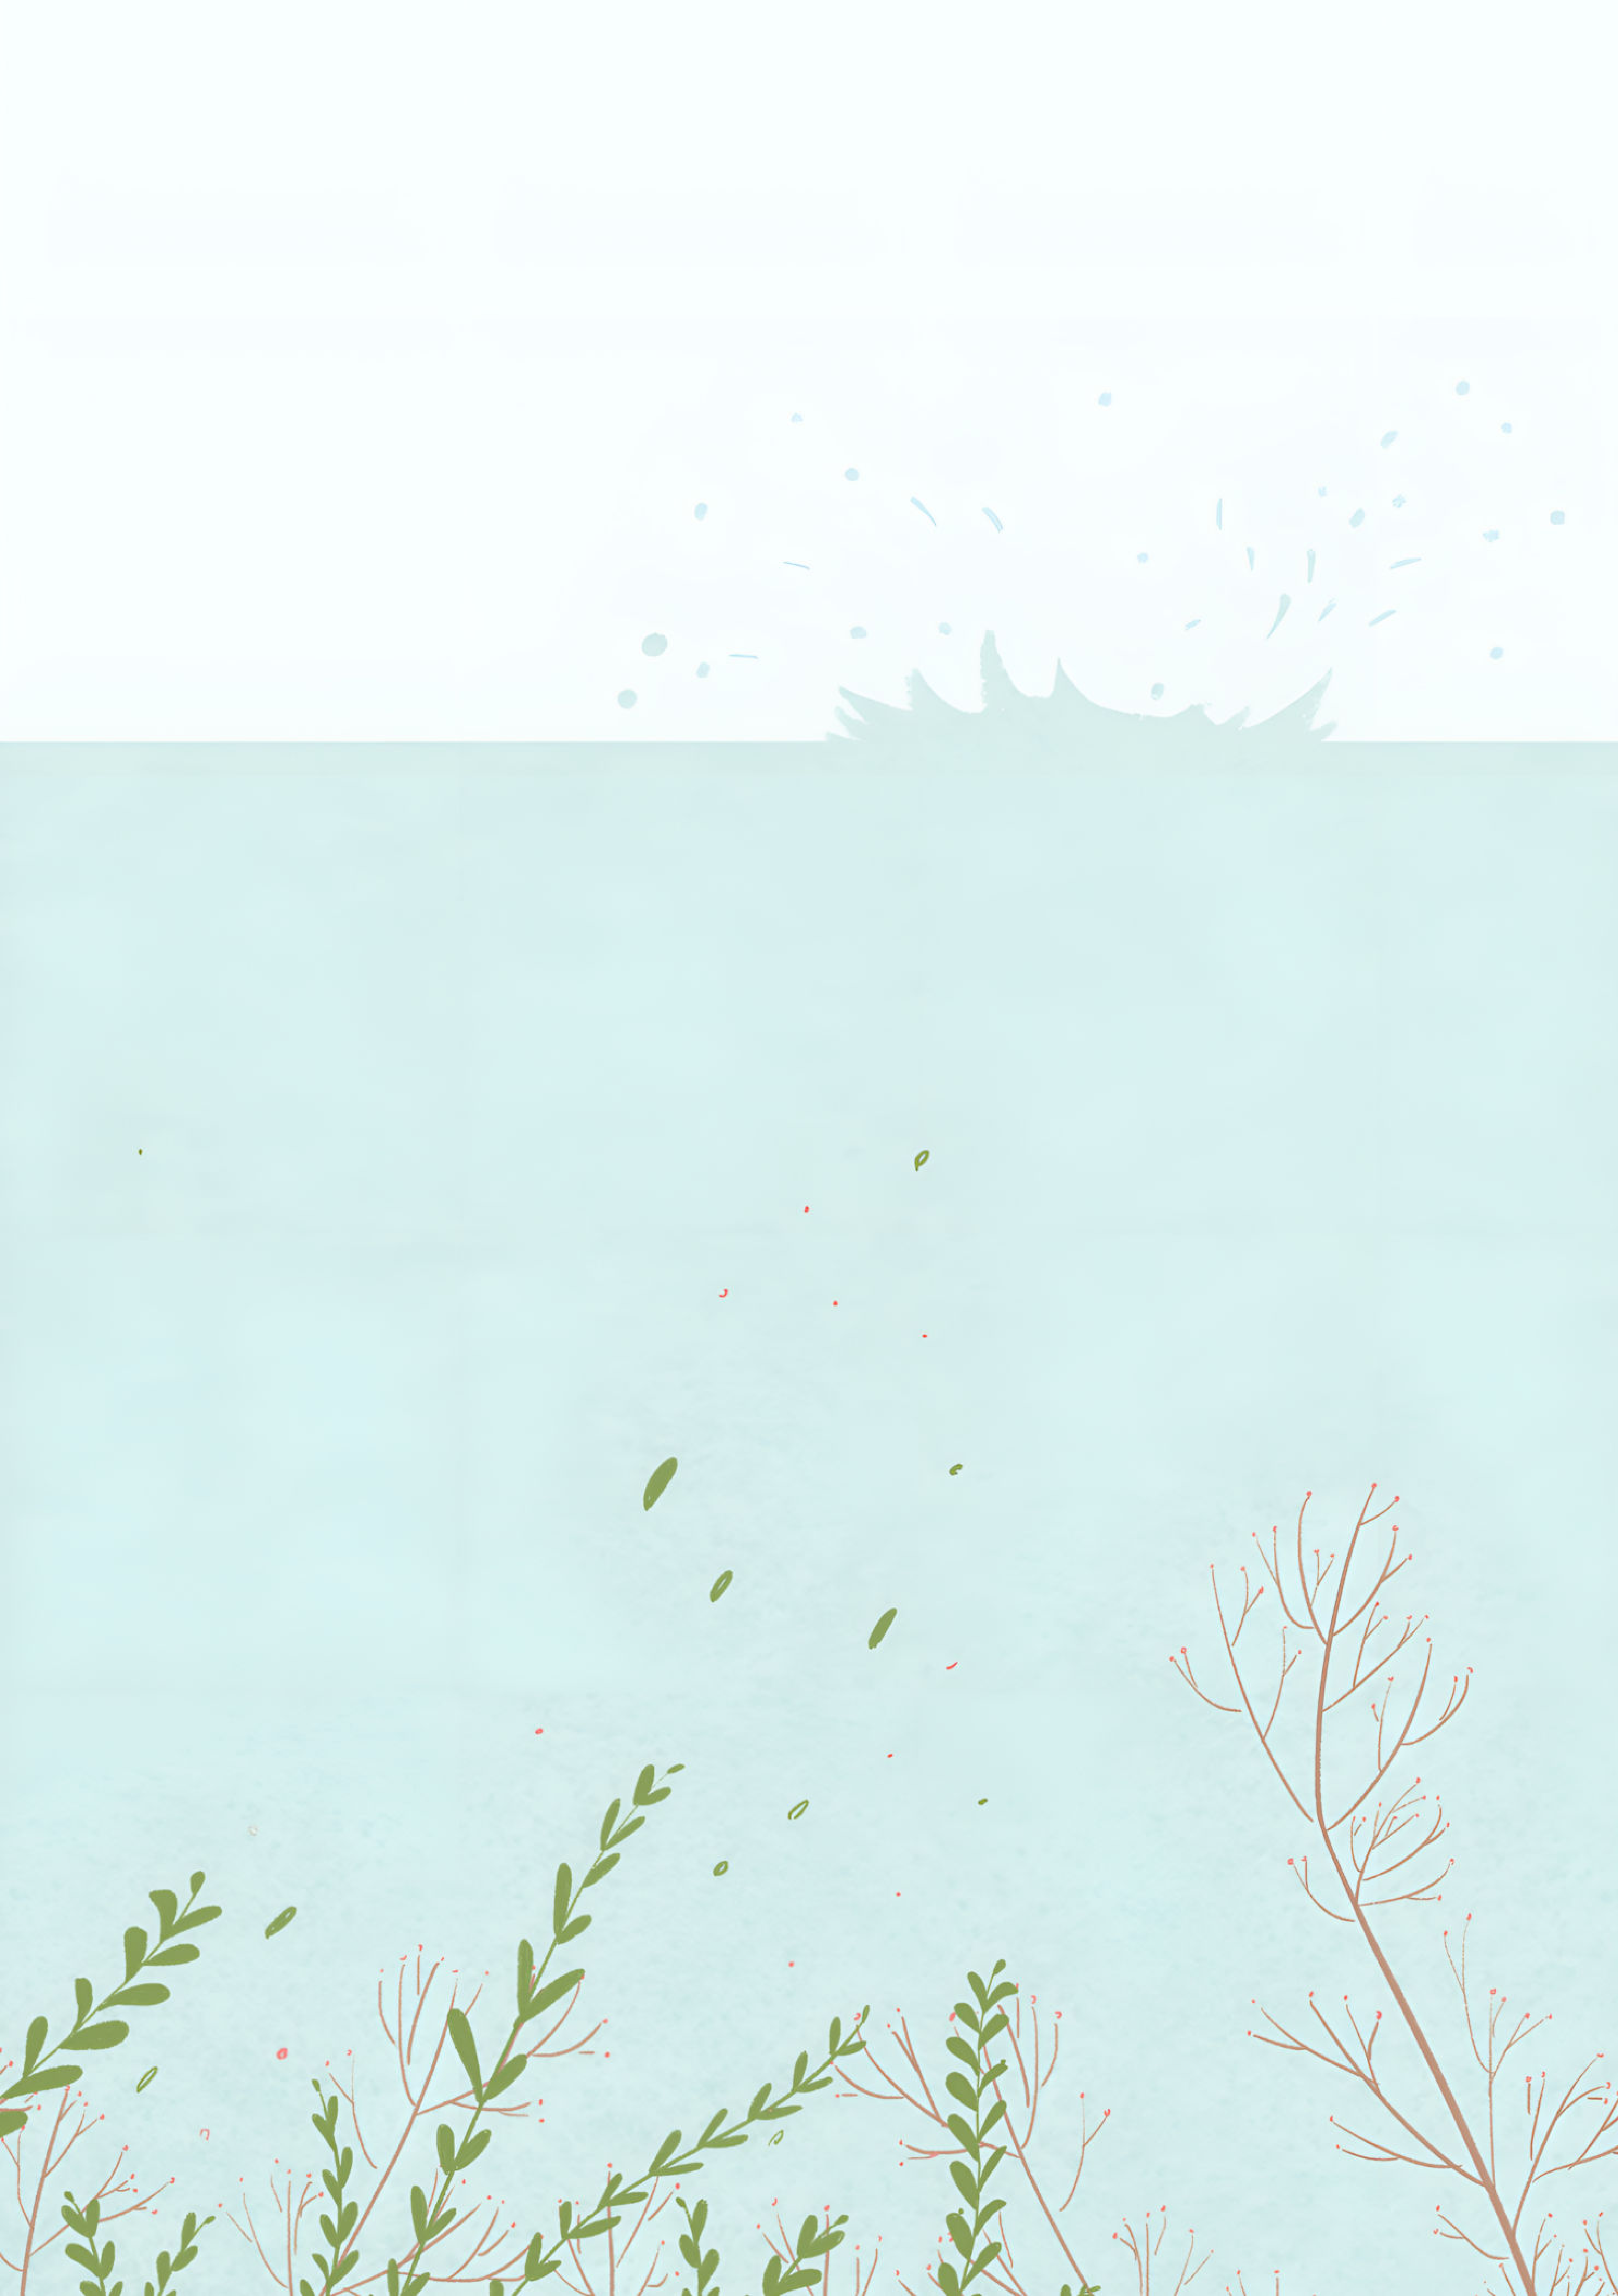
\includepdf{back.pdf}
\end{document}
